For each dataset we independently compared clustering scores of different algorithms for multiple distances. For the algorithms that require a predefined number of clusters we set the value k to be the number of different classes in the dataset (except for the diabetes dataset, which does not have categorical labels). \\

\begin{figure}[H]
	\centering
	\subfloat[ARI ]{{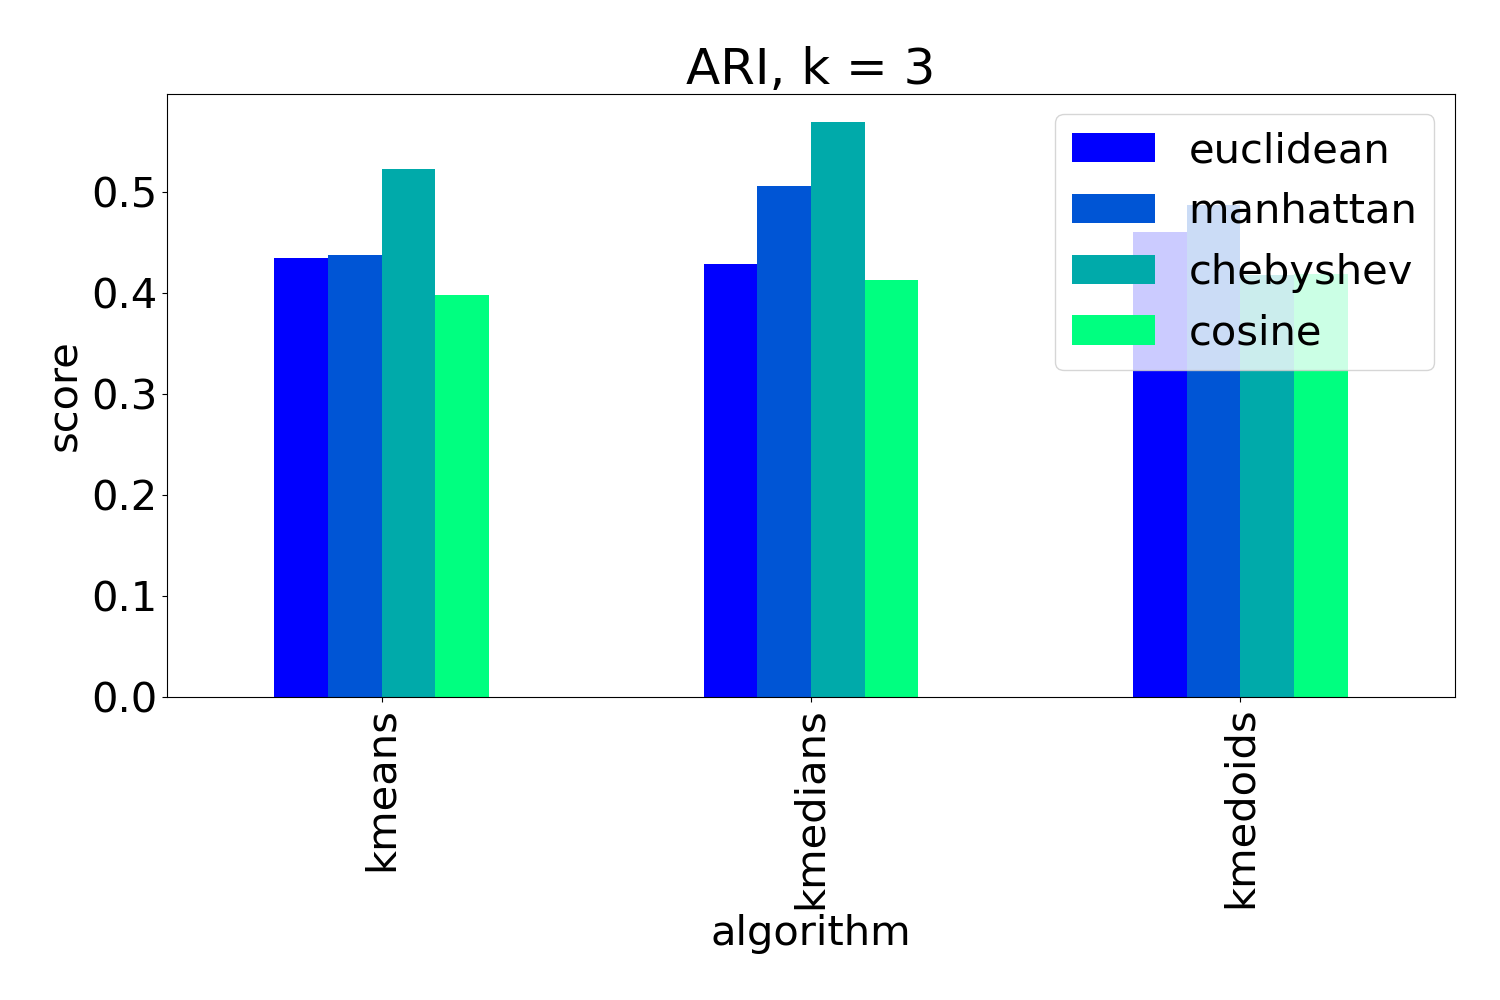
\includegraphics[width=0.45\textwidth]{../plots/iris/combined/ARI/algdist_for_given_k.png} }}%
	\qquad
	\subfloat[NMI ]{{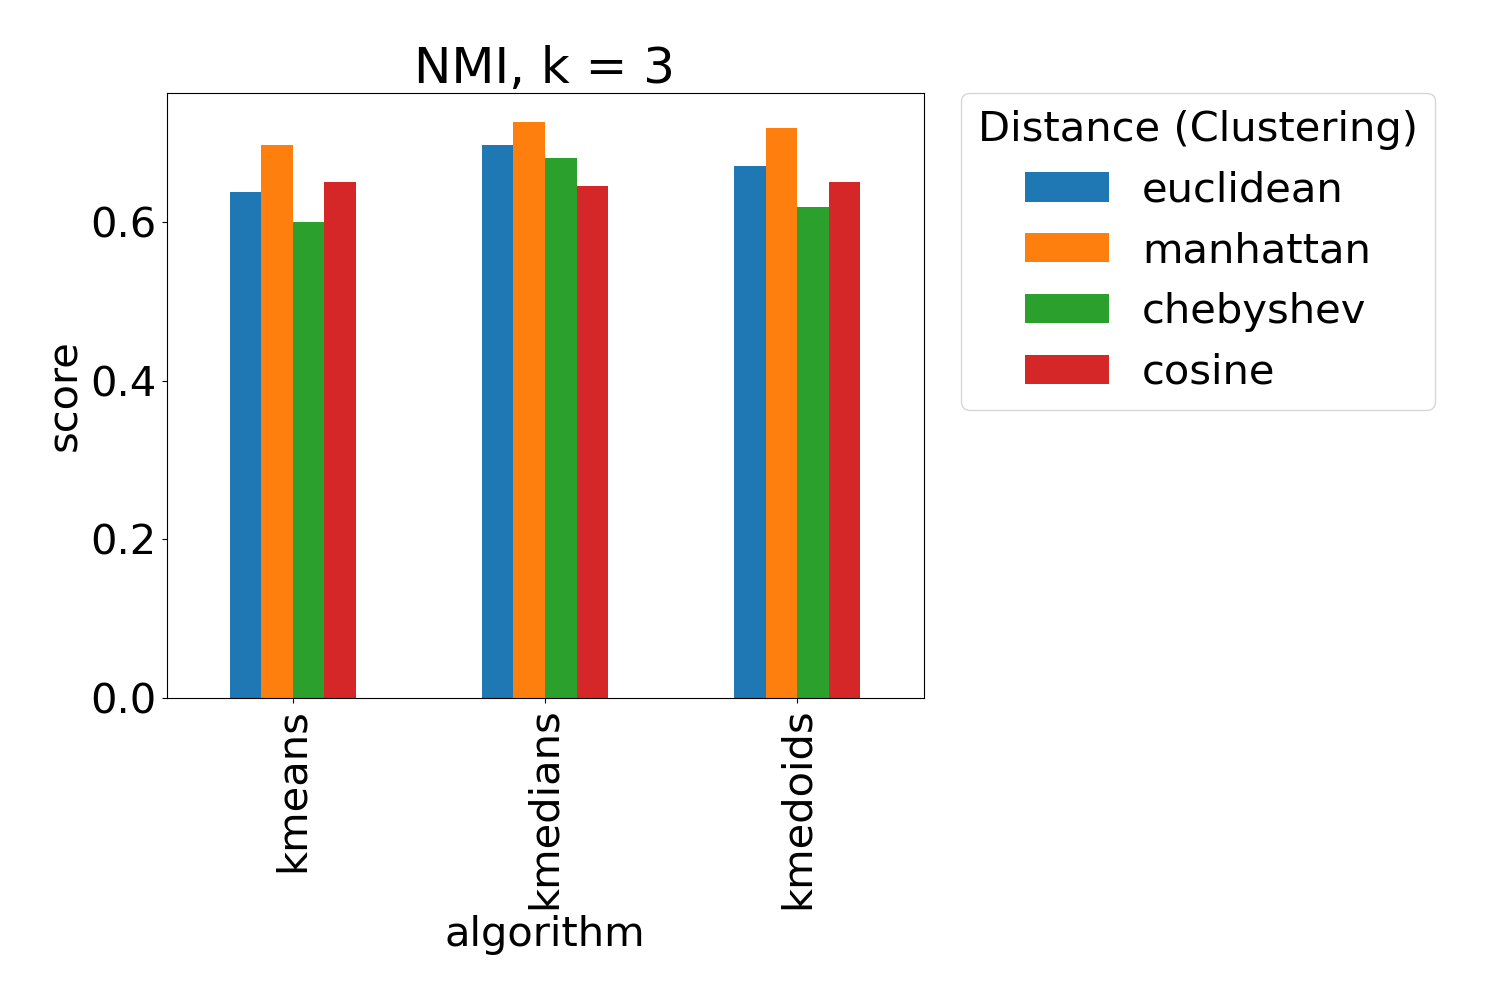
\includegraphics[width=0.45\textwidth]{../plots/iris/combined/NMI/algdist_for_given_k.png} }}%
	\qquad
	\subfloat[Completeness Score ]{{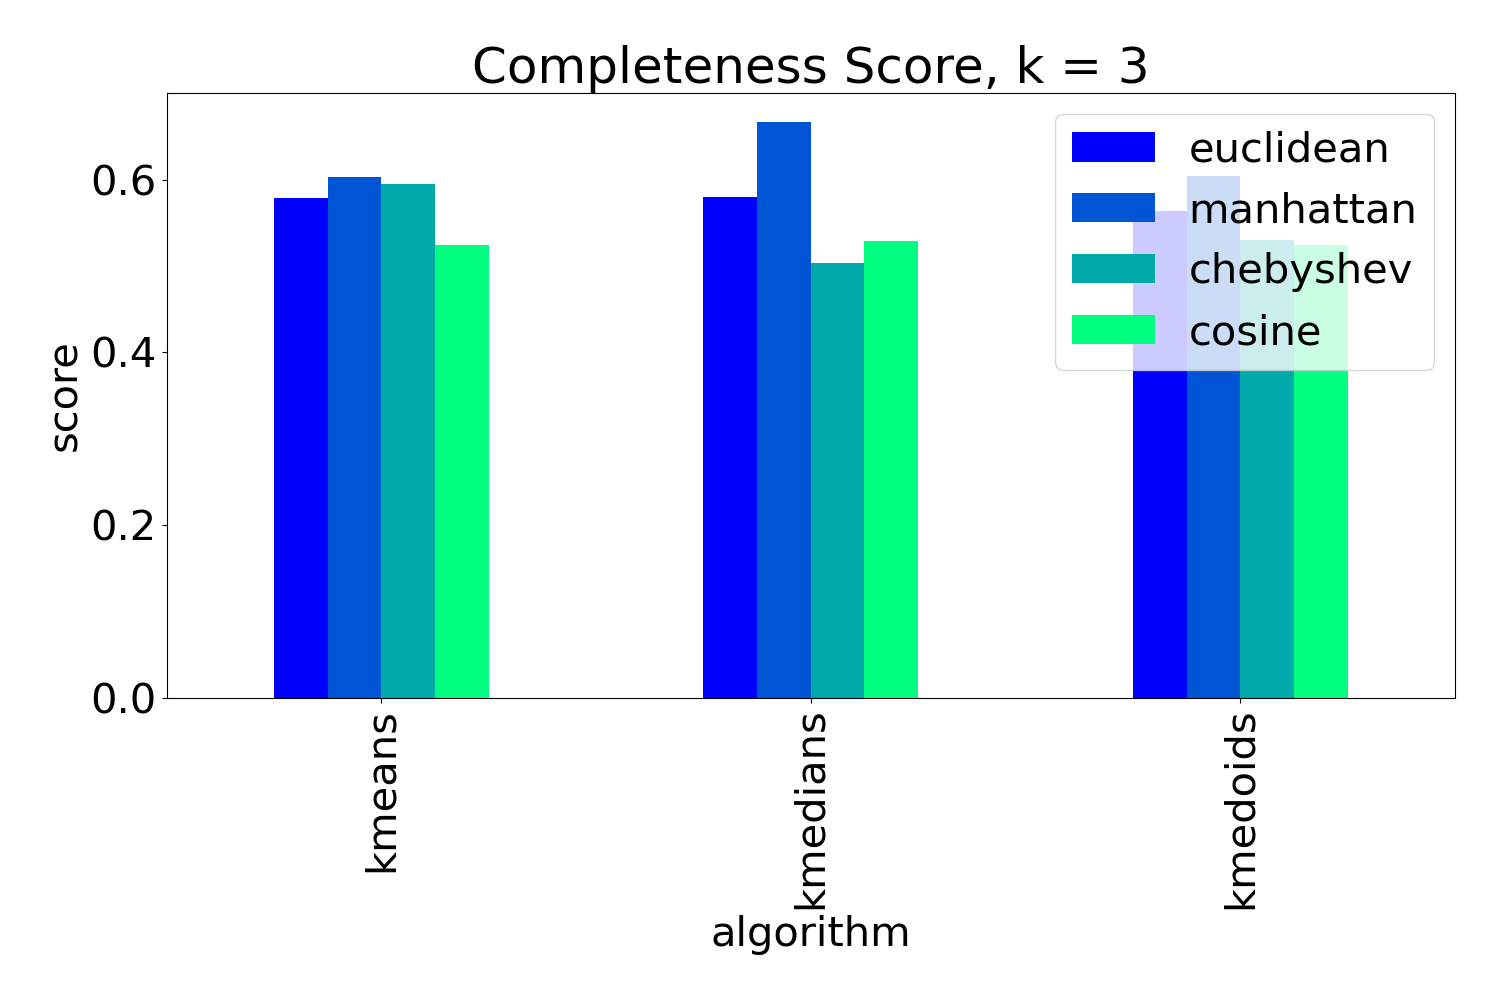
\includegraphics[width=0.45\textwidth]{../plots/iris/combined/Completeness Score/algdist_for_given_k.png} }}%
	\qquad
	\subfloat[Homogeneity Score ]{{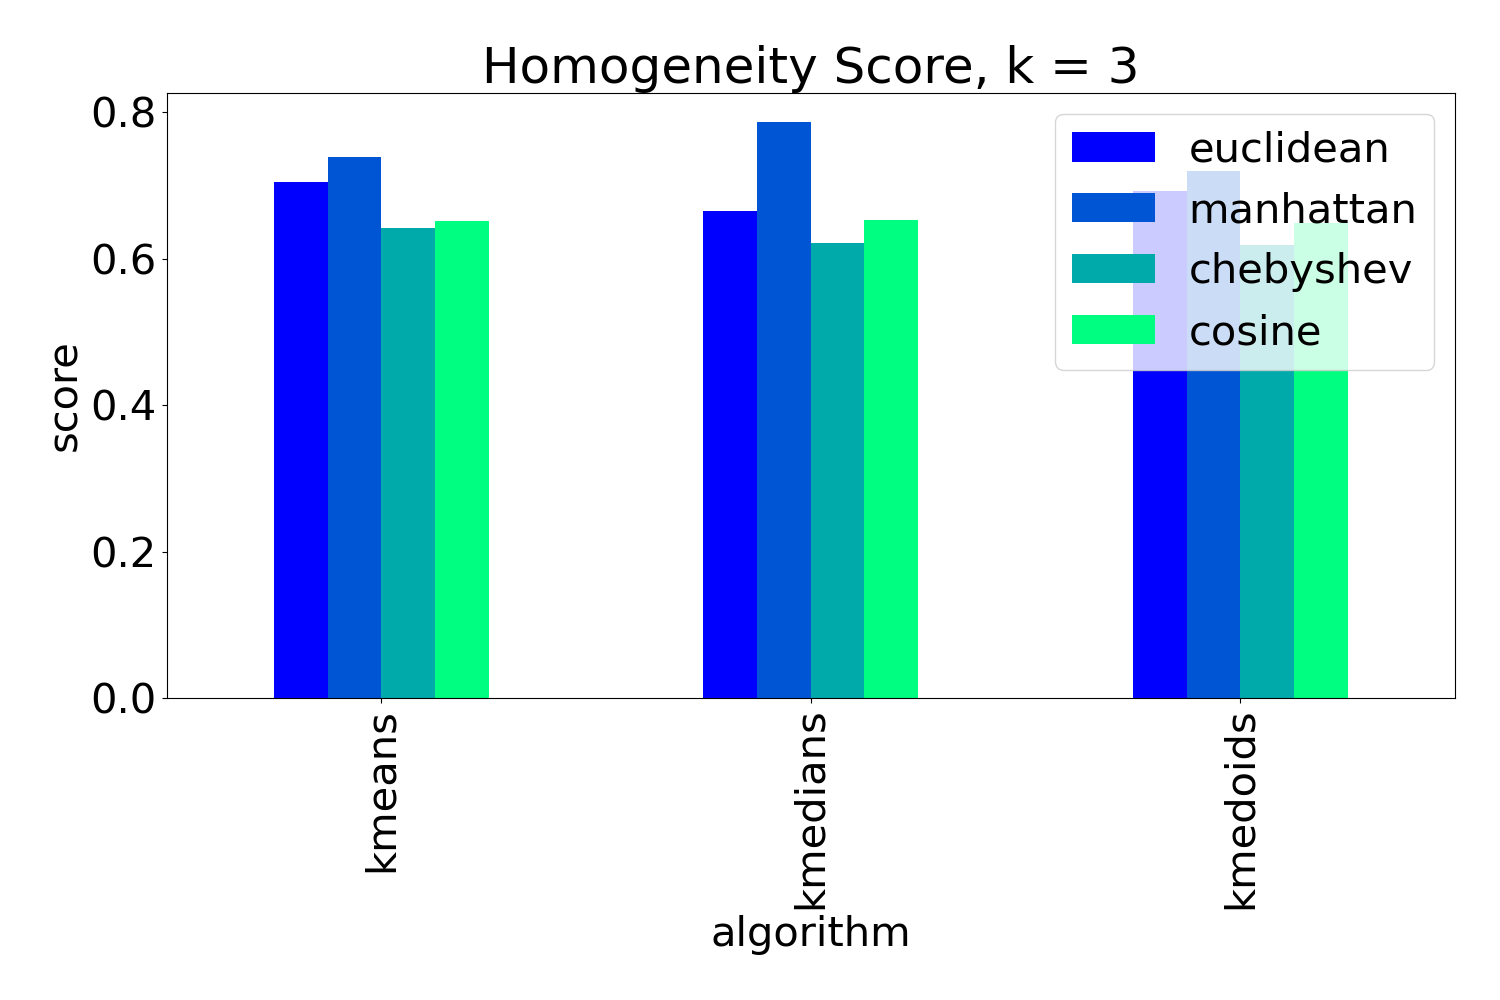
\includegraphics[width=0.45\textwidth]{../plots/iris/combined/Homogeneity Score/algdist_for_given_k.png} }}%
	\qquad
	\subfloat[Silhouette Score ]{{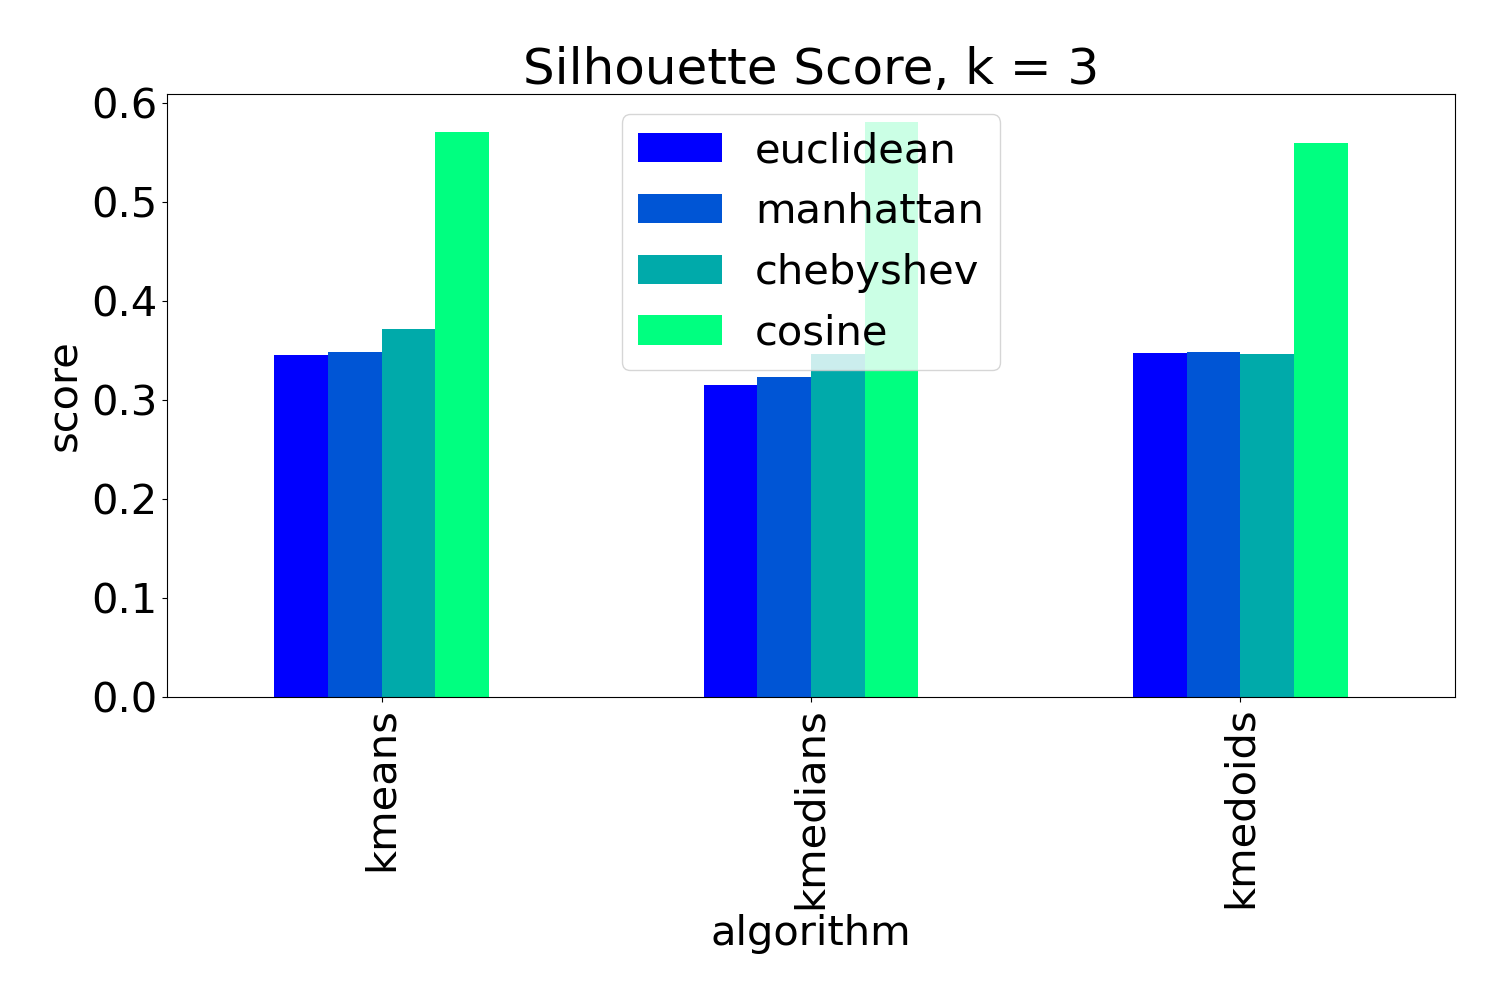
\includegraphics[width=0.45\textwidth]{../plots/iris/combined/Silhouette Score/algdist_for_given_k.png} }}%
	
	\caption{Comparison of clustering scores for Iris dataset (given k=3)}%
\end{figure}

\begin{figure}[H]
	\centering
	\subfloat[ARI ]{{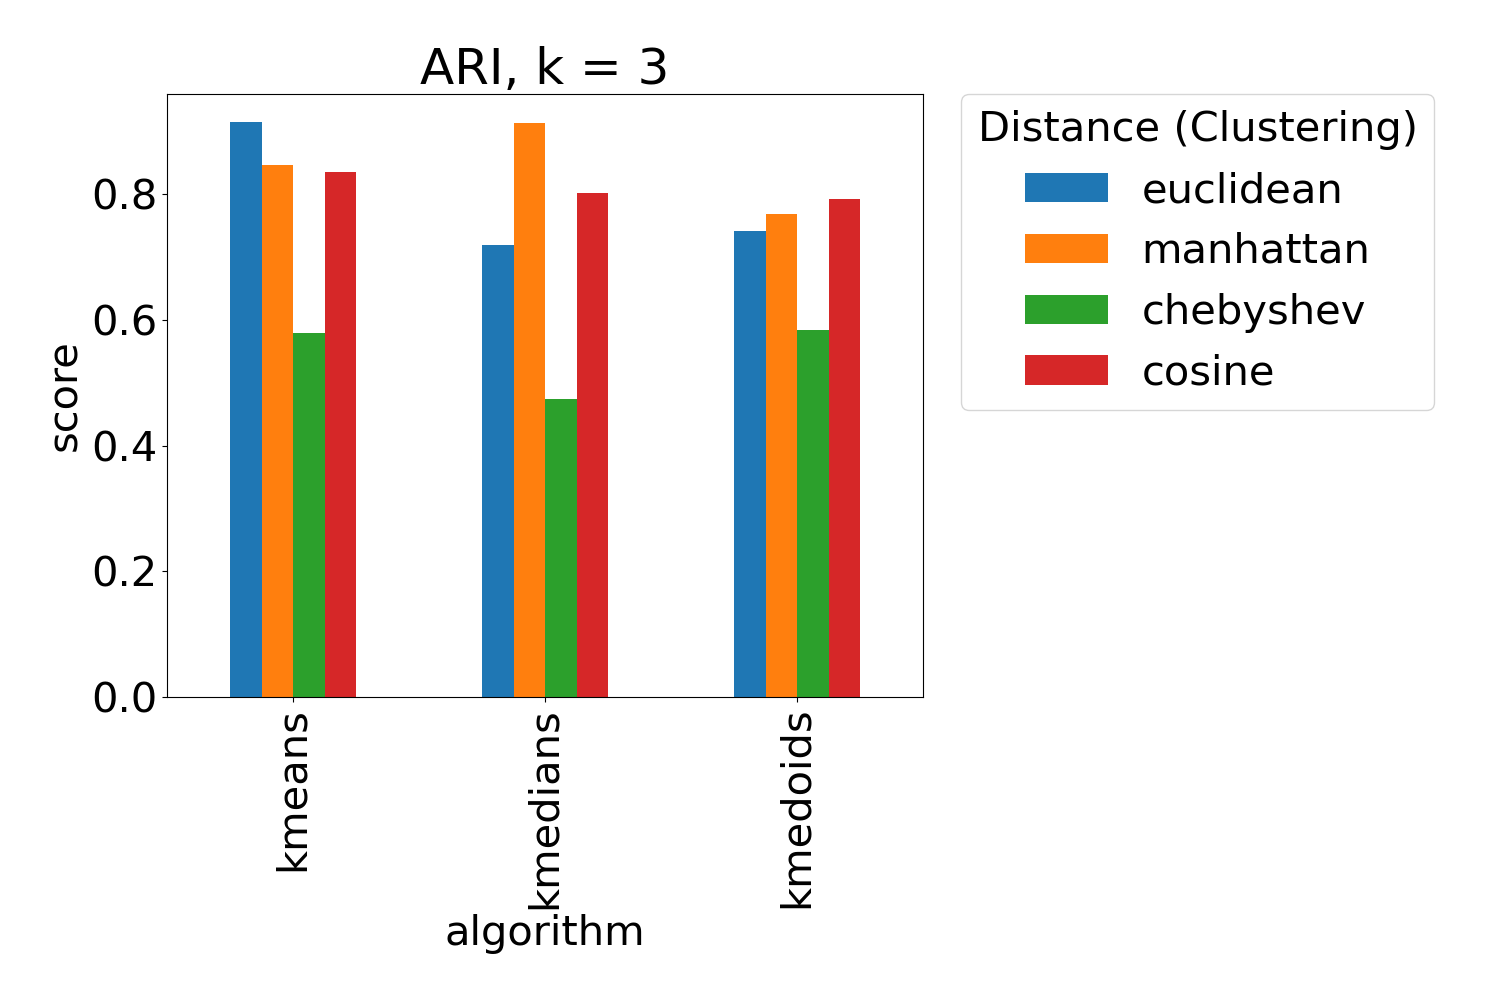
\includegraphics[width=0.45\textwidth]{../plots/wine/combined/ARI/algdist_for_given_k.png} }}%
	\qquad
	\subfloat[NMI ]{{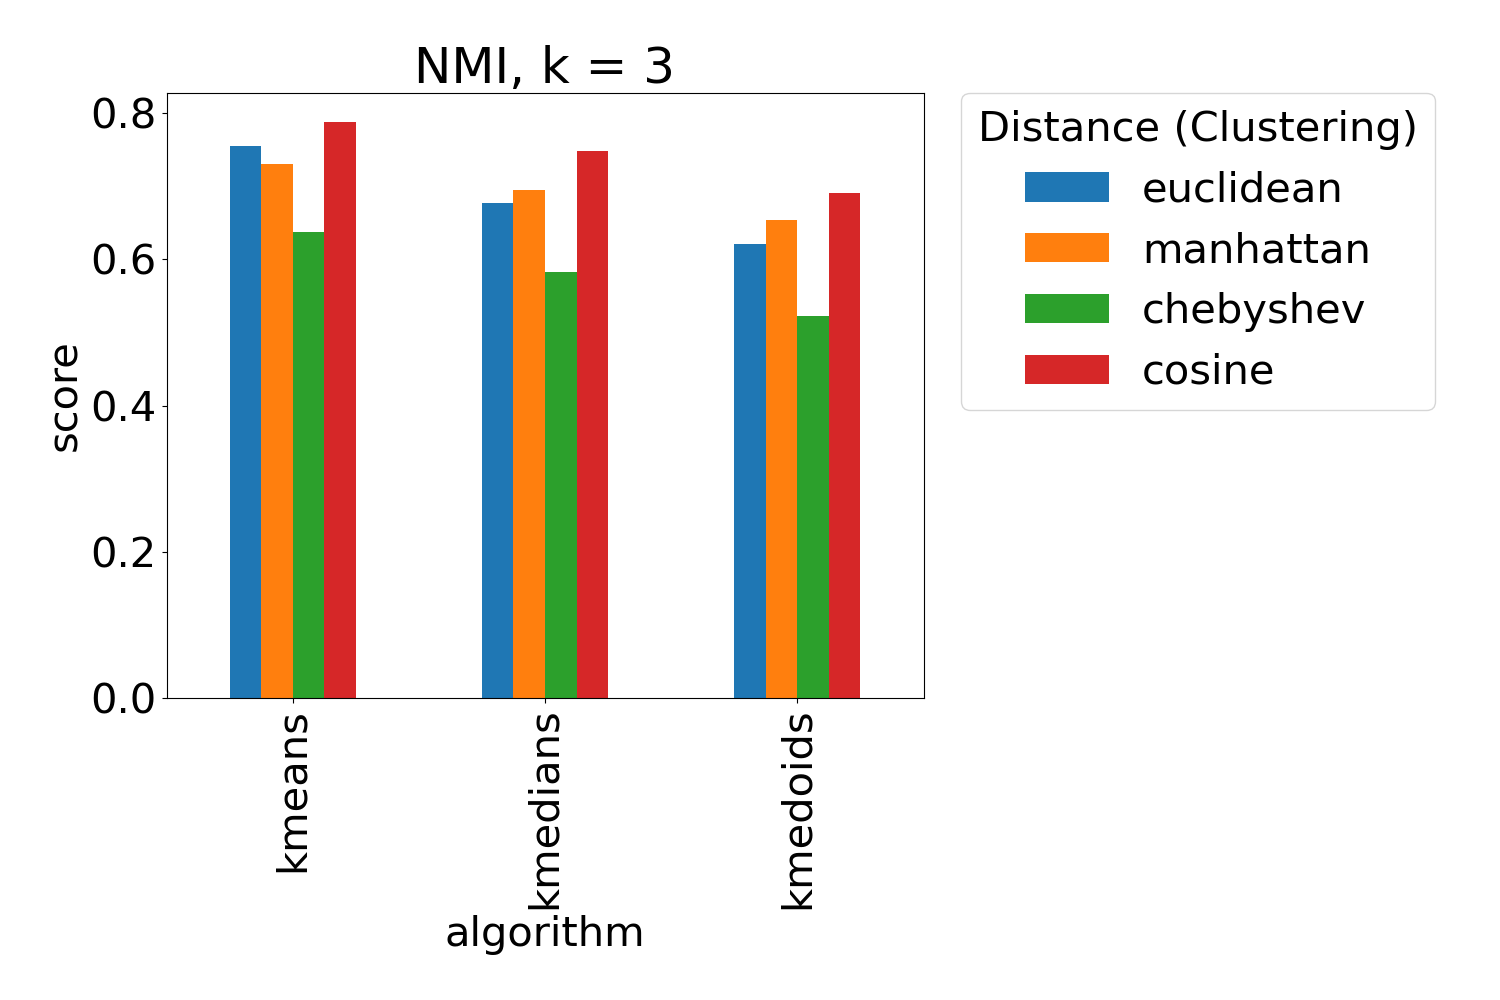
\includegraphics[width=0.45\textwidth]{../plots/wine/combined/NMI/algdist_for_given_k.png} }}%
	\qquad
	\subfloat[Completeness Score ]{{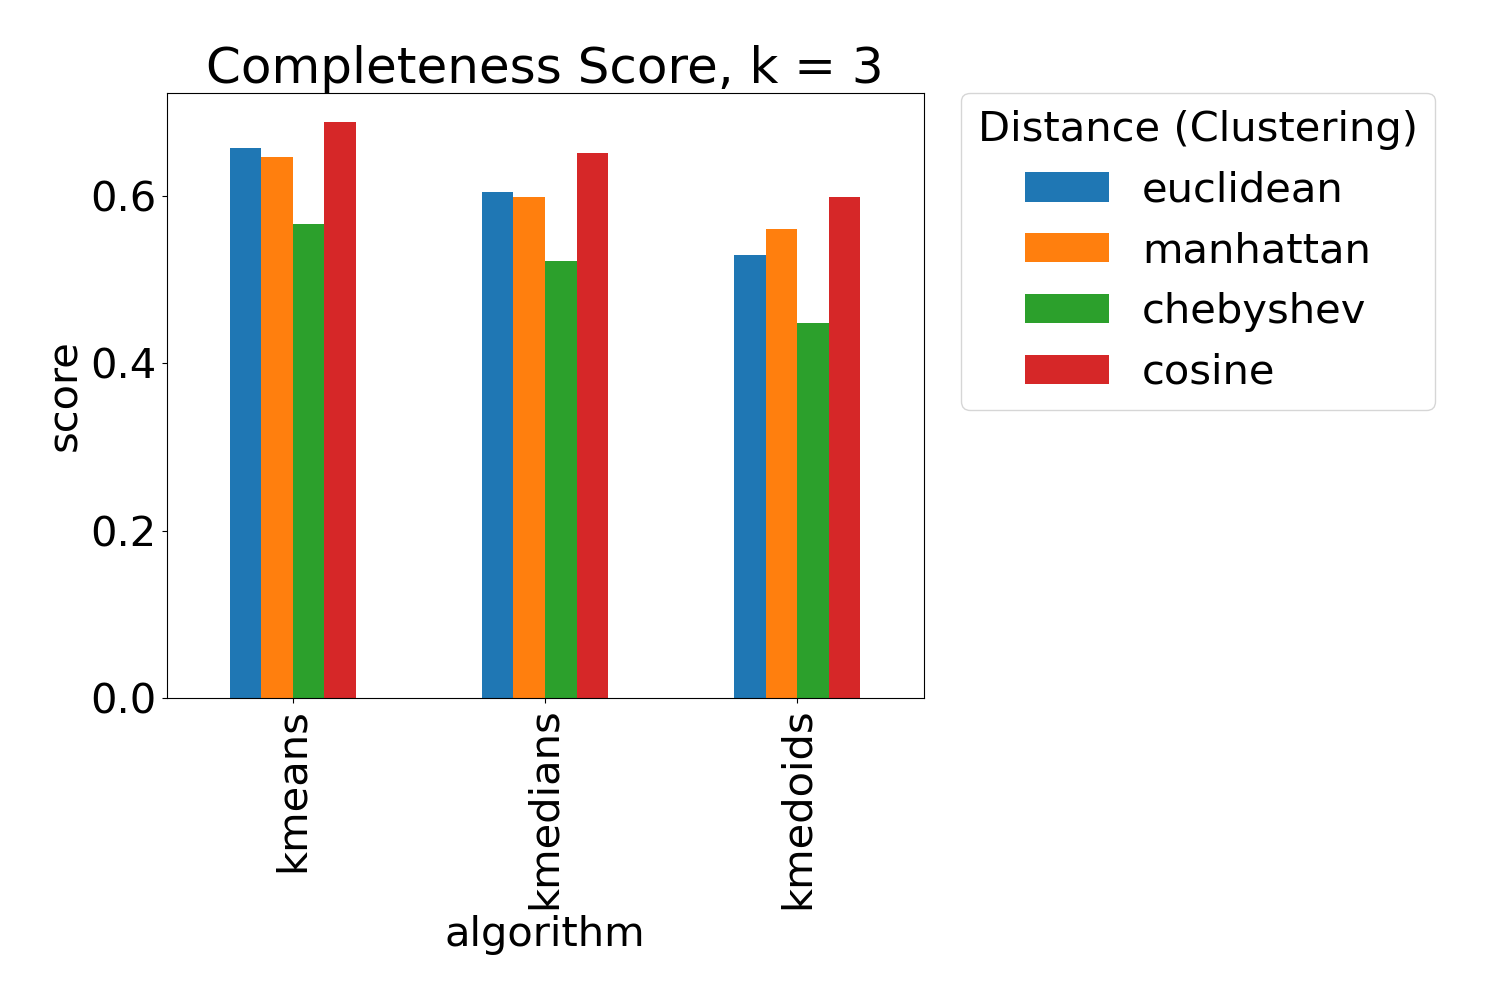
\includegraphics[width=0.45\textwidth]{../plots/wine/combined/Completeness Score/algdist_for_given_k.png} }}%
	\qquad
	\subfloat[Homogeneity Score ]{{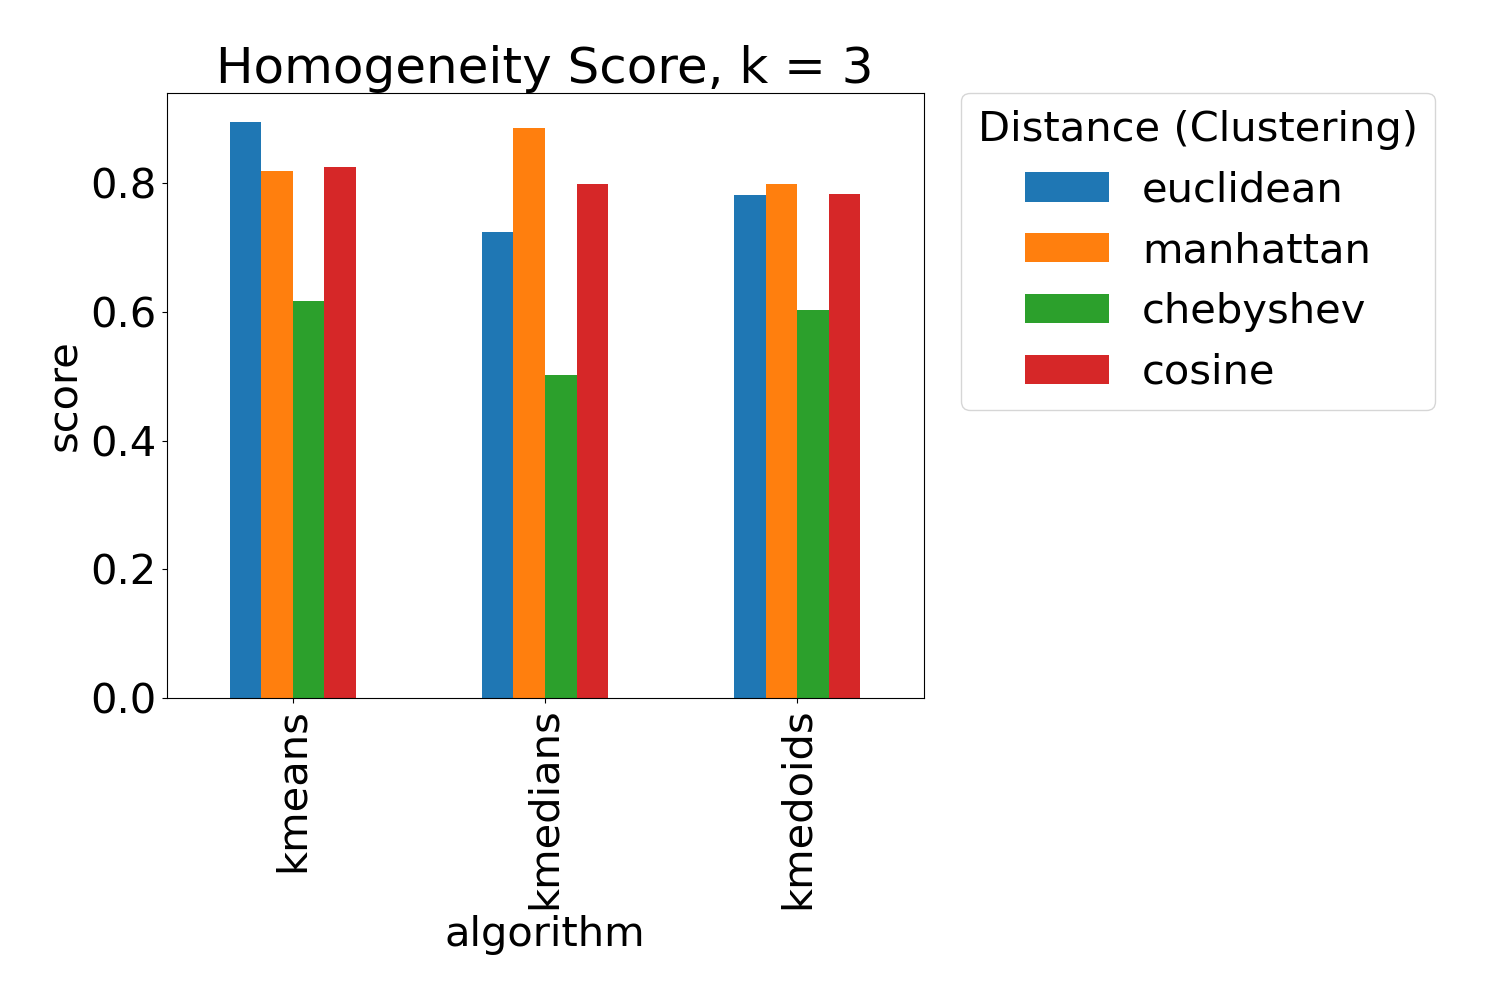
\includegraphics[width=0.45\textwidth]{../plots/wine/combined/Homogeneity Score/algdist_for_given_k.png} }}%
	\qquad
	\subfloat[Silhouette Score ]{{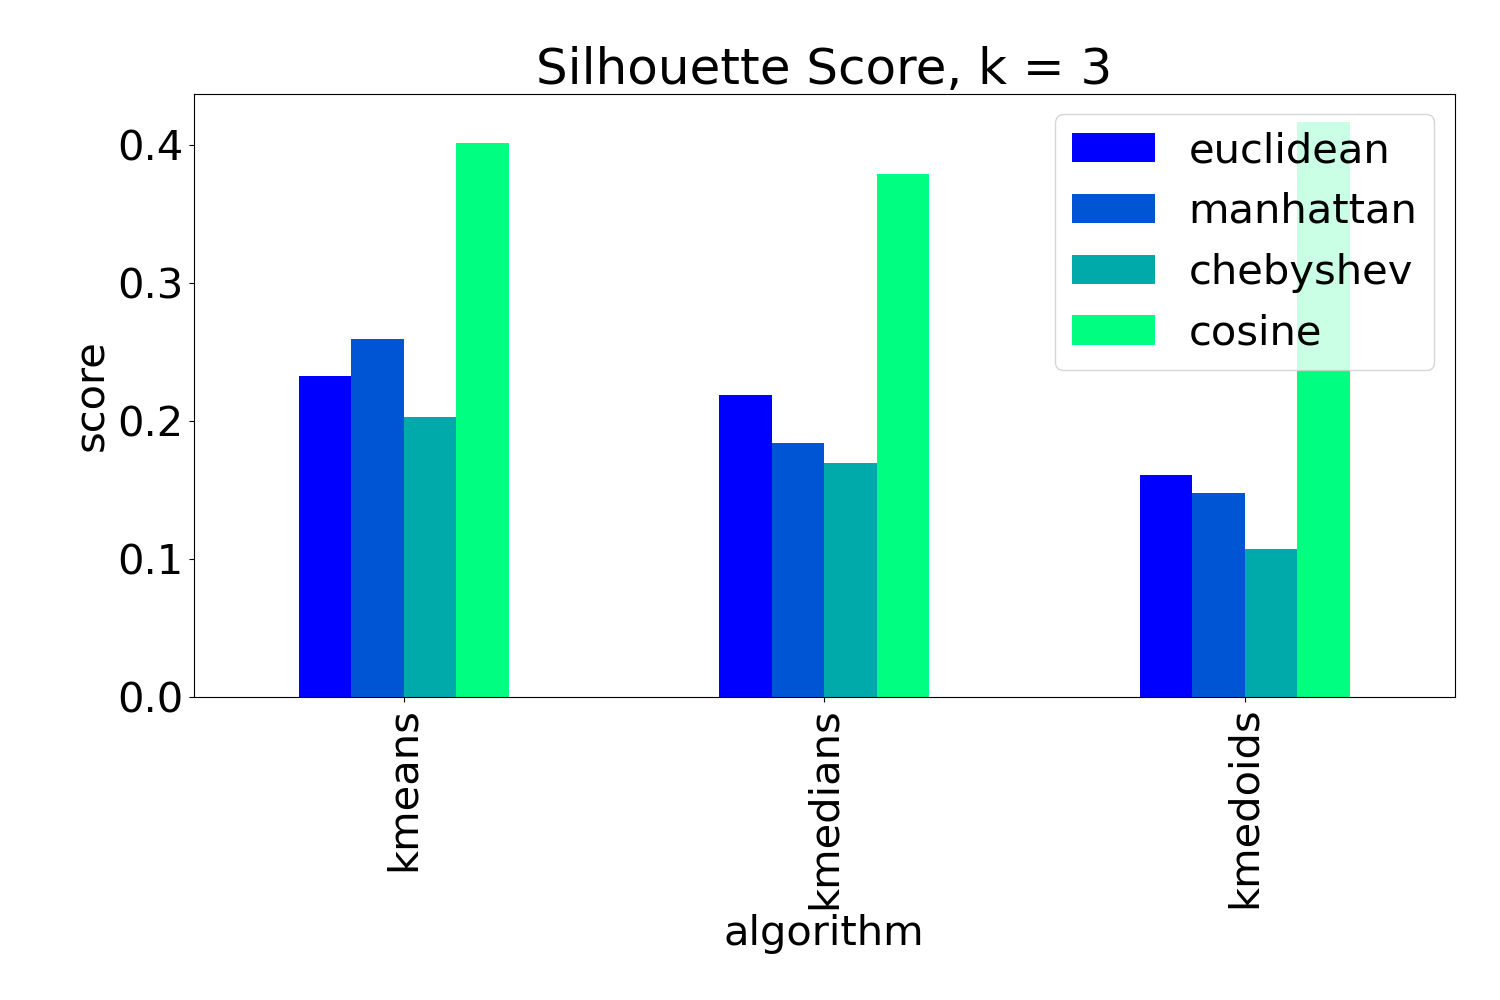
\includegraphics[width=0.45\textwidth]{../plots/wine/combined/Silhouette Score/algdist_for_given_k.png} }}%
	
	\caption{Comparison of clustering scores for Wine dataset (given k=3)}%
\end{figure}

\begin{figure}[H]
	\centering
	\subfloat[ARI ]{{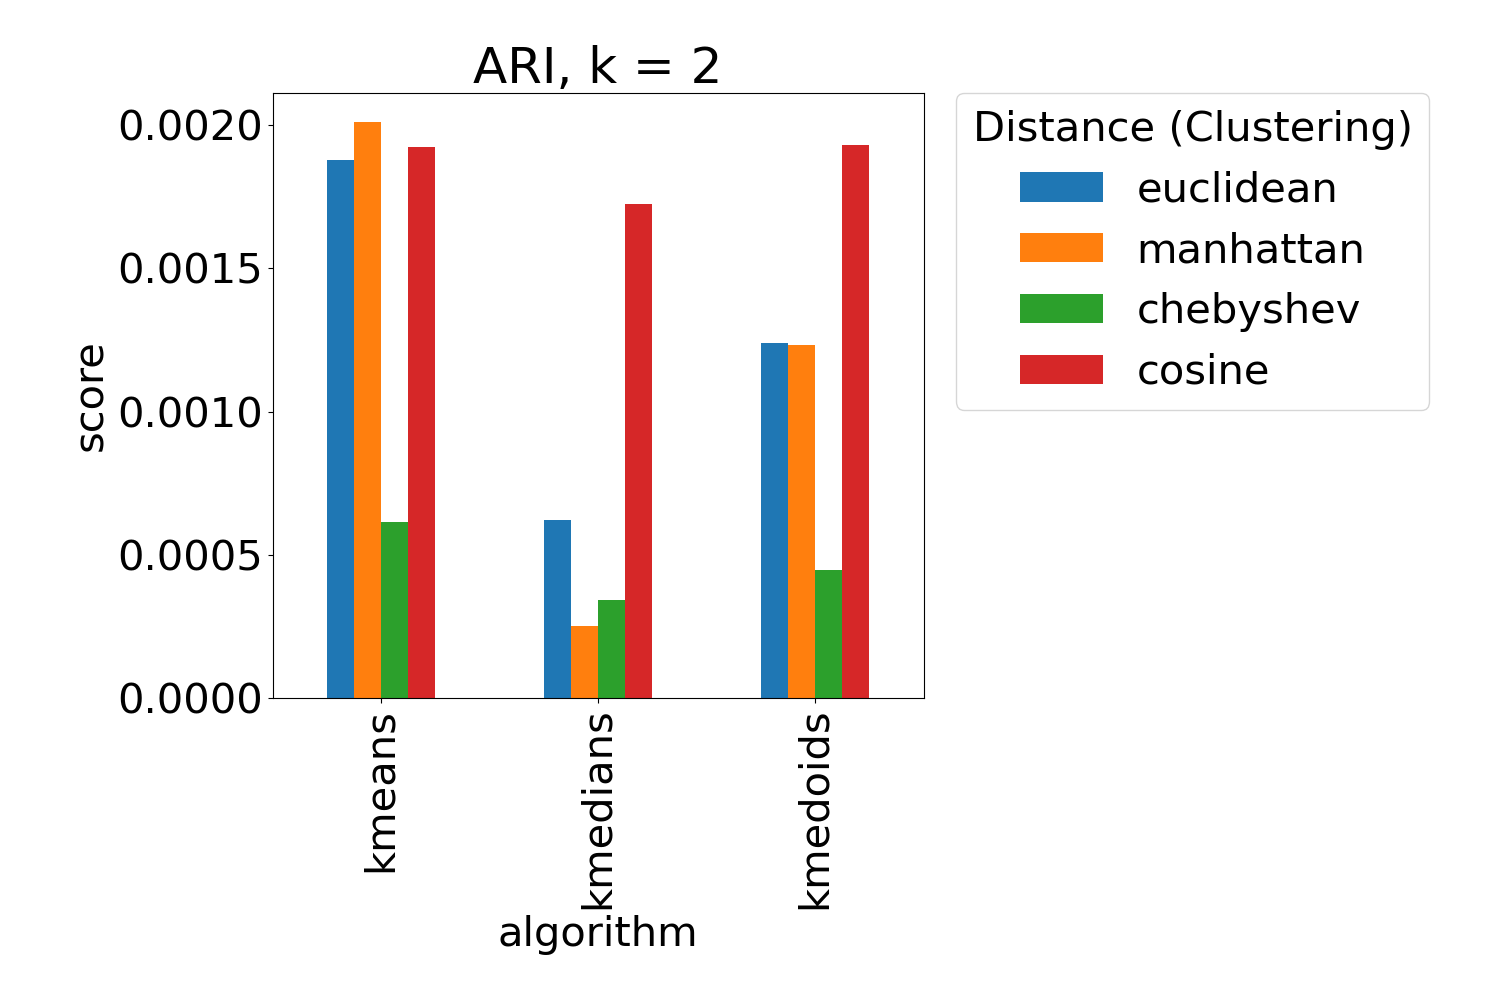
\includegraphics[width=0.45\textwidth]{../plots/diabetes/combined/ARI/algdist_for_given_k.png} }}%
	\qquad
	\subfloat[NMI ]{{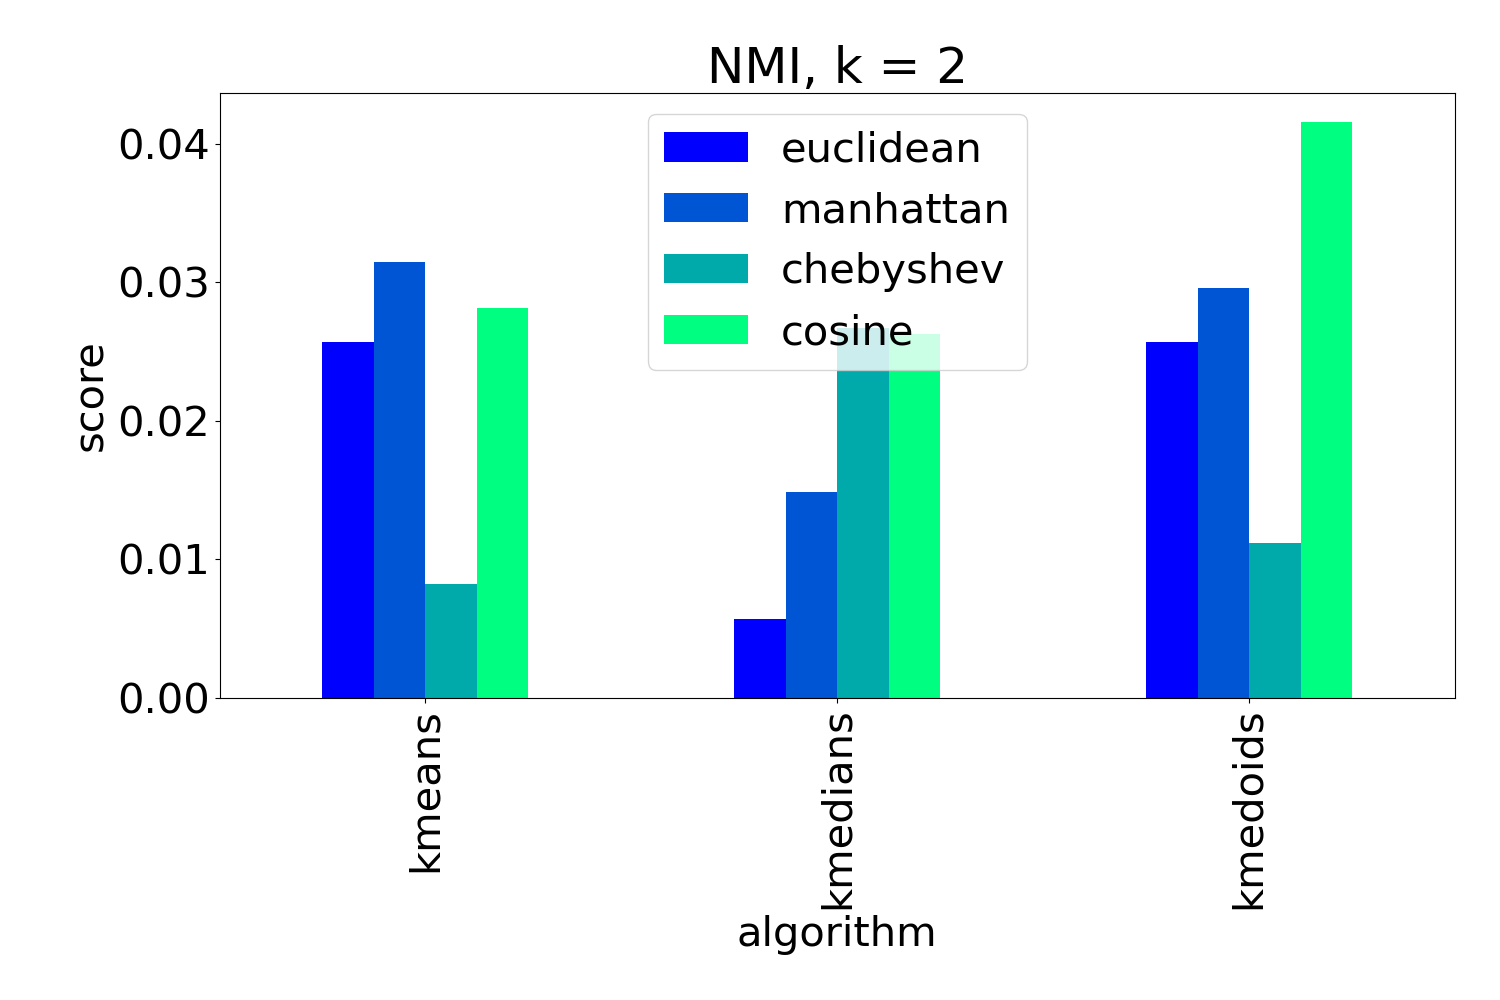
\includegraphics[width=0.45\textwidth]{../plots/diabetes/combined/NMI/algdist_for_given_k.png} }}%
	\qquad
	\subfloat[Completeness Score ]{{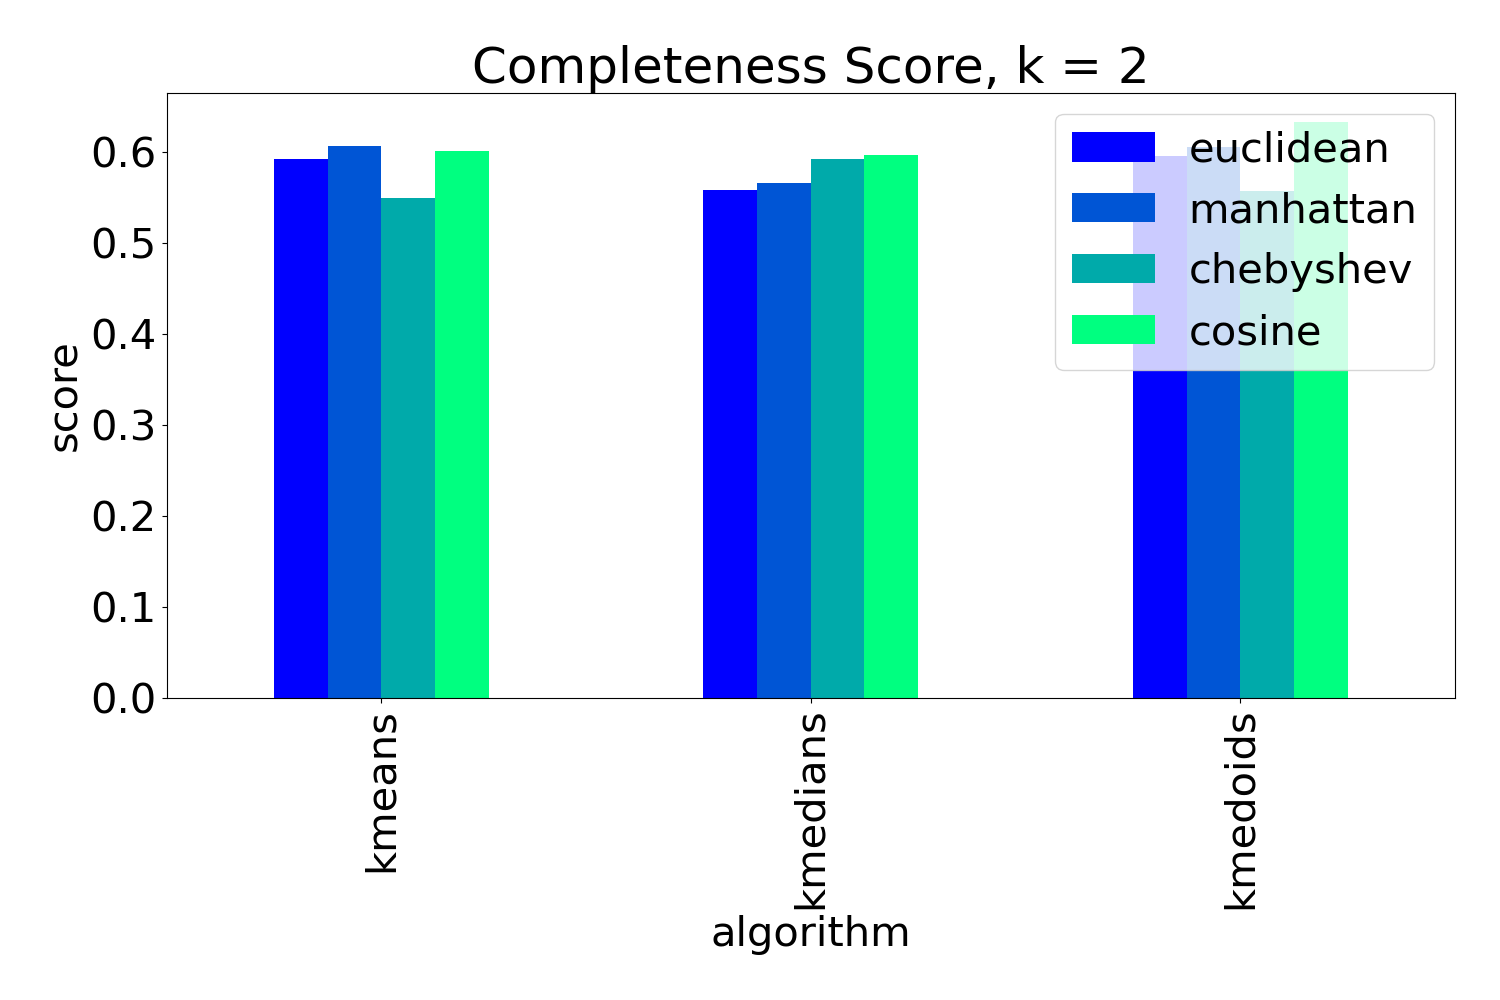
\includegraphics[width=0.45\textwidth]{../plots/diabetes/combined/Completeness Score/algdist_for_given_k.png} }}%
	\qquad
	\subfloat[Homogeneity Score ]{{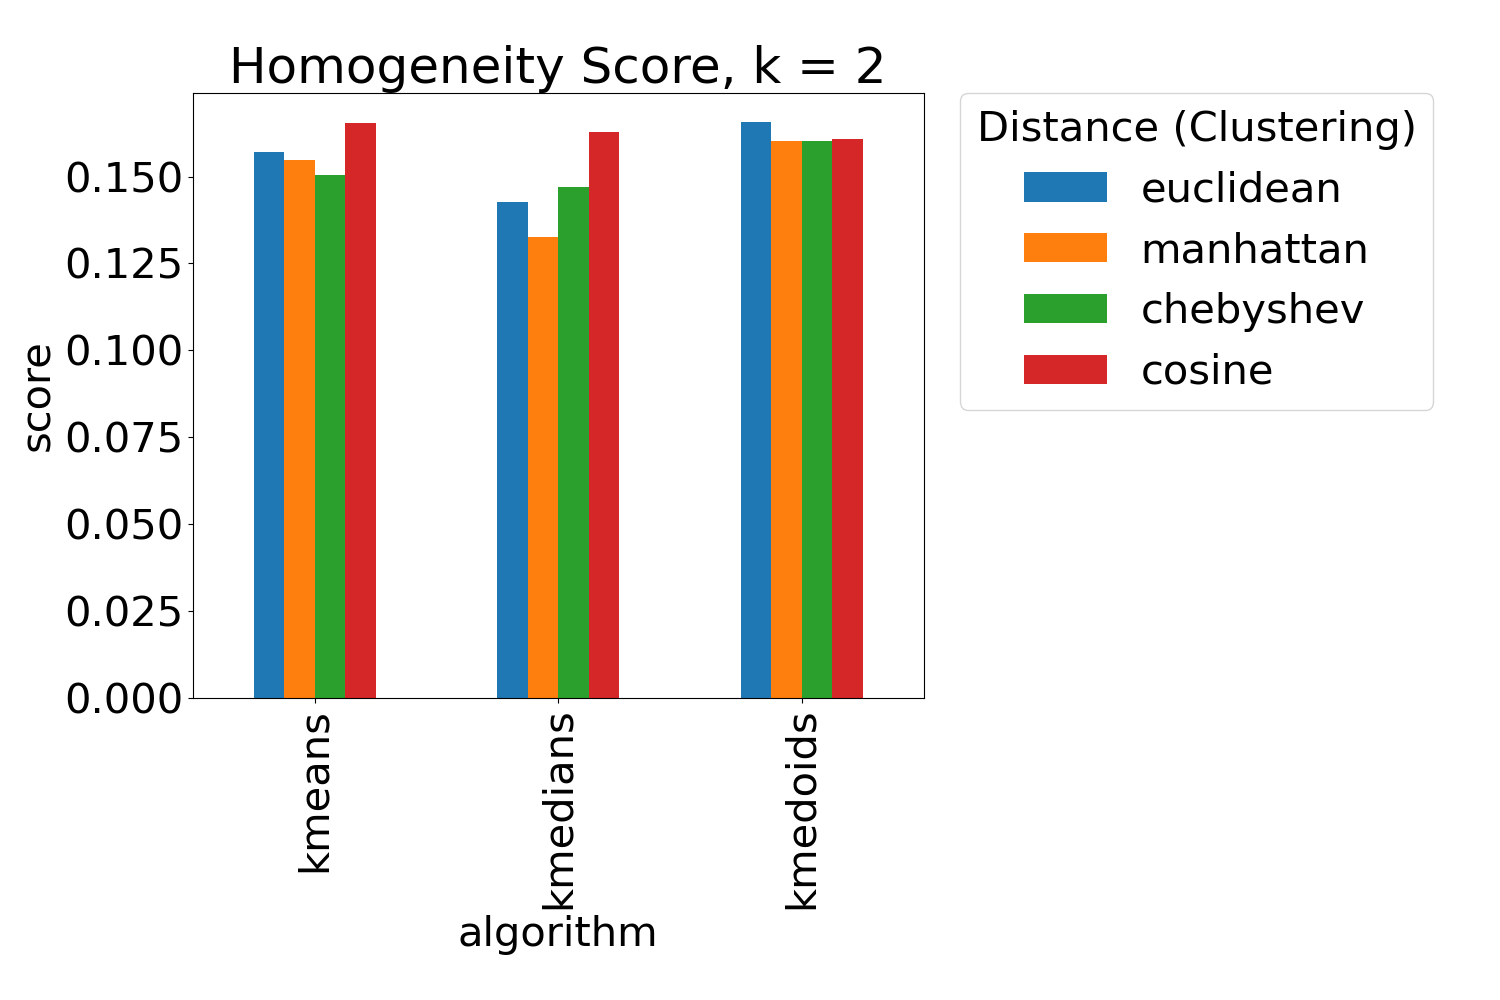
\includegraphics[width=0.45\textwidth]{../plots/diabetes/combined/Homogeneity Score/algdist_for_given_k.png} }}%
	\qquad
	\subfloat[Silhouette Score ]{{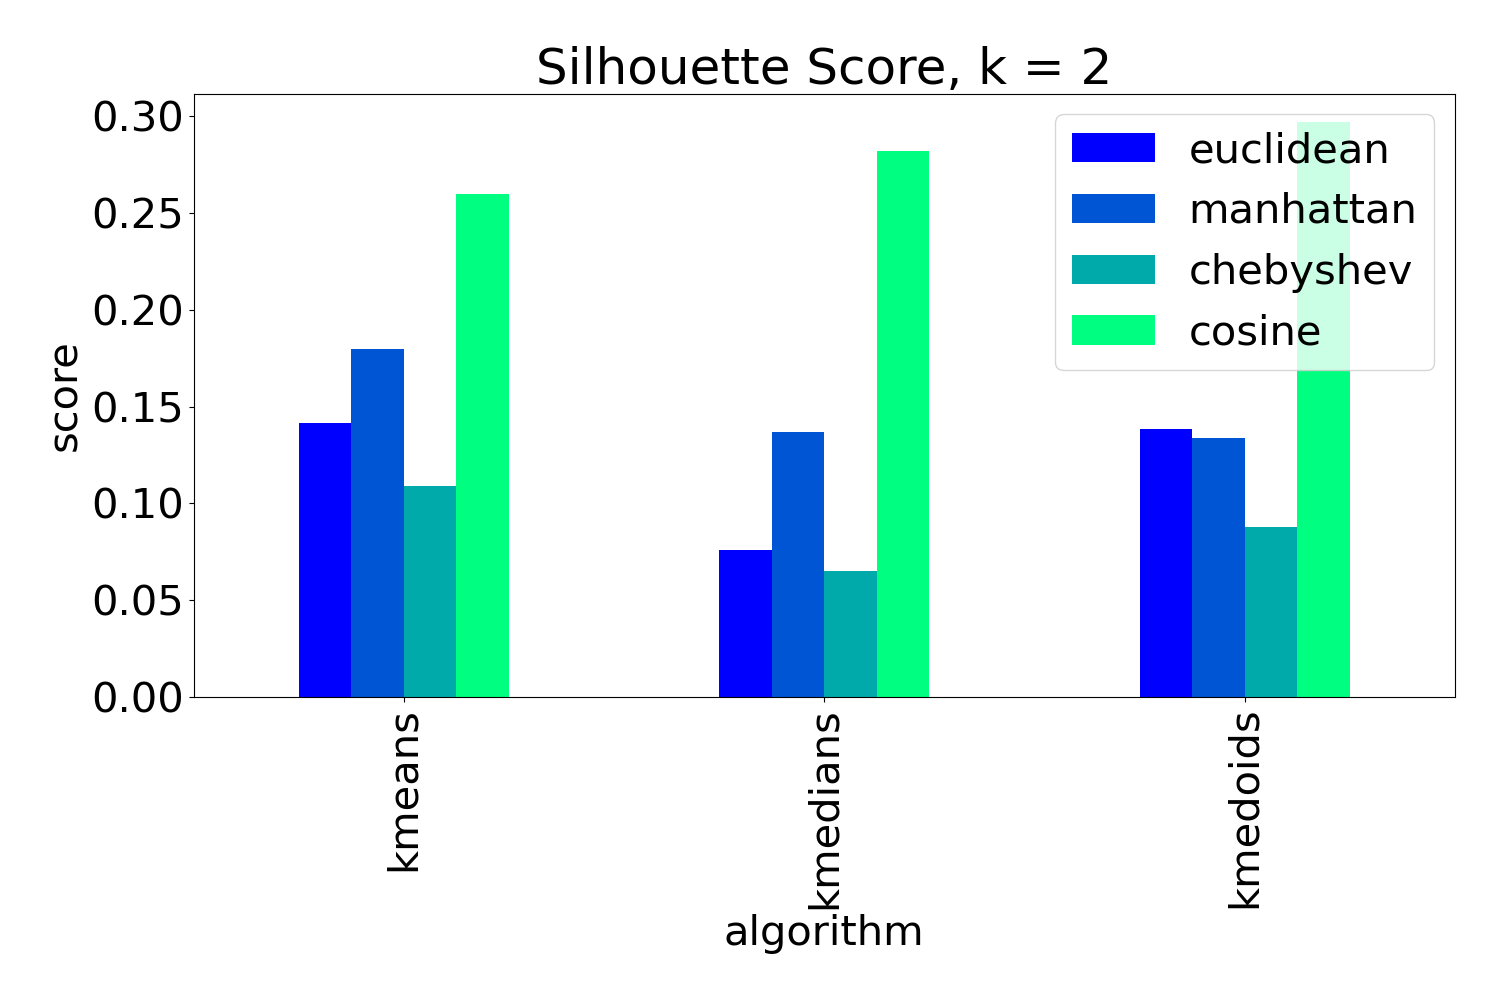
\includegraphics[width=0.45\textwidth]{../plots/diabetes/combined/Silhouette Score/algdist_for_given_k.png} }}%
	
	\caption{Comparison of clustering scores for Diabetes dataset (given k=2)}%
\end{figure}

\begin{figure}[H]
	\centering
	\subfloat[ARI ]{{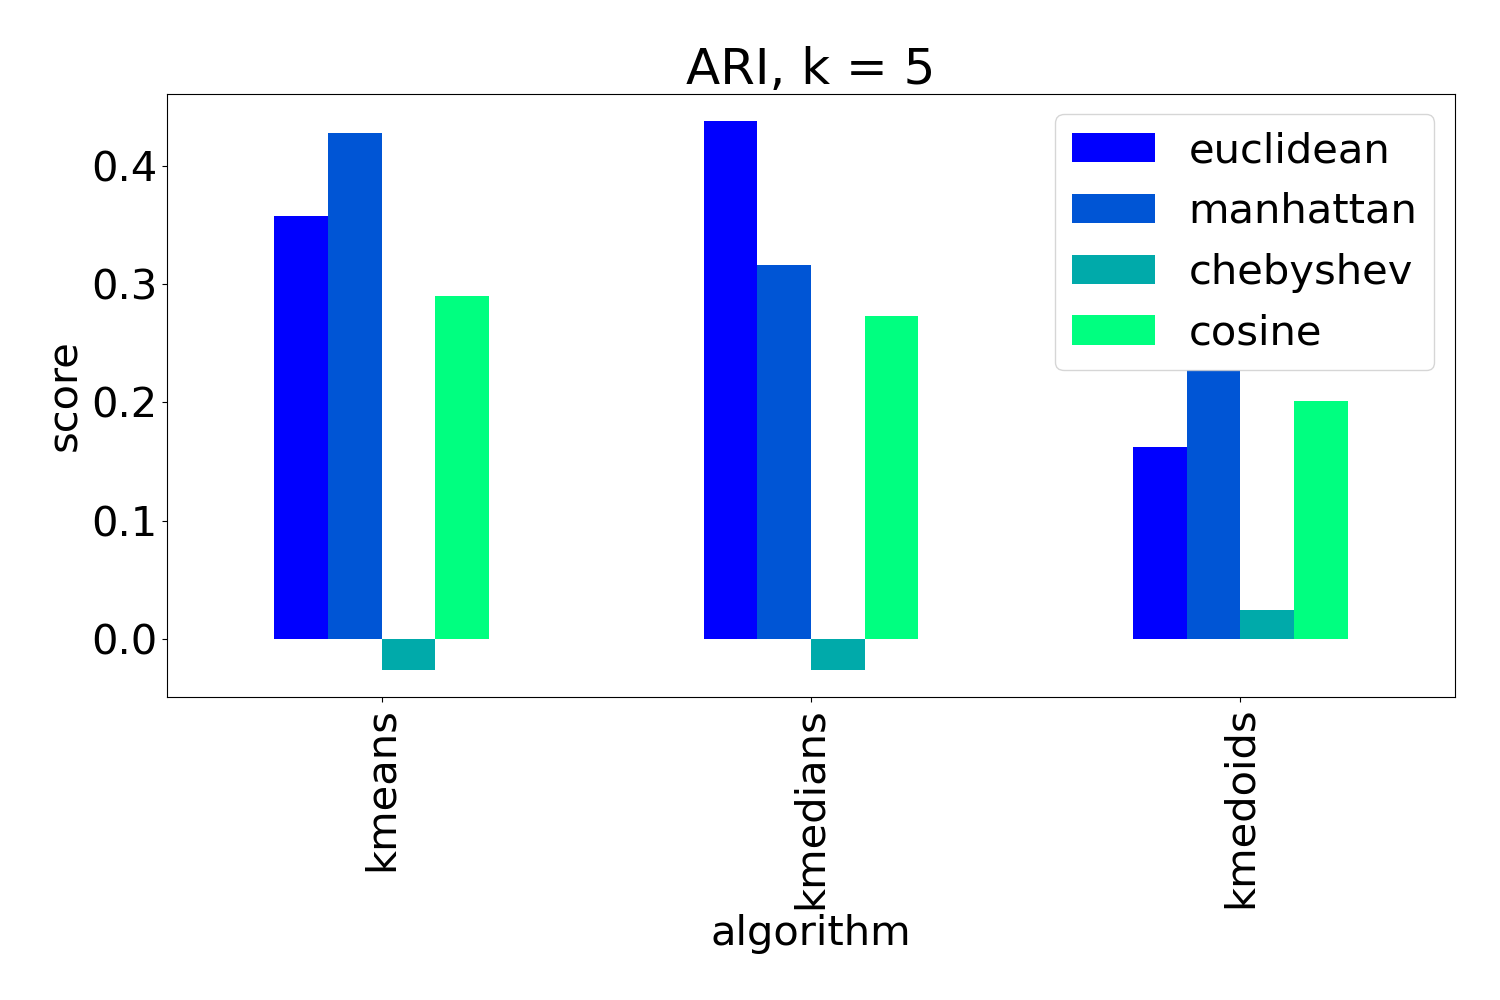
\includegraphics[width=0.45\textwidth]{../plots/housevotes/combined/ARI/algdist_for_given_k.png} }}%
	\qquad
	\subfloat[NMI ]{{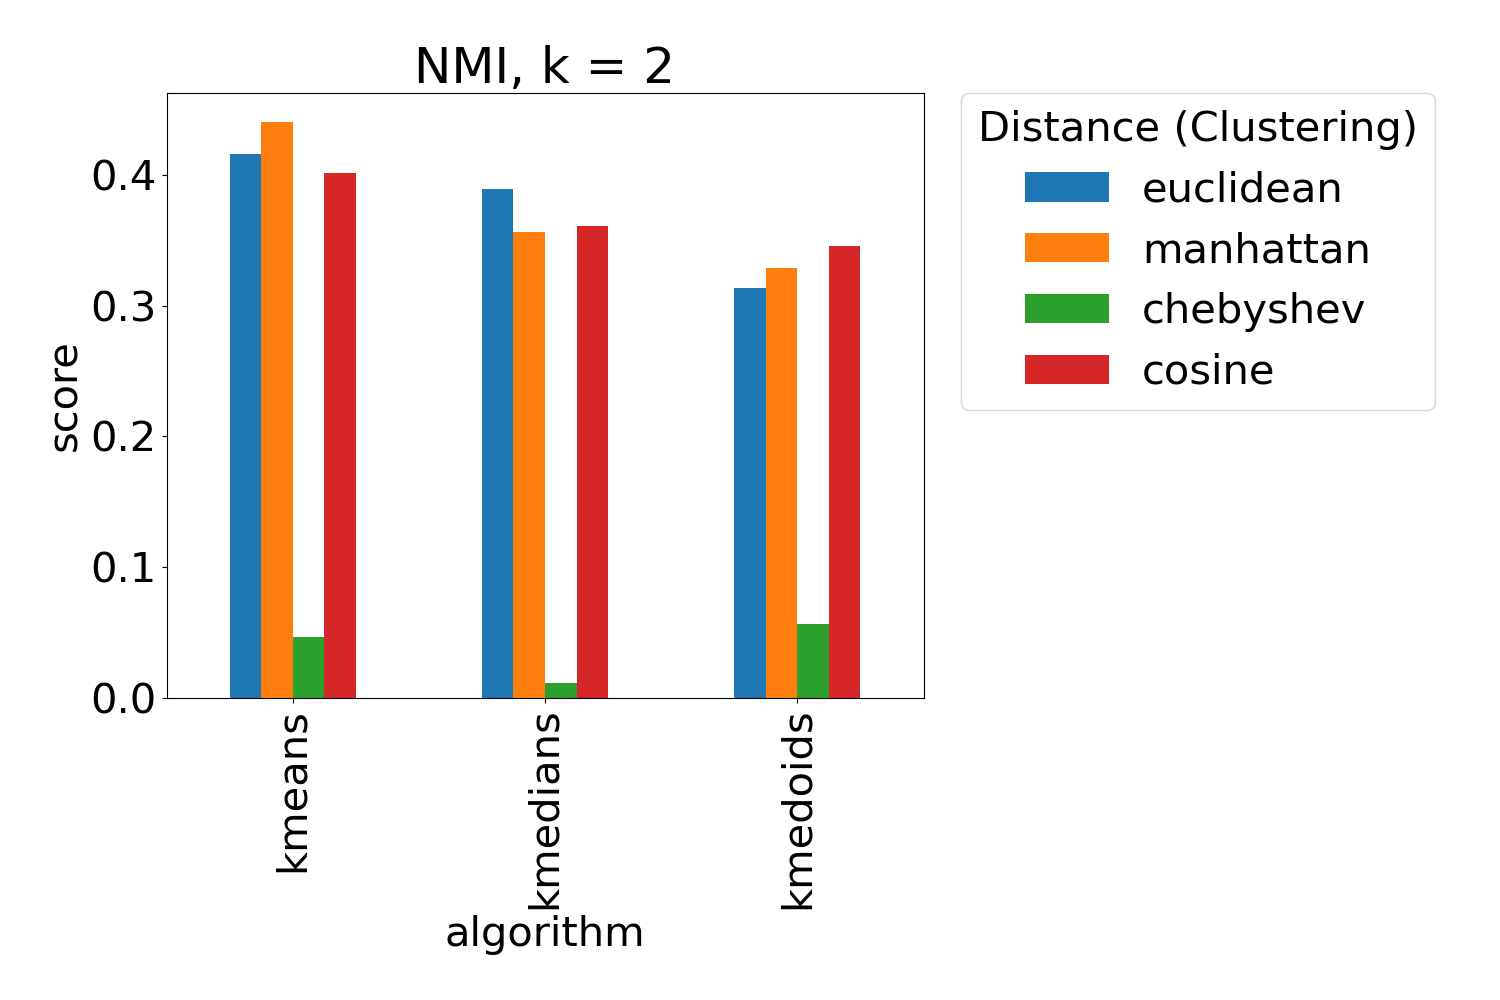
\includegraphics[width=0.45\textwidth]{../plots/housevotes/combined/NMI/algdist_for_given_k.png} }}%
	\qquad
	\subfloat[Completeness Score ]{{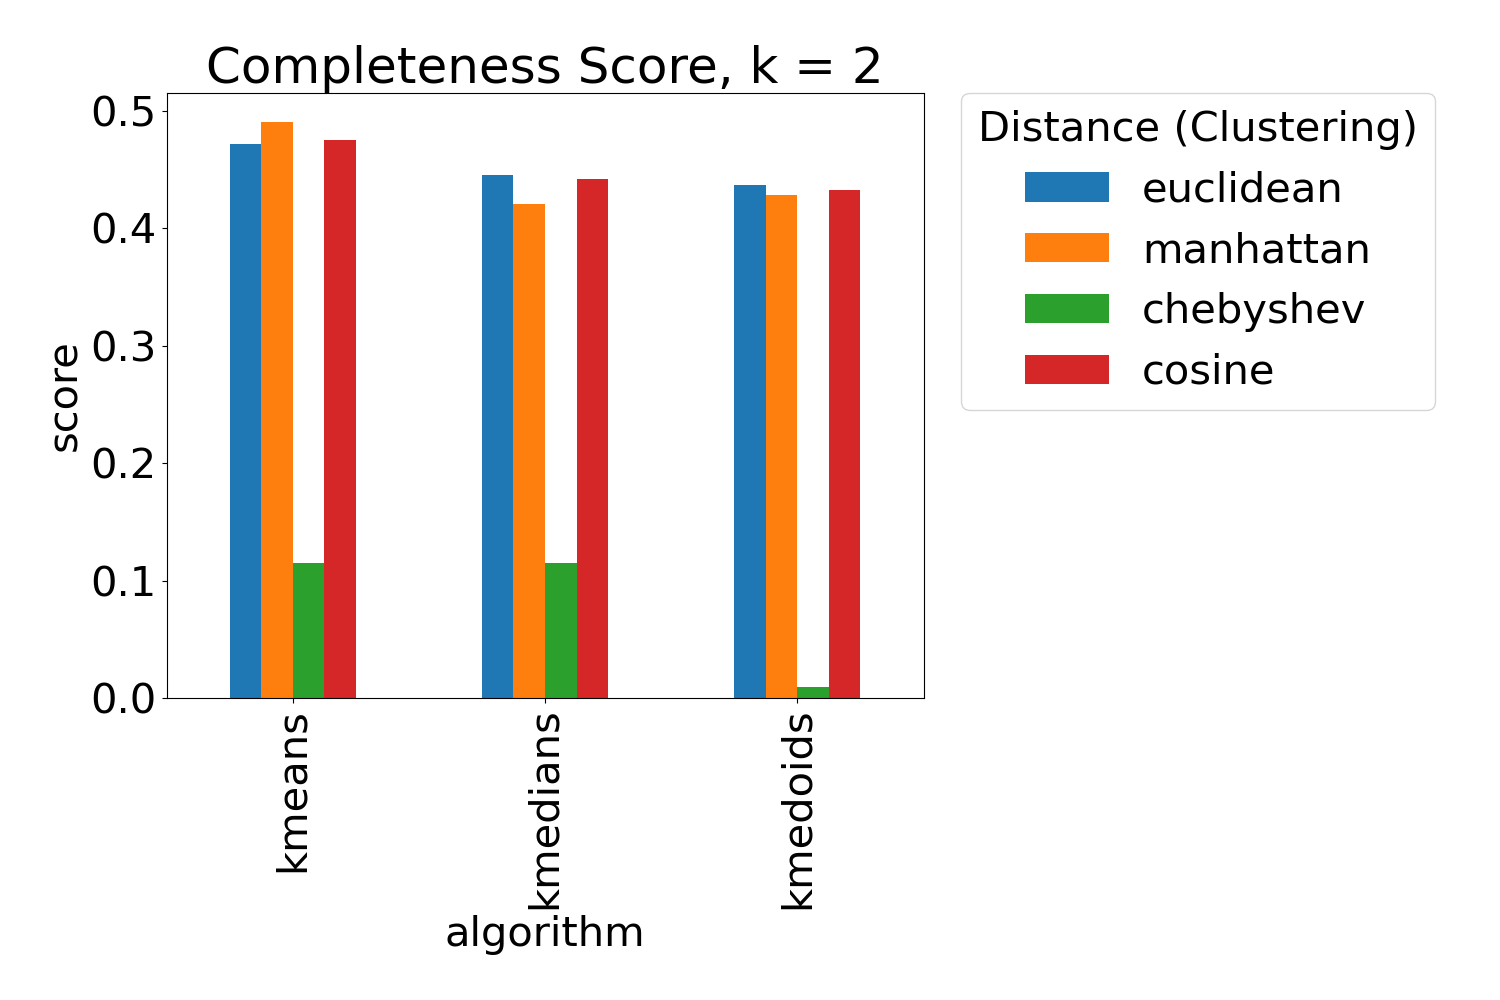
\includegraphics[width=0.45\textwidth]{../plots/housevotes/combined/Completeness Score/algdist_for_given_k.png} }}%
	\qquad
	\subfloat[Homogeneity Score ]{{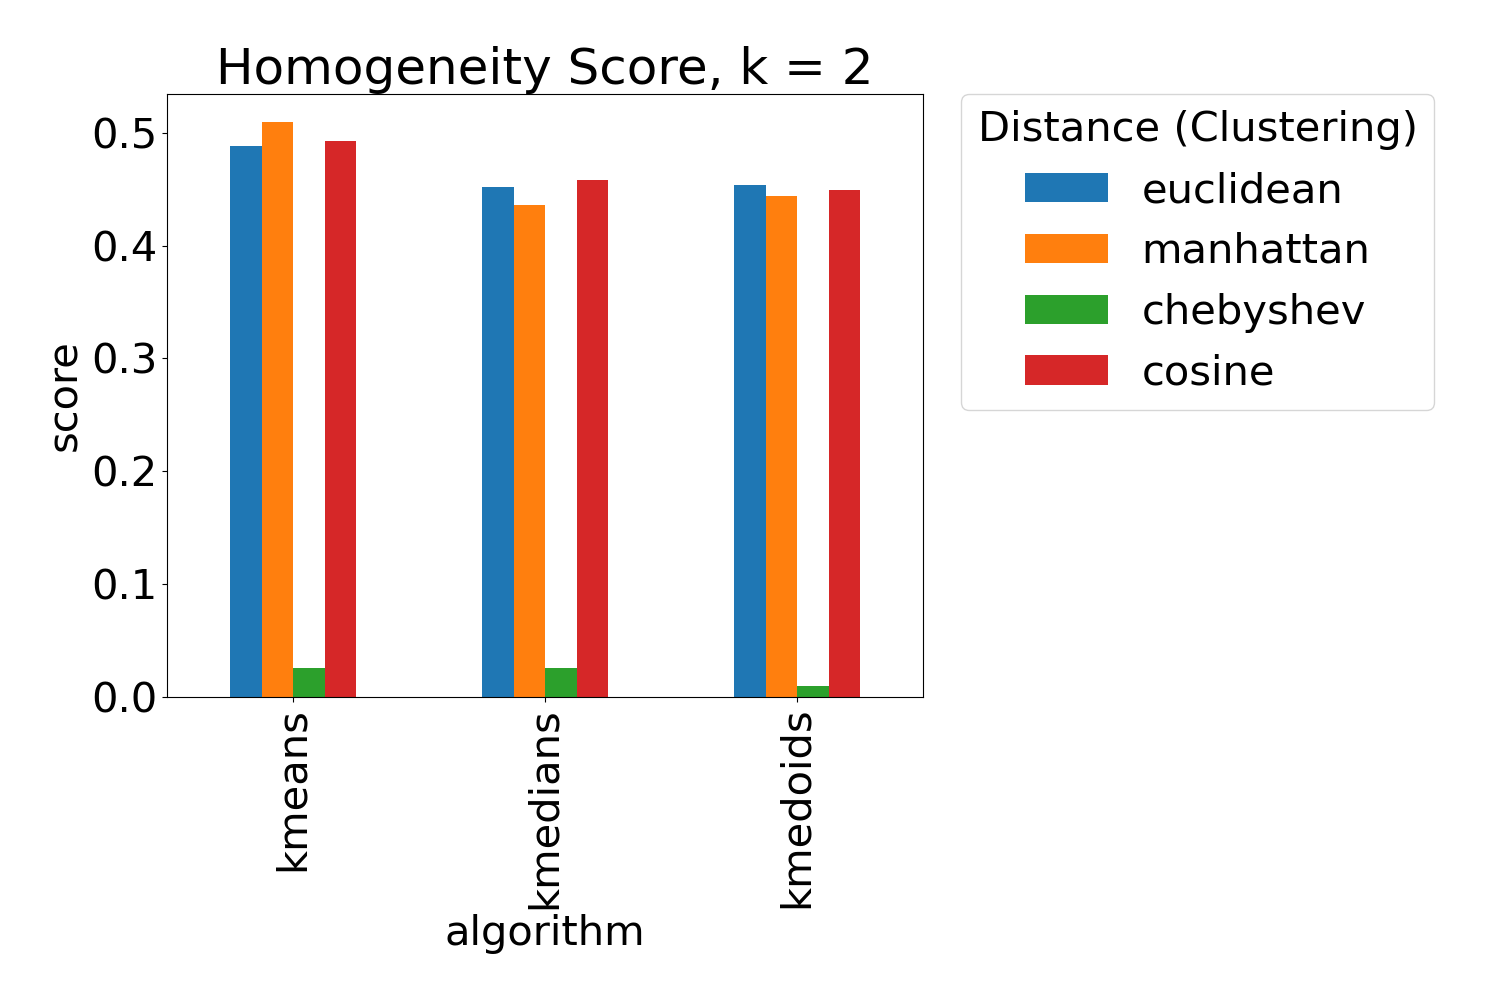
\includegraphics[width=0.45\textwidth]{../plots/housevotes/combined/Homogeneity Score/algdist_for_given_k.png} }}%
	\qquad
	\subfloat[Silhouette Score ]{{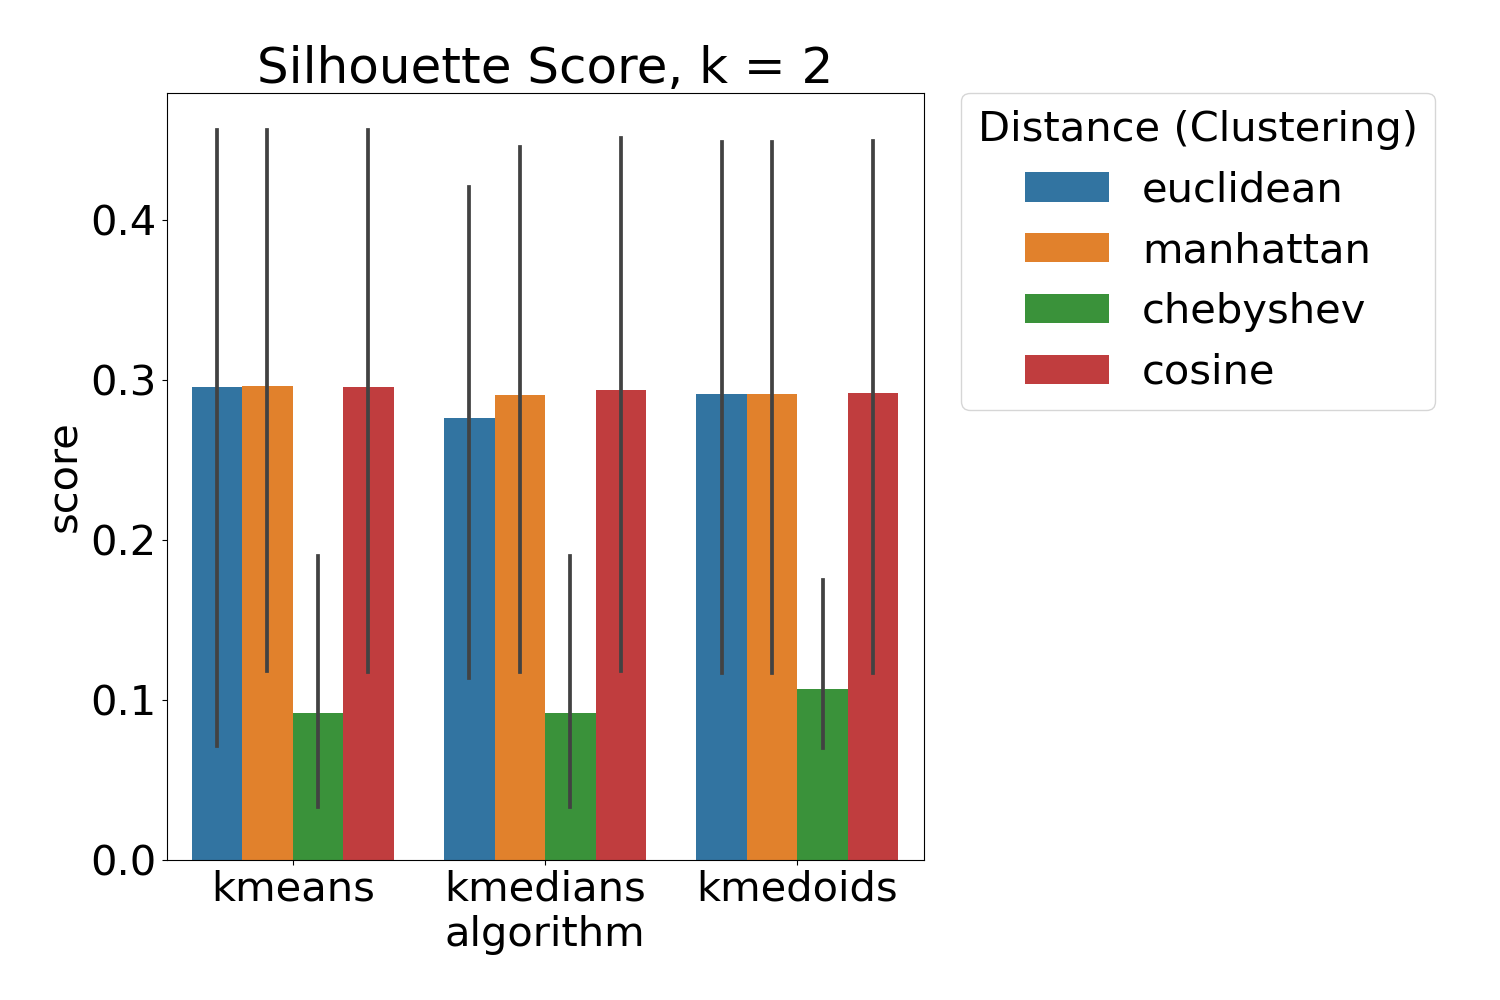
\includegraphics[width=0.45\textwidth]{../plots/housevotes/combined/Silhouette Score/algdist_for_given_k.png} }}%
	
	\caption{Comparison of clustering scores for Housevotes dataset (given k=2)}%
\end{figure}

To estimate the number of meaningful clusters (clusterings with highest index scores) in the datasets and test the robustness of different distance measures we compared scorings as a function of k. \\

\begin{figure}[H]
	\centering
	\subfloat[ARI ]{{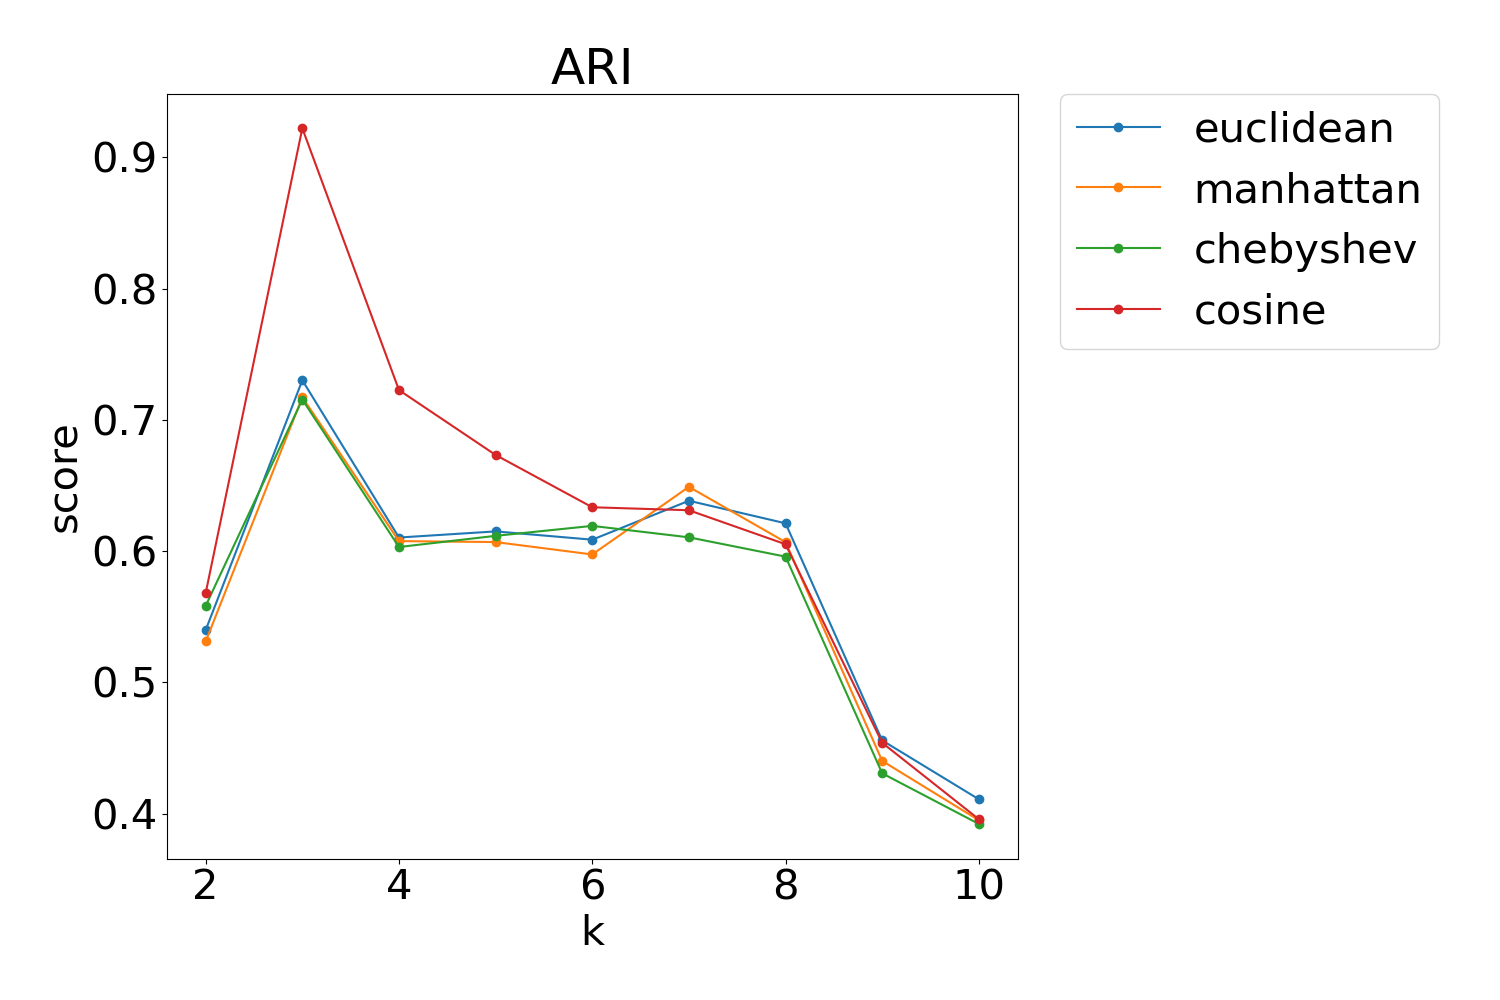
\includegraphics[width=0.45\textwidth]{../plots/iris/kmeans/ARI/k_1to10.png} }}%
	\qquad
	\subfloat[NMI ]{{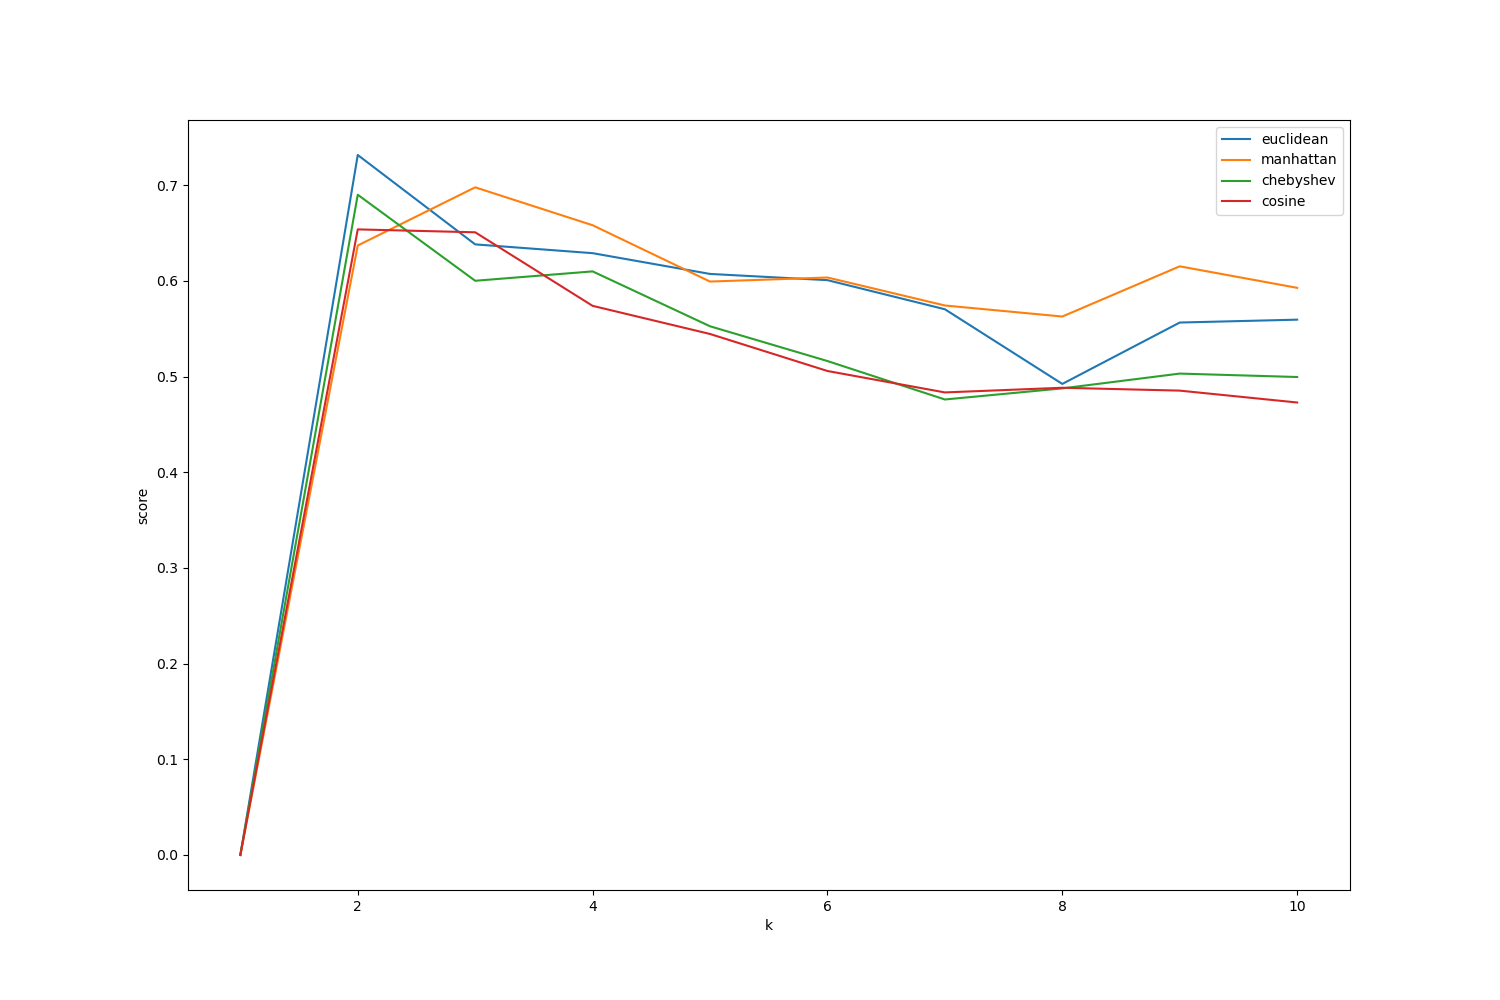
\includegraphics[width=0.45\textwidth]{../plots/iris/kmeans/NMI/k_1to10.png} }}%
	\qquad
	\subfloat[Completeness Score ]{{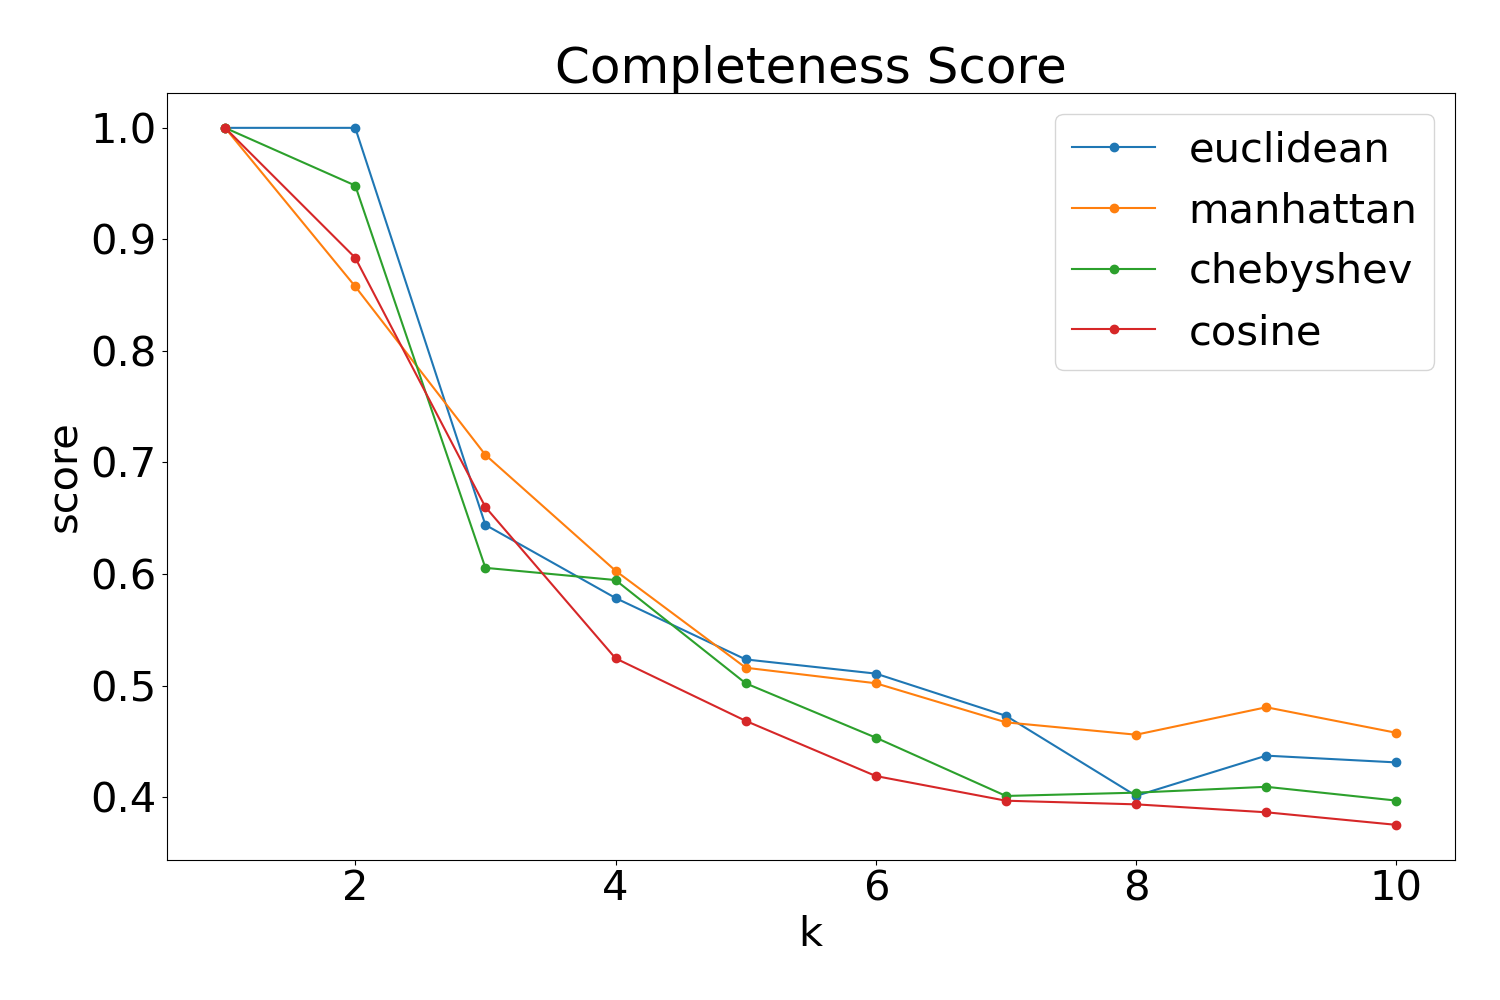
\includegraphics[width=0.45\textwidth]{../plots/iris/kmeans/Completeness Score/k_1to10.png} }}%
	\qquad
	\subfloat[Homogeneity Score ]{{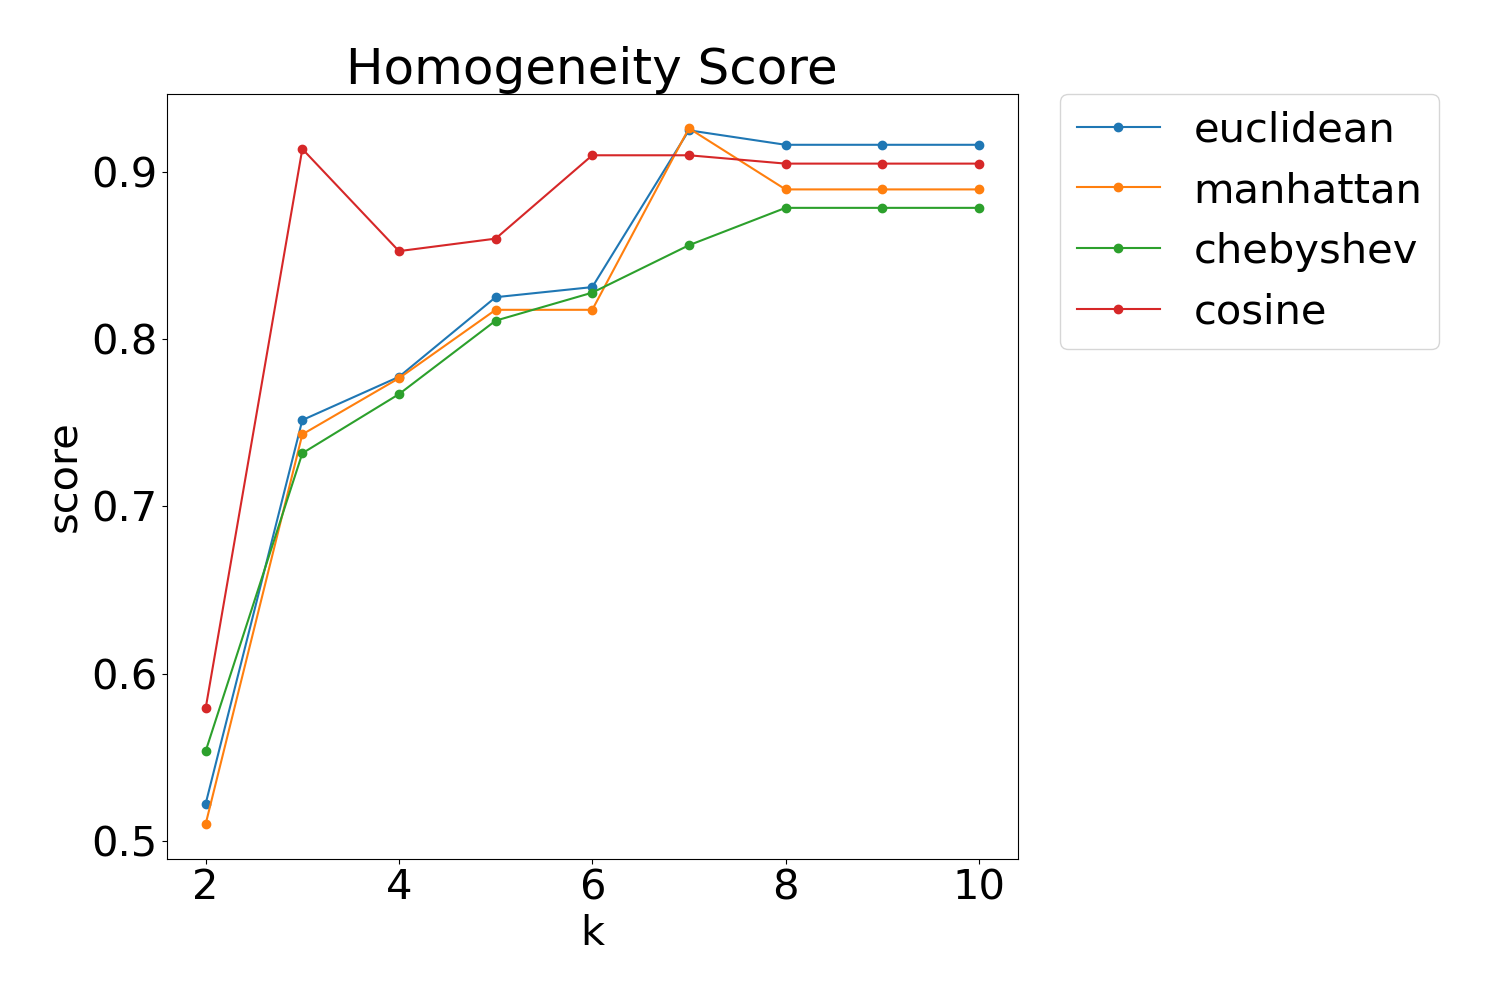
\includegraphics[width=0.45\textwidth]{../plots/iris/kmeans/Homogeneity Score/k_1to10.png} }}%
	\qquad
	\subfloat[Silhouette Score ]{{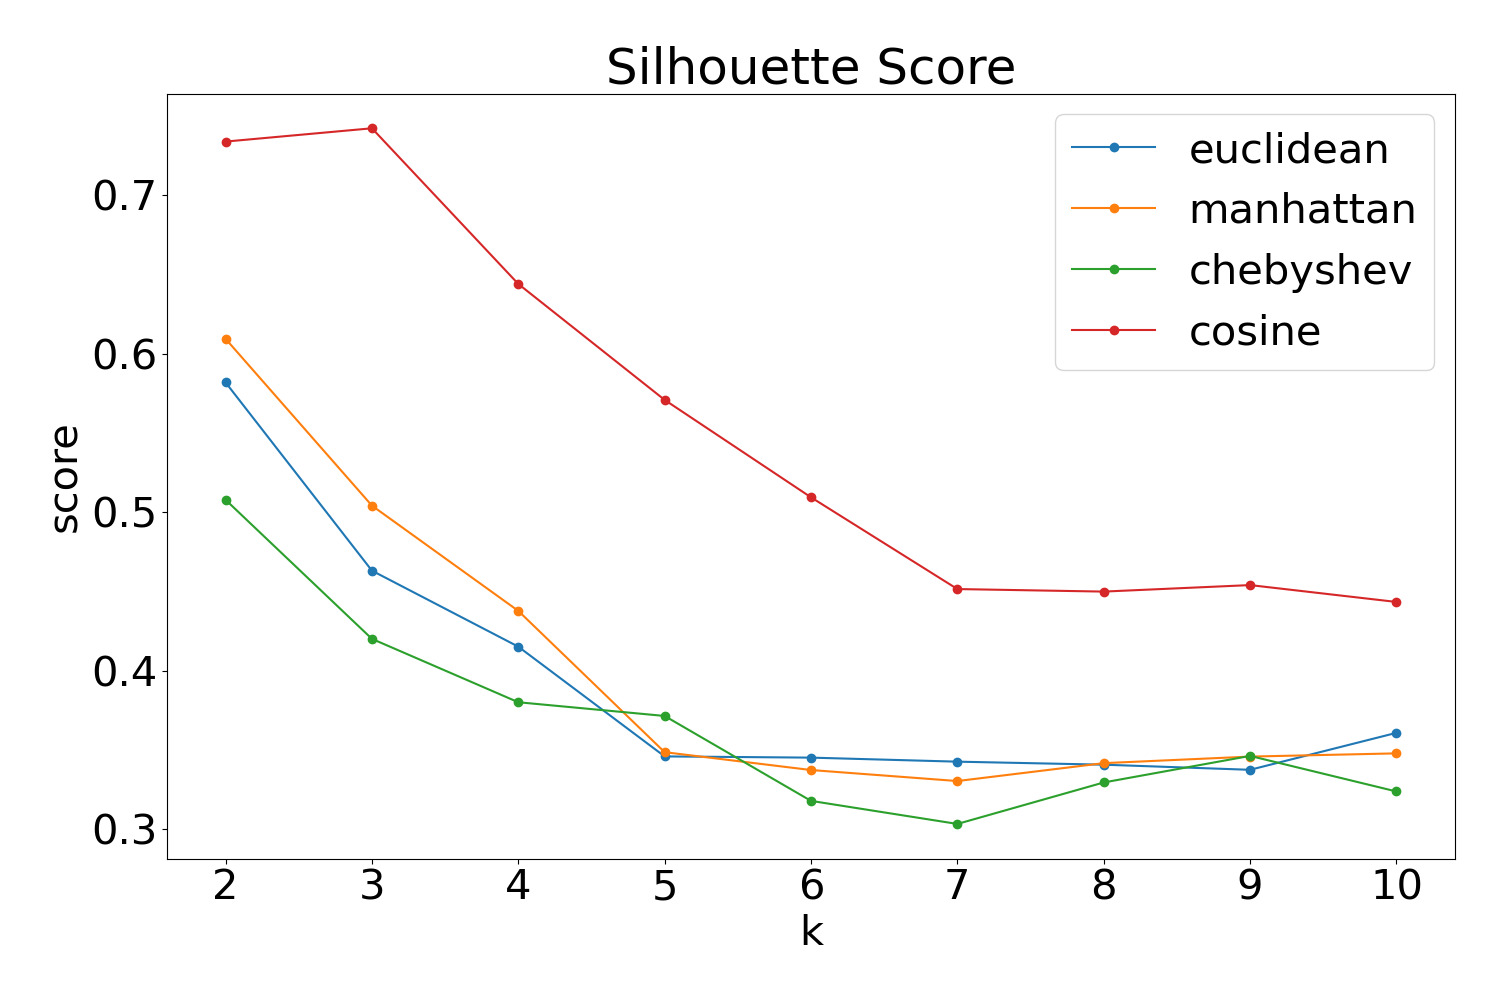
\includegraphics[width=1\textwidth]{../plots/iris/kmeans/Silhouette Score/k_1to10.png} }}%
	
	\caption{Comparison of clustering scores for kmeans-clustering on Iris dataset}%
\end{figure}

\begin{figure}[H]
	\centering
	\subfloat[ARI ]{{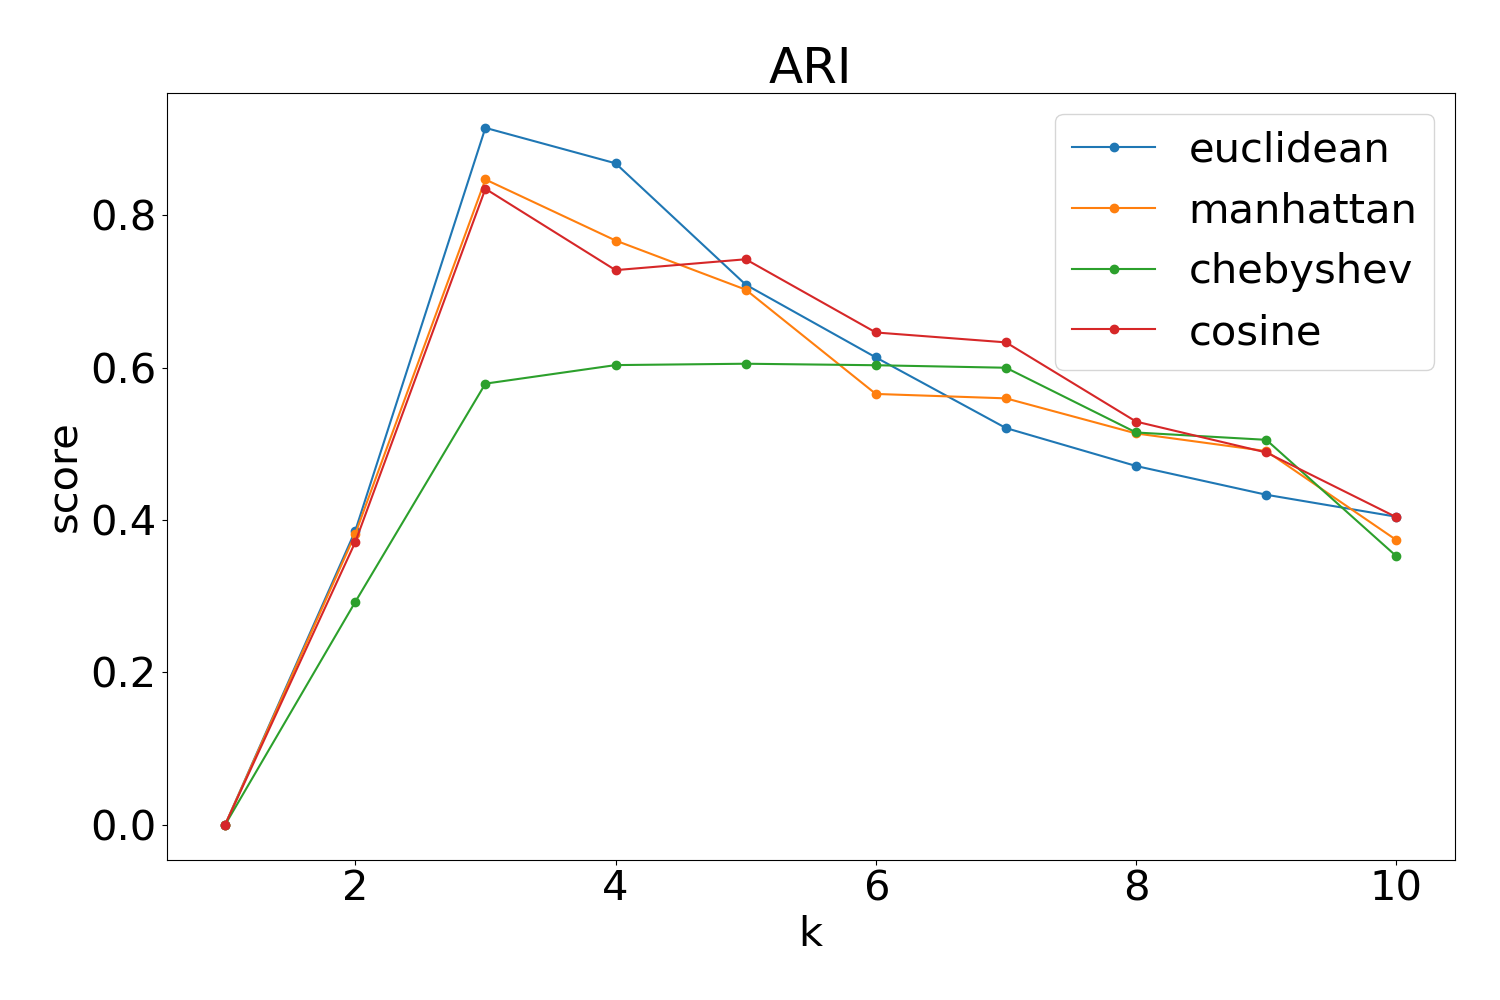
\includegraphics[width=0.45\textwidth]{../plots/wine/kmeans/ARI/k_1to10.png} }}%
	\qquad
	\subfloat[NMI ]{{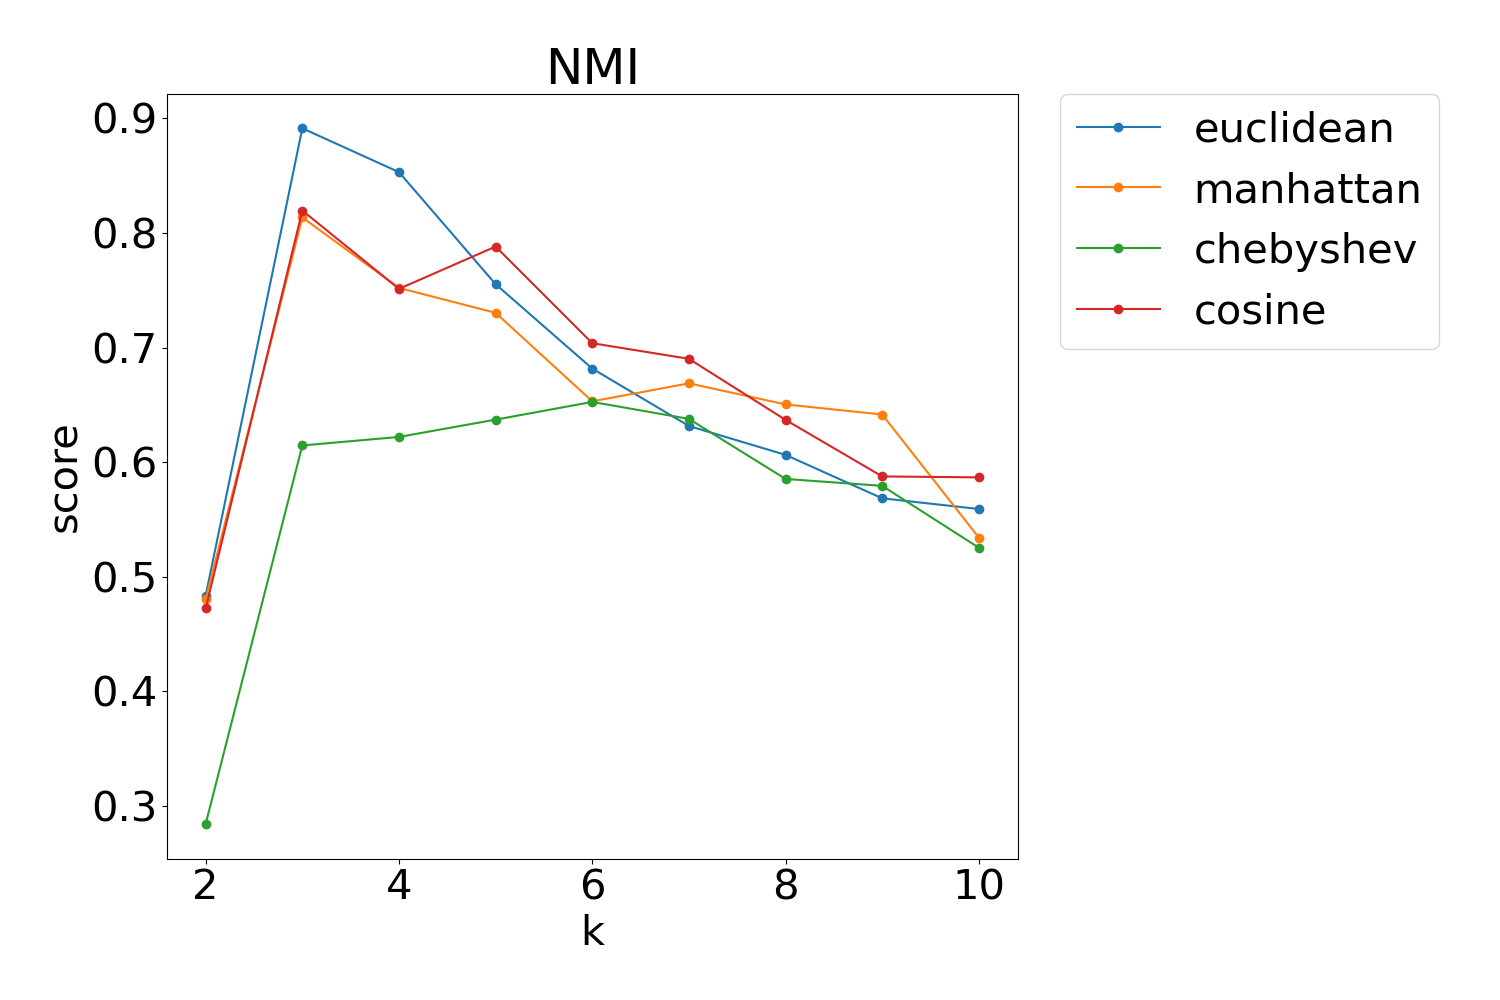
\includegraphics[width=0.45\textwidth]{../plots/wine/kmeans/NMI/k_1to10.png} }}%
	\qquad
	\subfloat[Completeness Score ]{{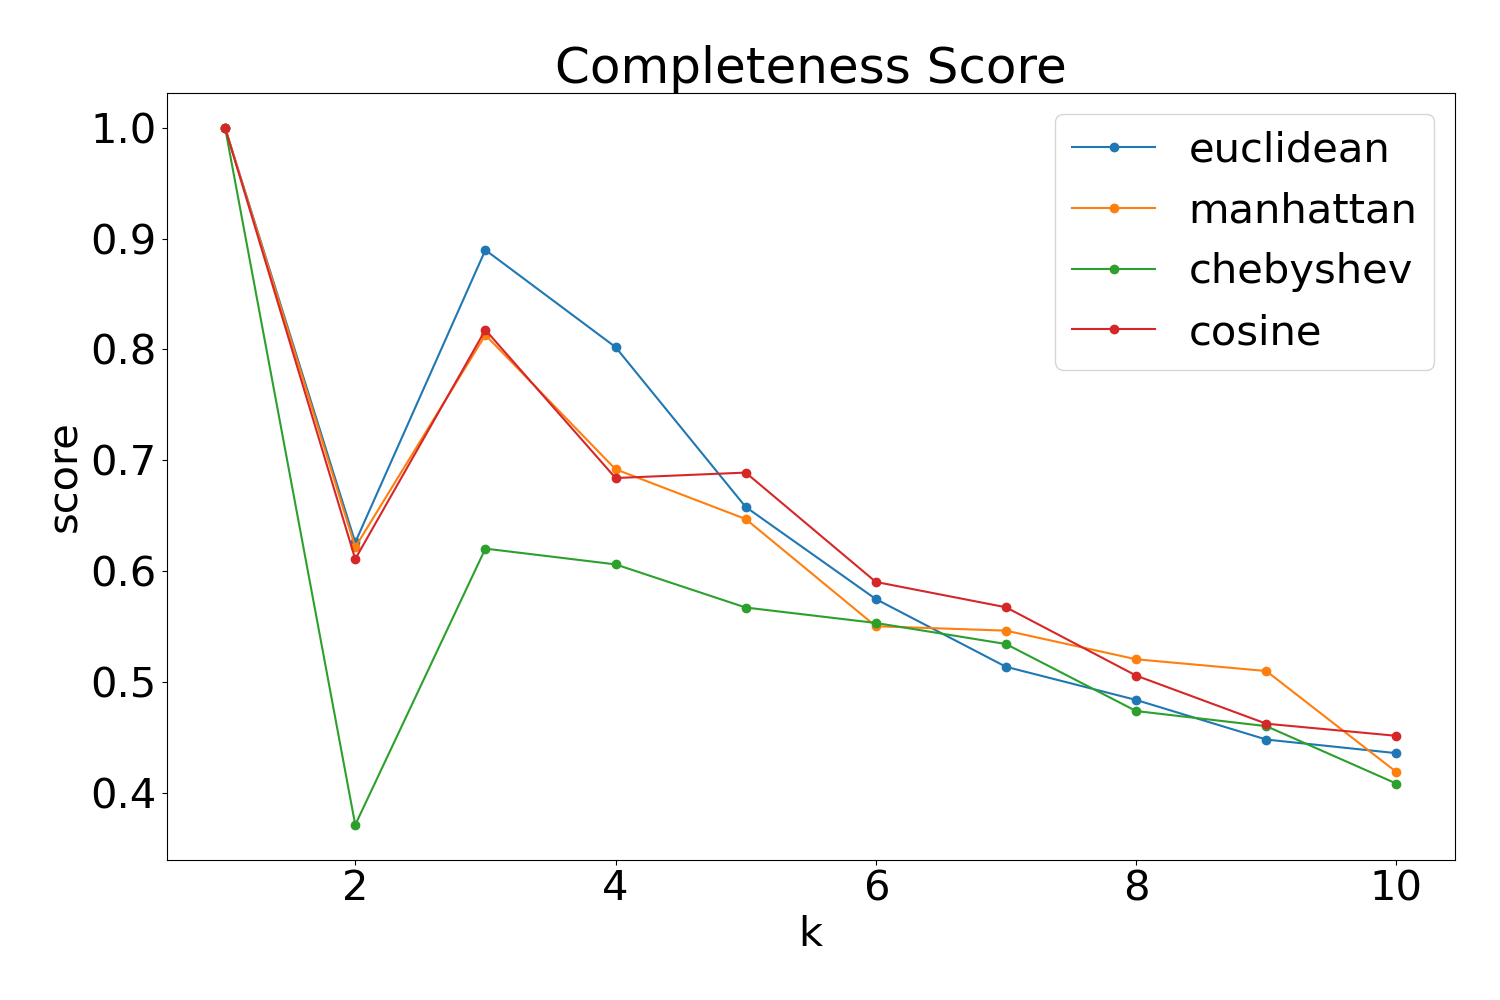
\includegraphics[width=0.45\textwidth]{../plots/wine/kmeans/Completeness Score/k_1to10.png} }}%
	\qquad
	\subfloat[Homogeneity Score ]{{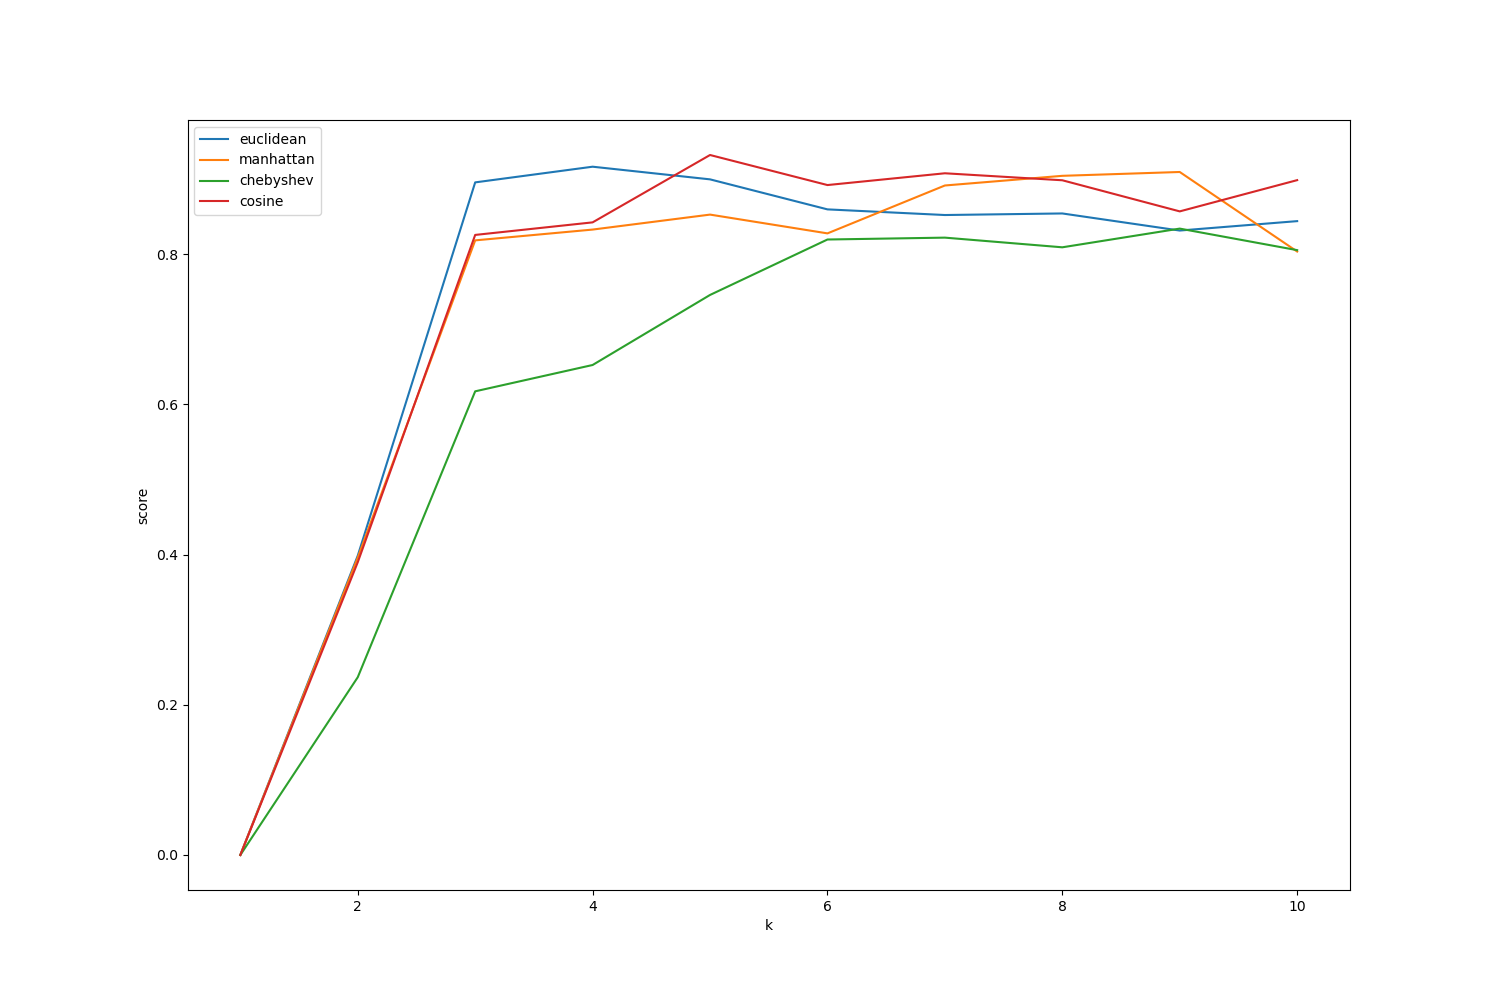
\includegraphics[width=0.45\textwidth]{../plots/wine/kmeans/Homogeneity Score/k_1to10.png} }}%
	\qquad
	\subfloat[Silhouette Score ]{{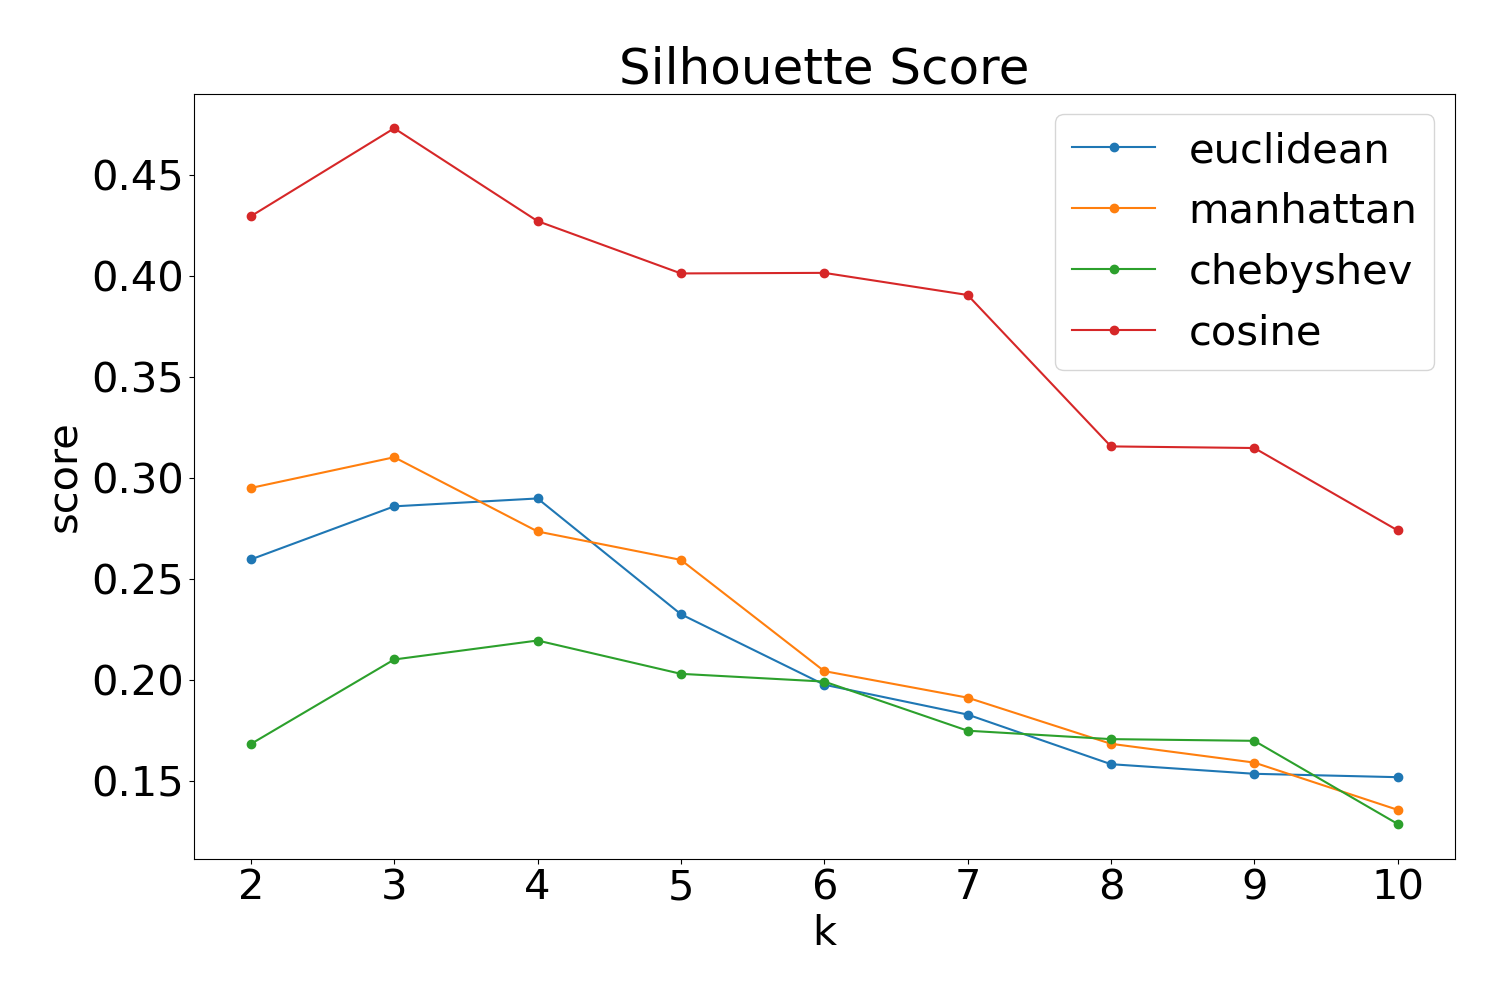
\includegraphics[width=1\textwidth]{../plots/wine/kmeans/Silhouette Score/k_1to10.png} }}%
	
	\caption{Comparison of clustering scores for kmeans-clustering on Wine dataset}%
\end{figure}

\begin{figure}[H]
	\centering
	\subfloat[Silhouette Score ]{{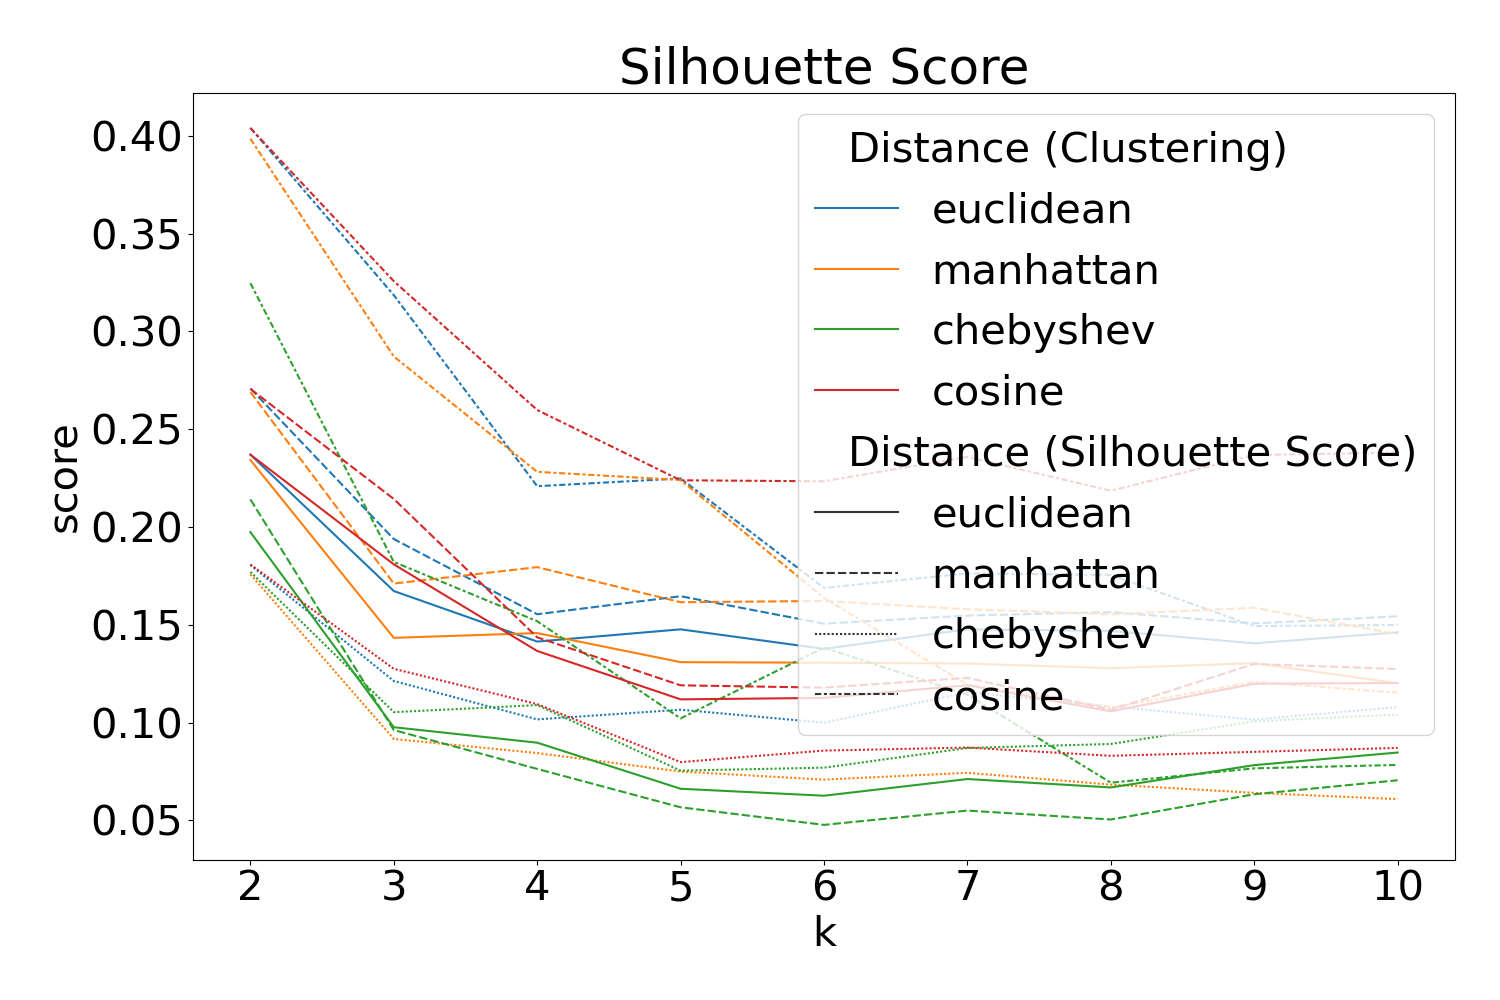
\includegraphics[width=1\textwidth]{../plots/diabetes/kmeans/Silhouette Score/k_1to10.png} }}%
	
	\caption{Comparison of clustering scores for kmeans-clustering on Diabetes dataset}%
\end{figure}

\begin{figure}[H]
	\centering
	\subfloat[ARI ]{{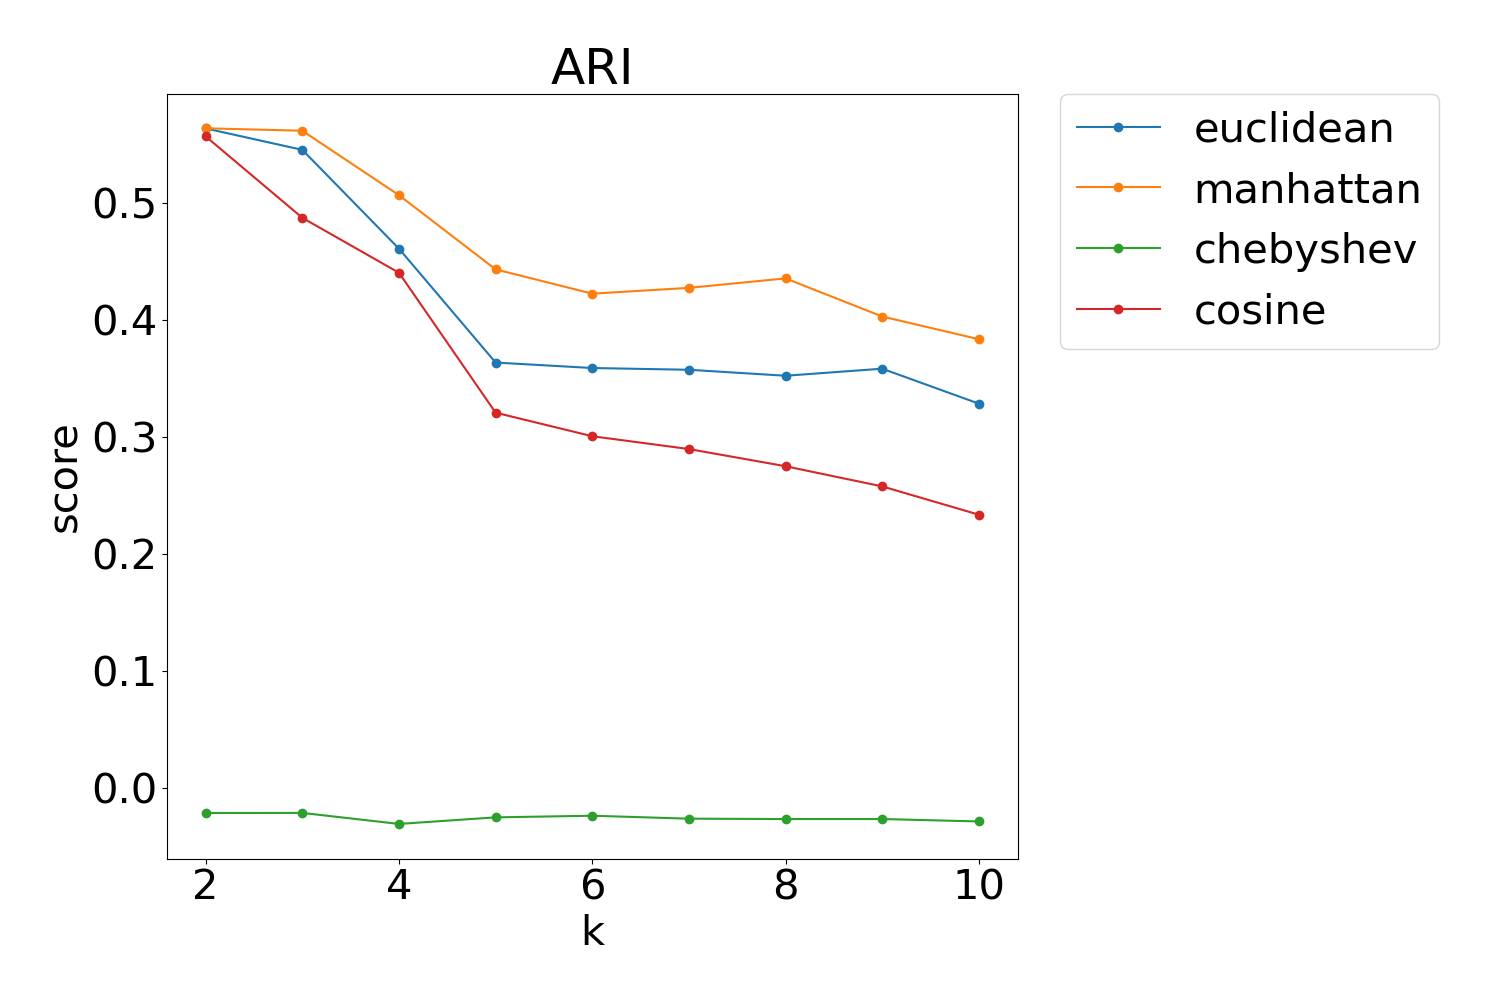
\includegraphics[width=0.45\textwidth]{../plots/housevotes/kmeans/ARI/k_1to10.png} }}%
	\qquad
	\subfloat[NMI ]{{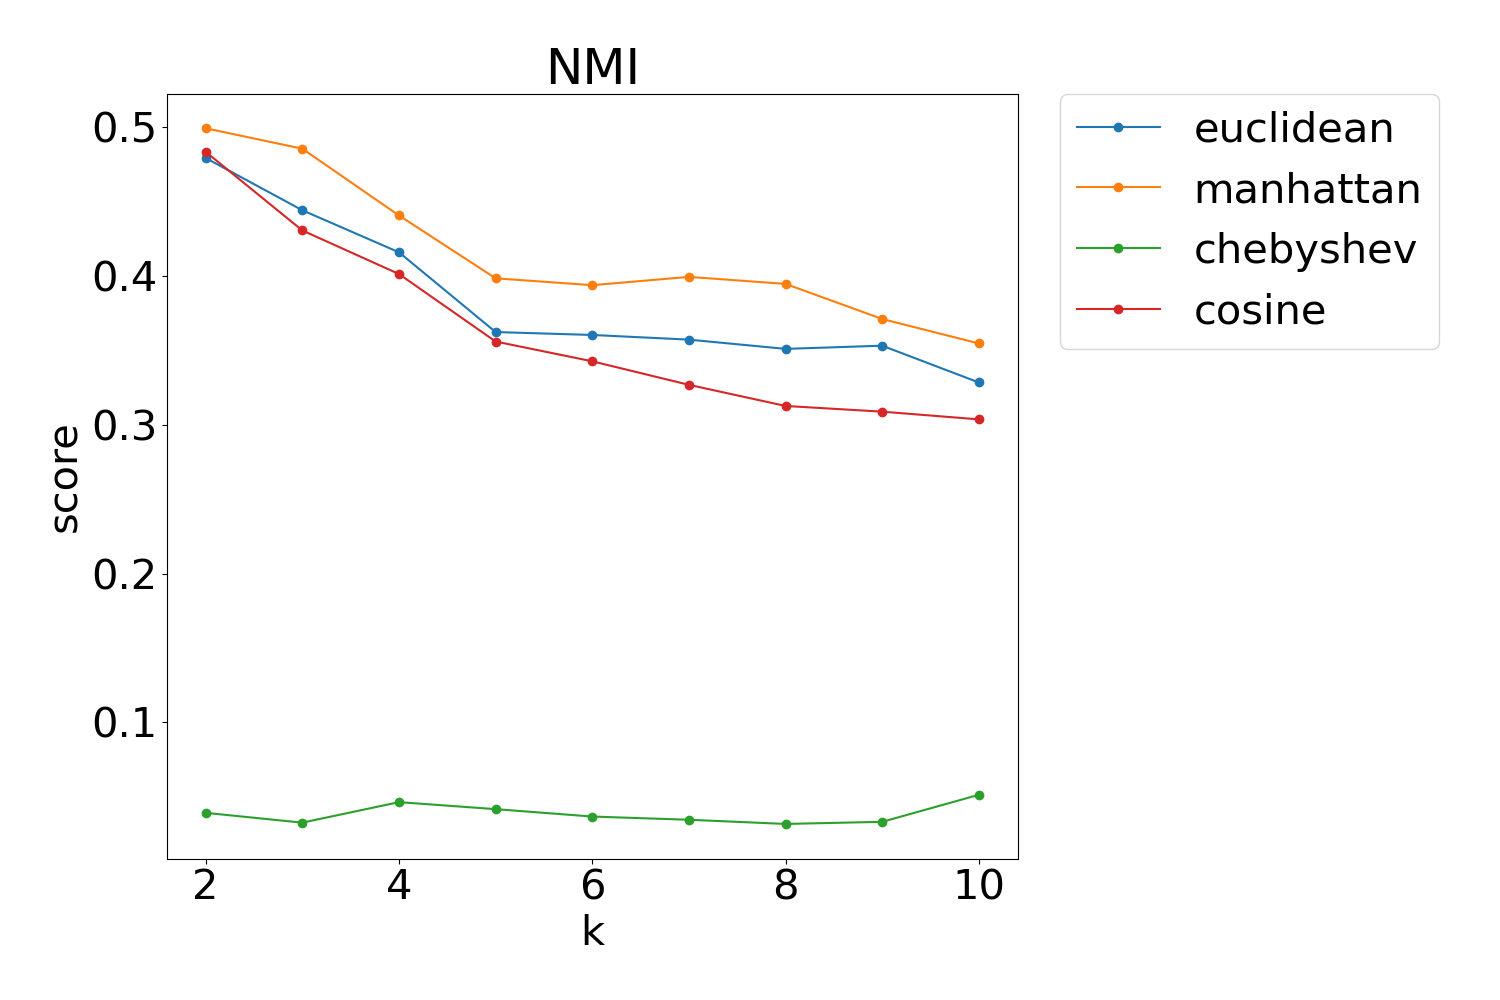
\includegraphics[width=0.45\textwidth]{../plots/housevotes/kmeans/NMI/k_1to10.png} }}%
	\qquad
	\subfloat[Completeness Score ]{{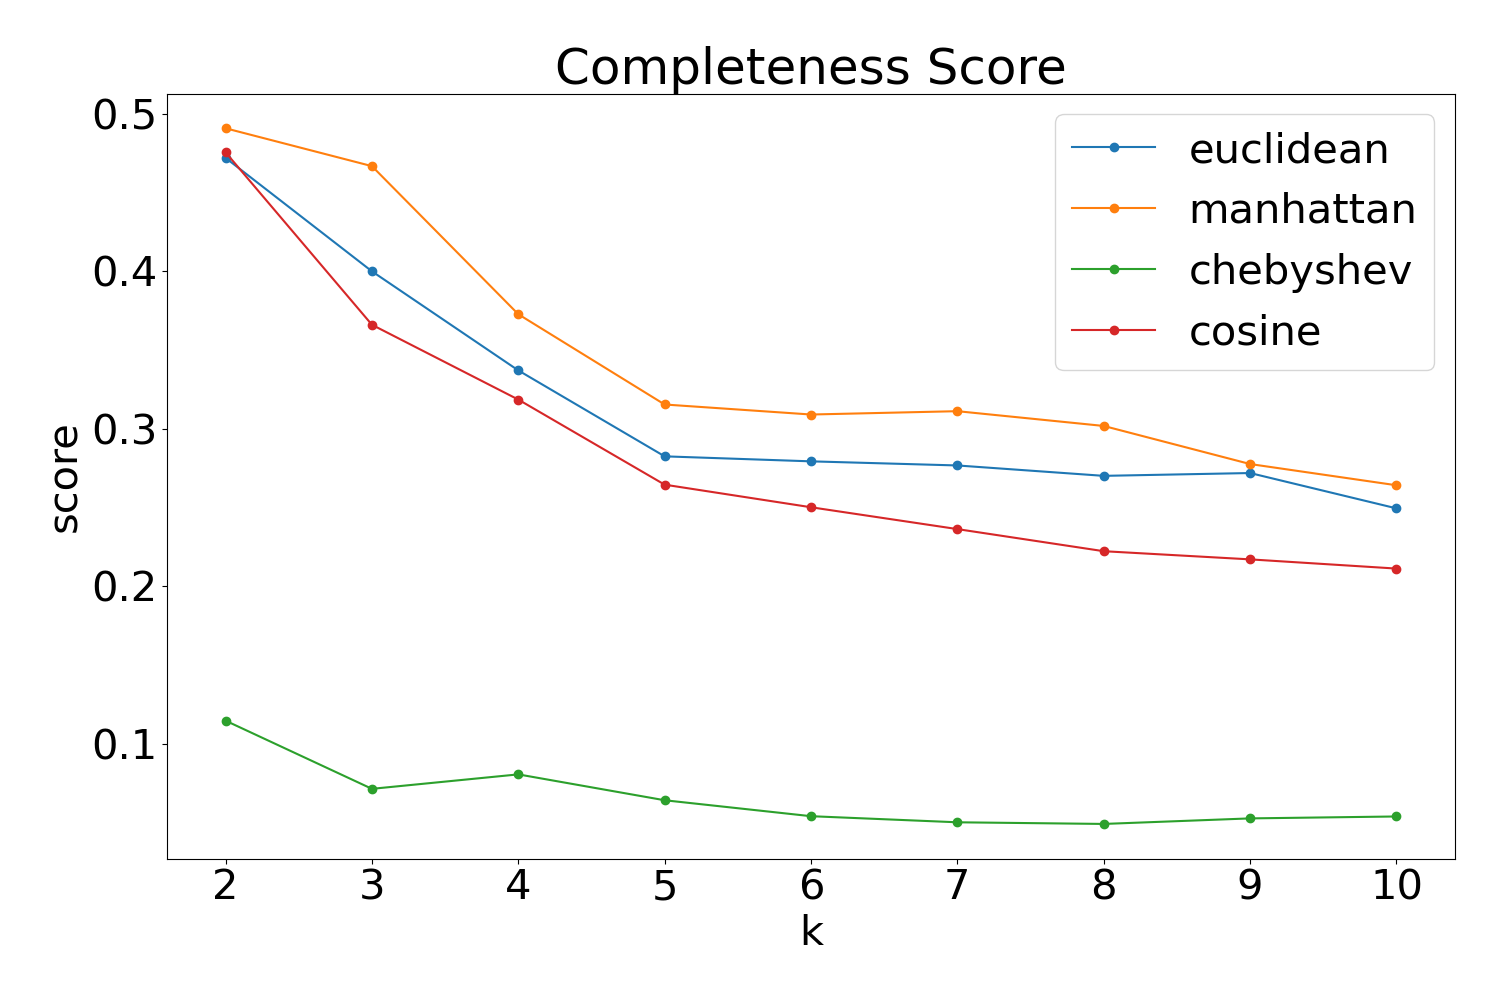
\includegraphics[width=0.45\textwidth]{../plots/housevotes/kmeans/Completeness Score/k_1to10.png} }}%
	\qquad
	\subfloat[Homogeneity Score ]{{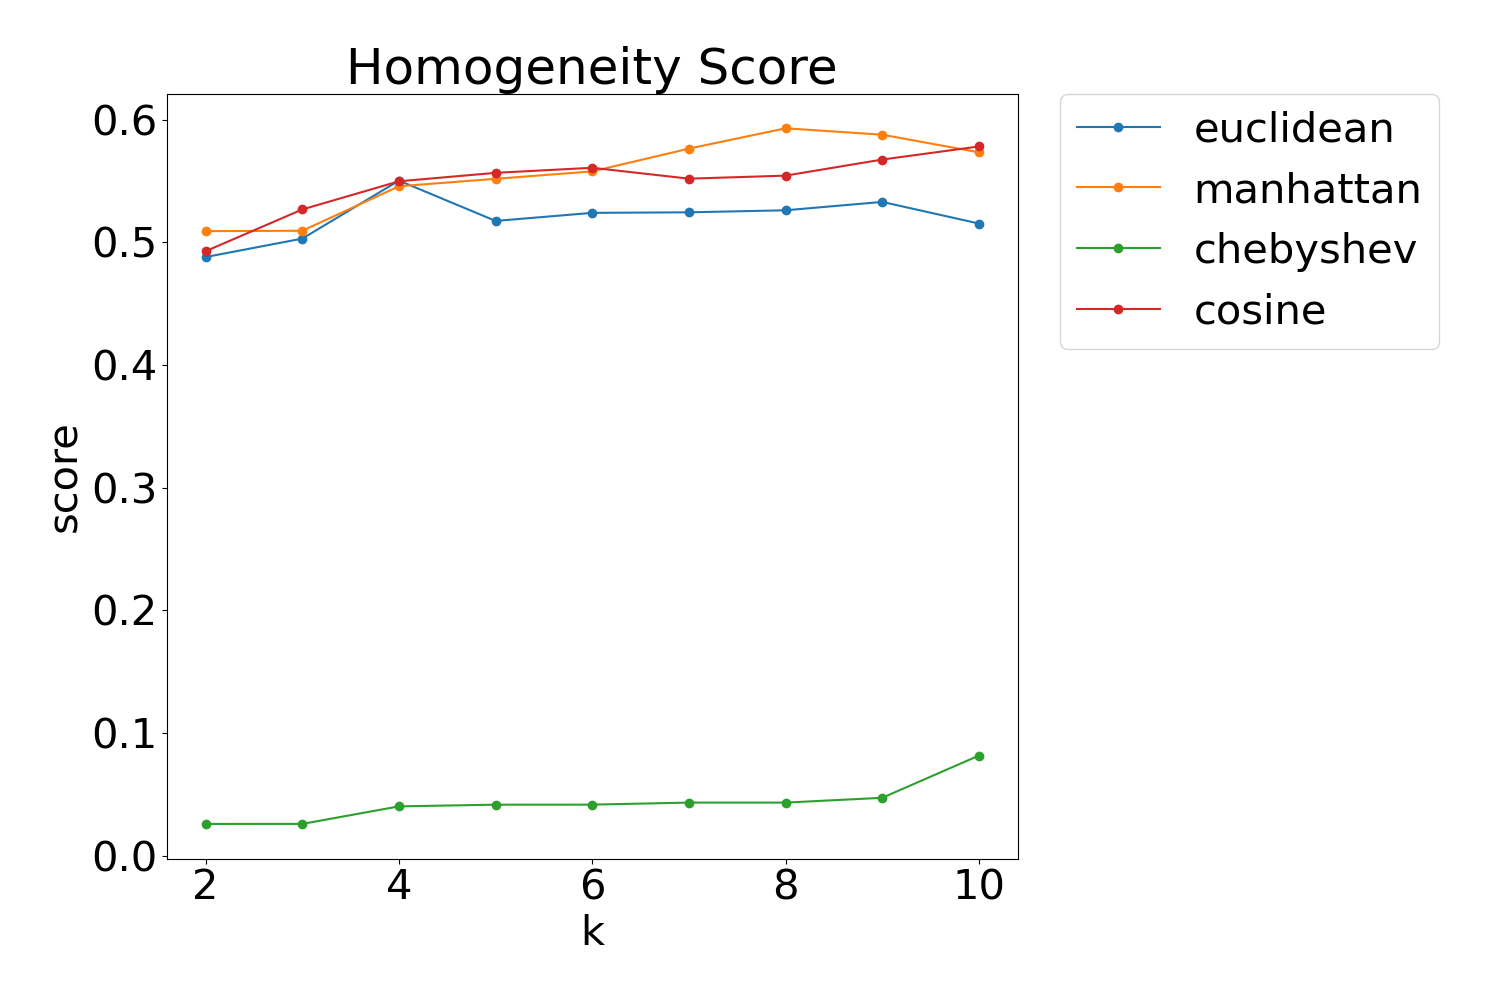
\includegraphics[width=0.45\textwidth]{../plots/housevotes/kmeans/Homogeneity Score/k_1to10.png} }}%
	\qquad
	\subfloat[Silhouette Score ]{{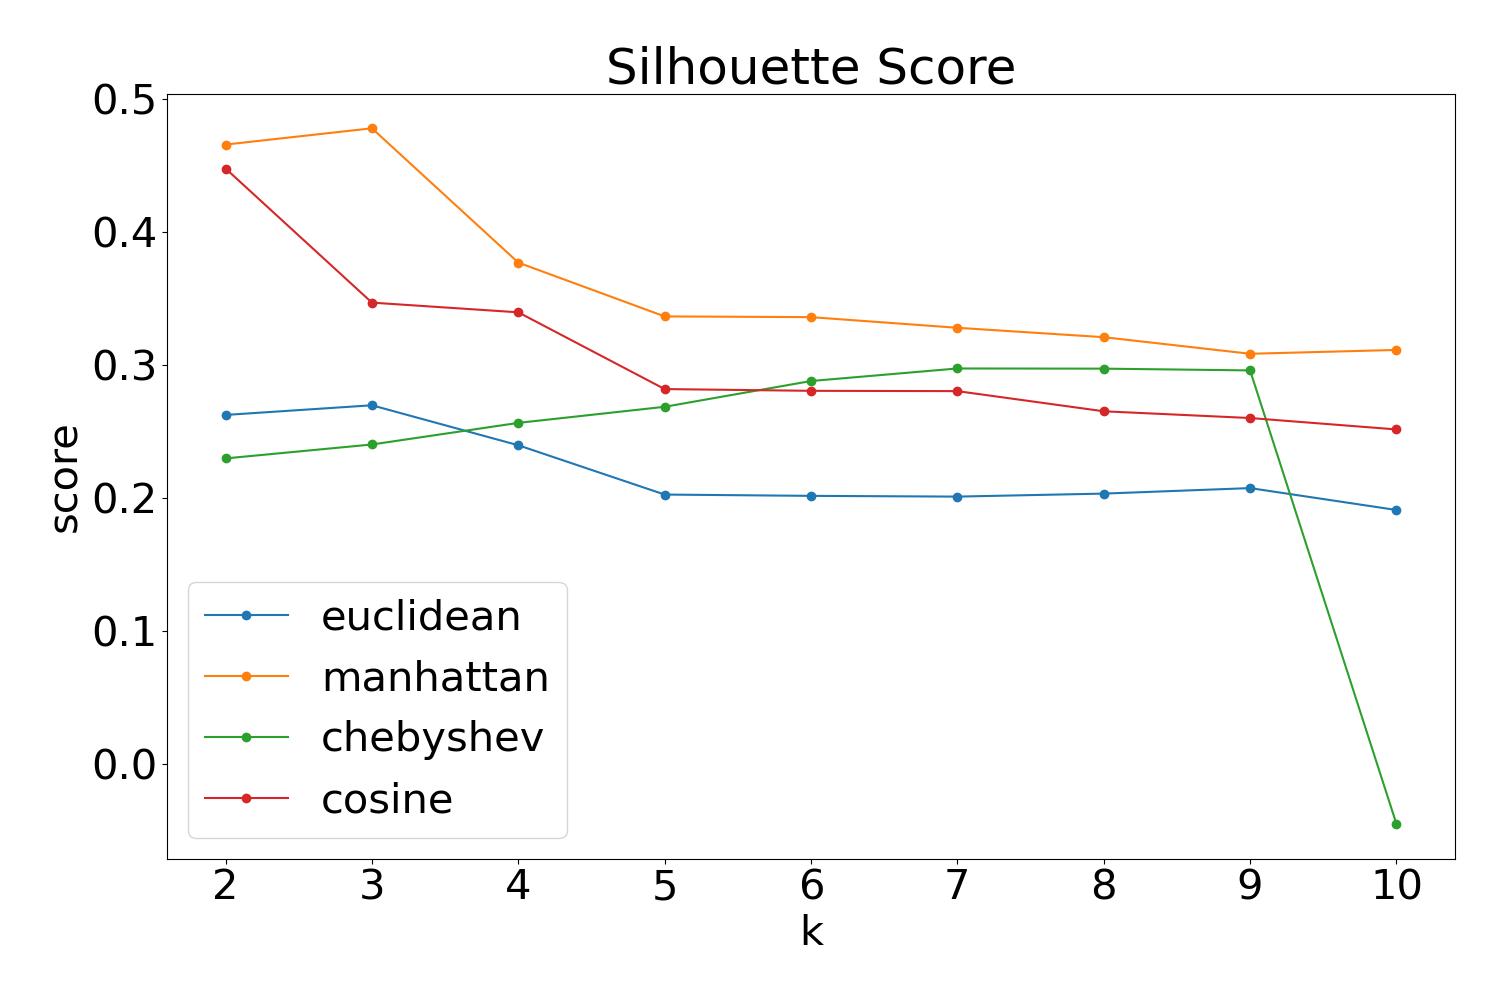
\includegraphics[width=1\textwidth]{../plots/housevotes/kmeans/Silhouette Score/k_1to10.png} }}%
	
	\caption{Comparison of clustering scores for kmeans-clustering on Housevotes dataset}%
\end{figure}

\begin{figure}[H]
	\centering
	\subfloat[ARI ]{{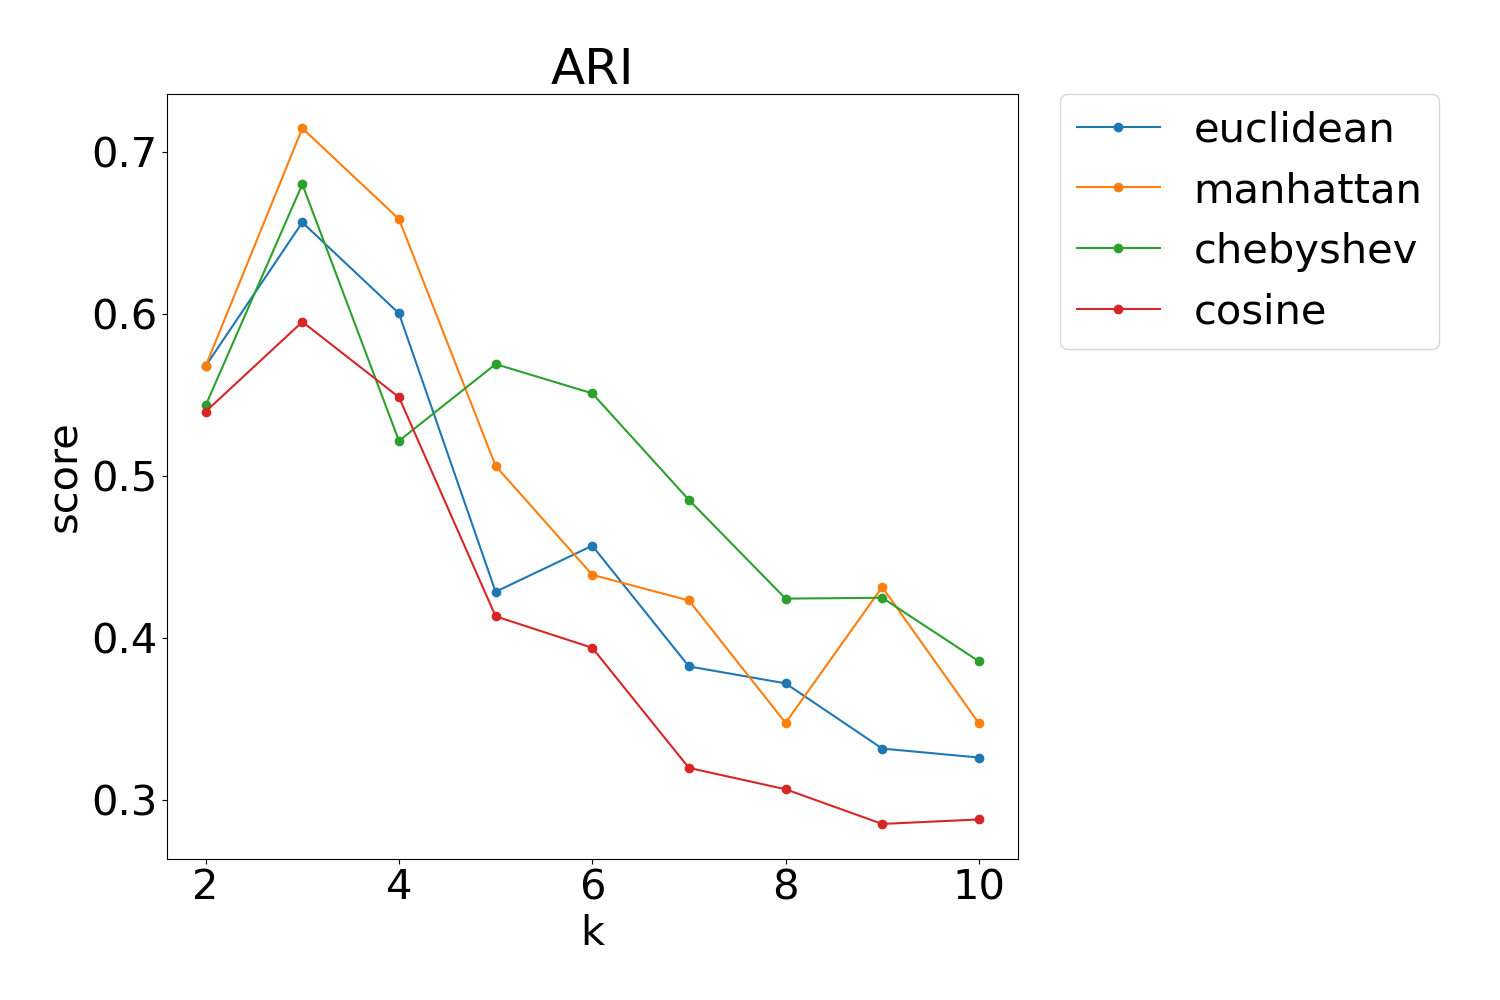
\includegraphics[width=0.45\textwidth]{../plots/iris/kmedians/ARI/k_1to10.png} }}%
	\qquad
	\subfloat[NMI ]{{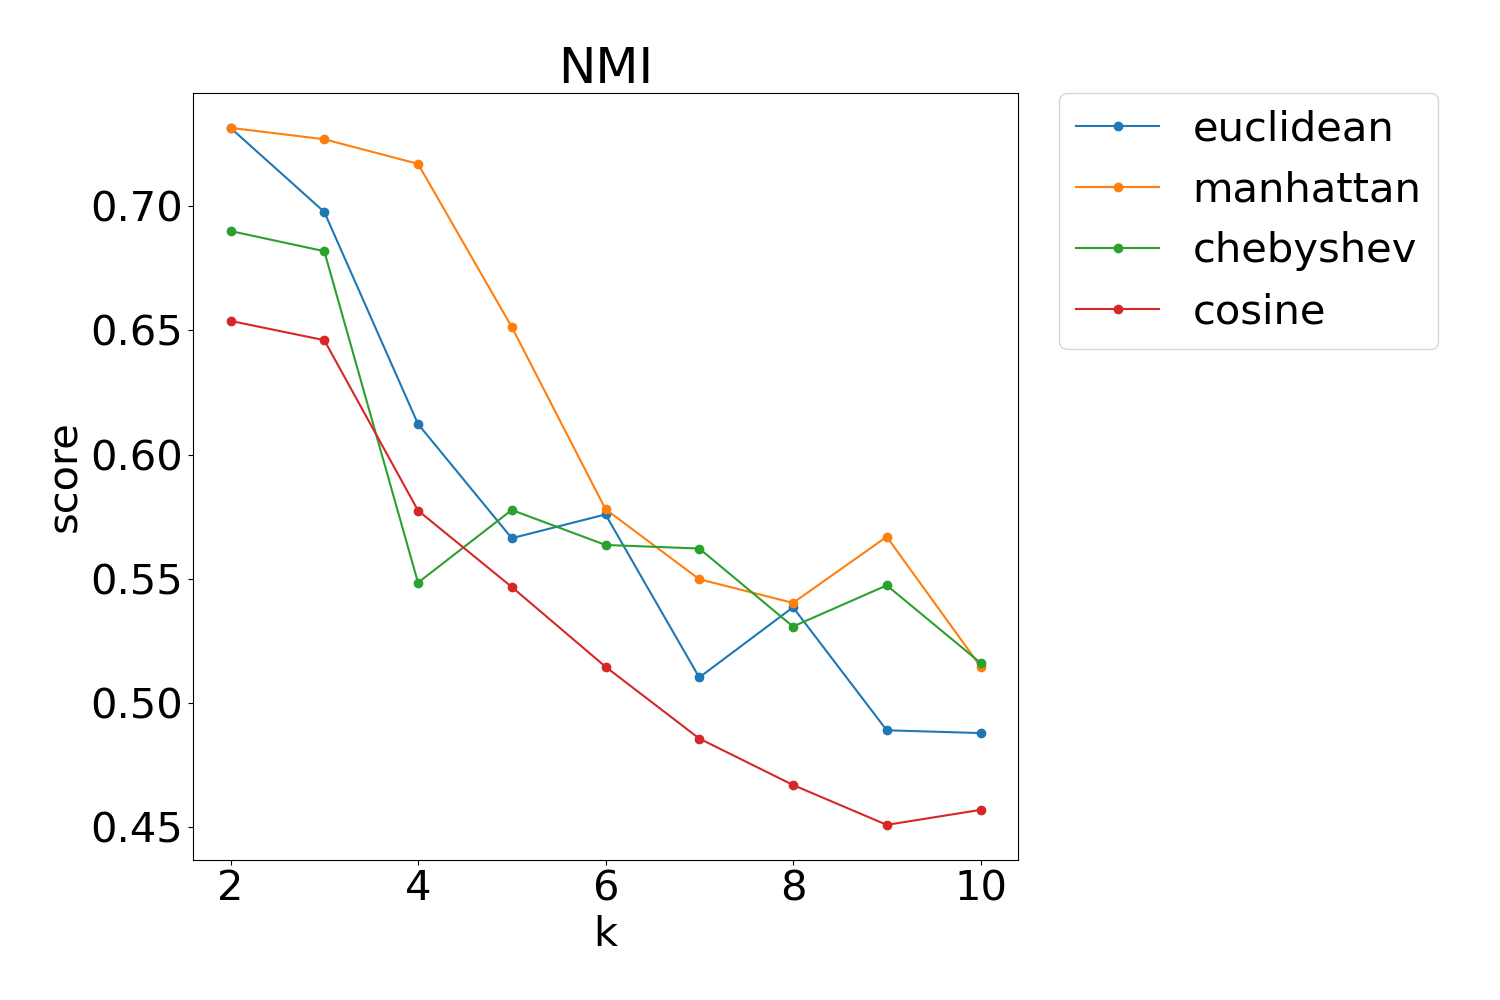
\includegraphics[width=0.45\textwidth]{../plots/iris/kmedians/NMI/k_1to10.png} }}%
	\qquad
	\subfloat[Completeness Score ]{{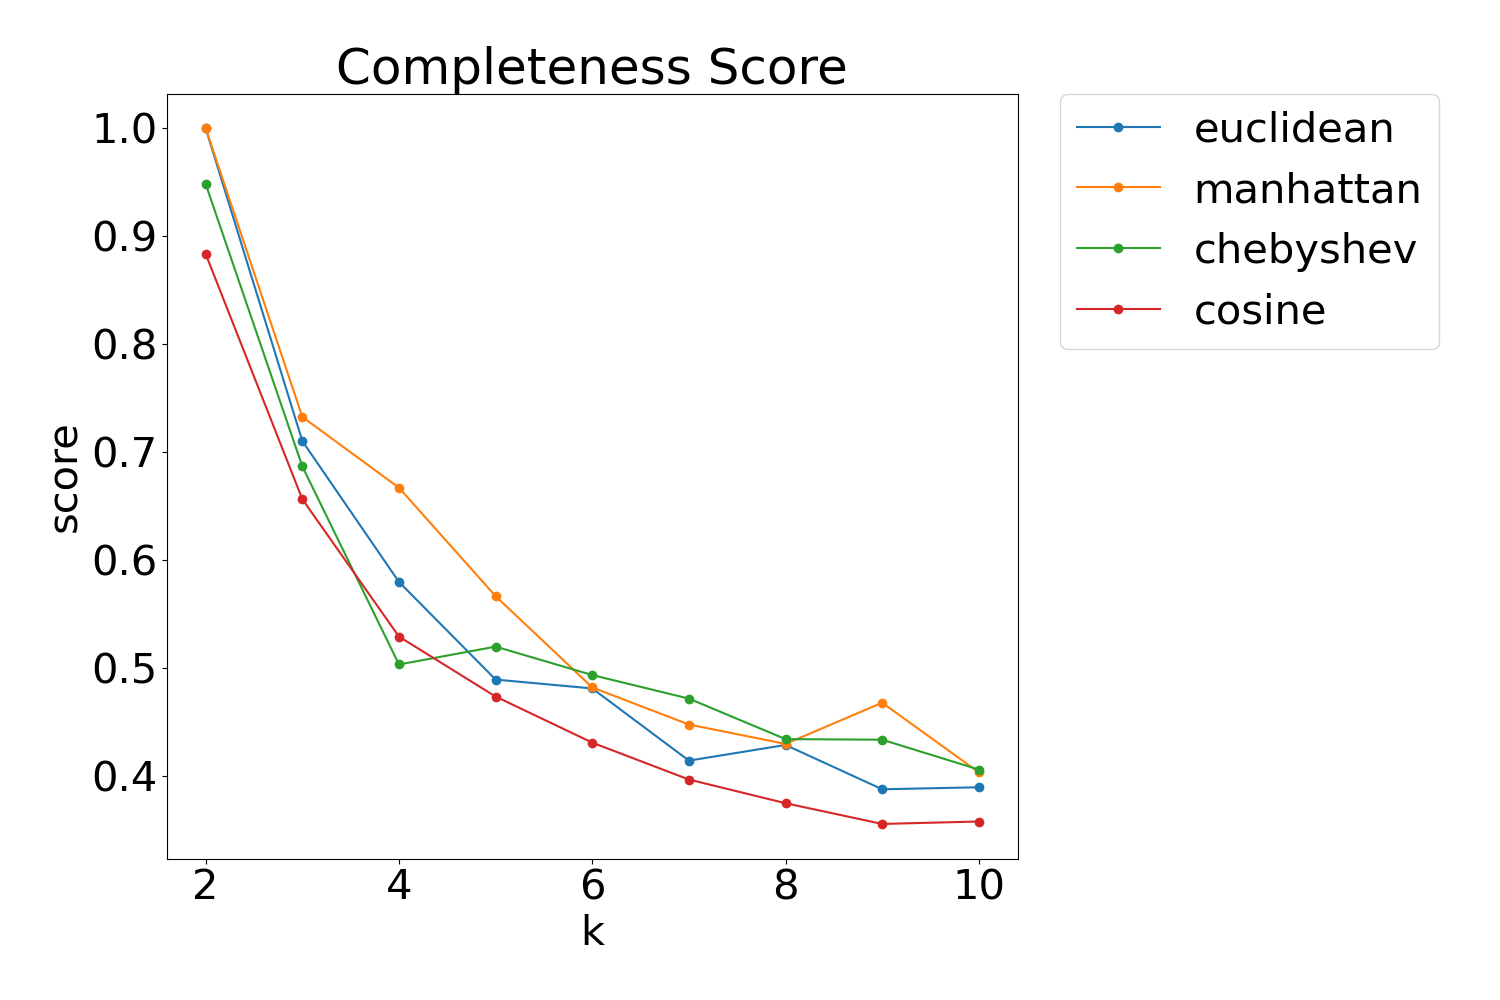
\includegraphics[width=0.45\textwidth]{../plots/iris/kmedians/Completeness Score/k_1to10.png} }}%
	\qquad
	\subfloat[Homogeneity Score ]{{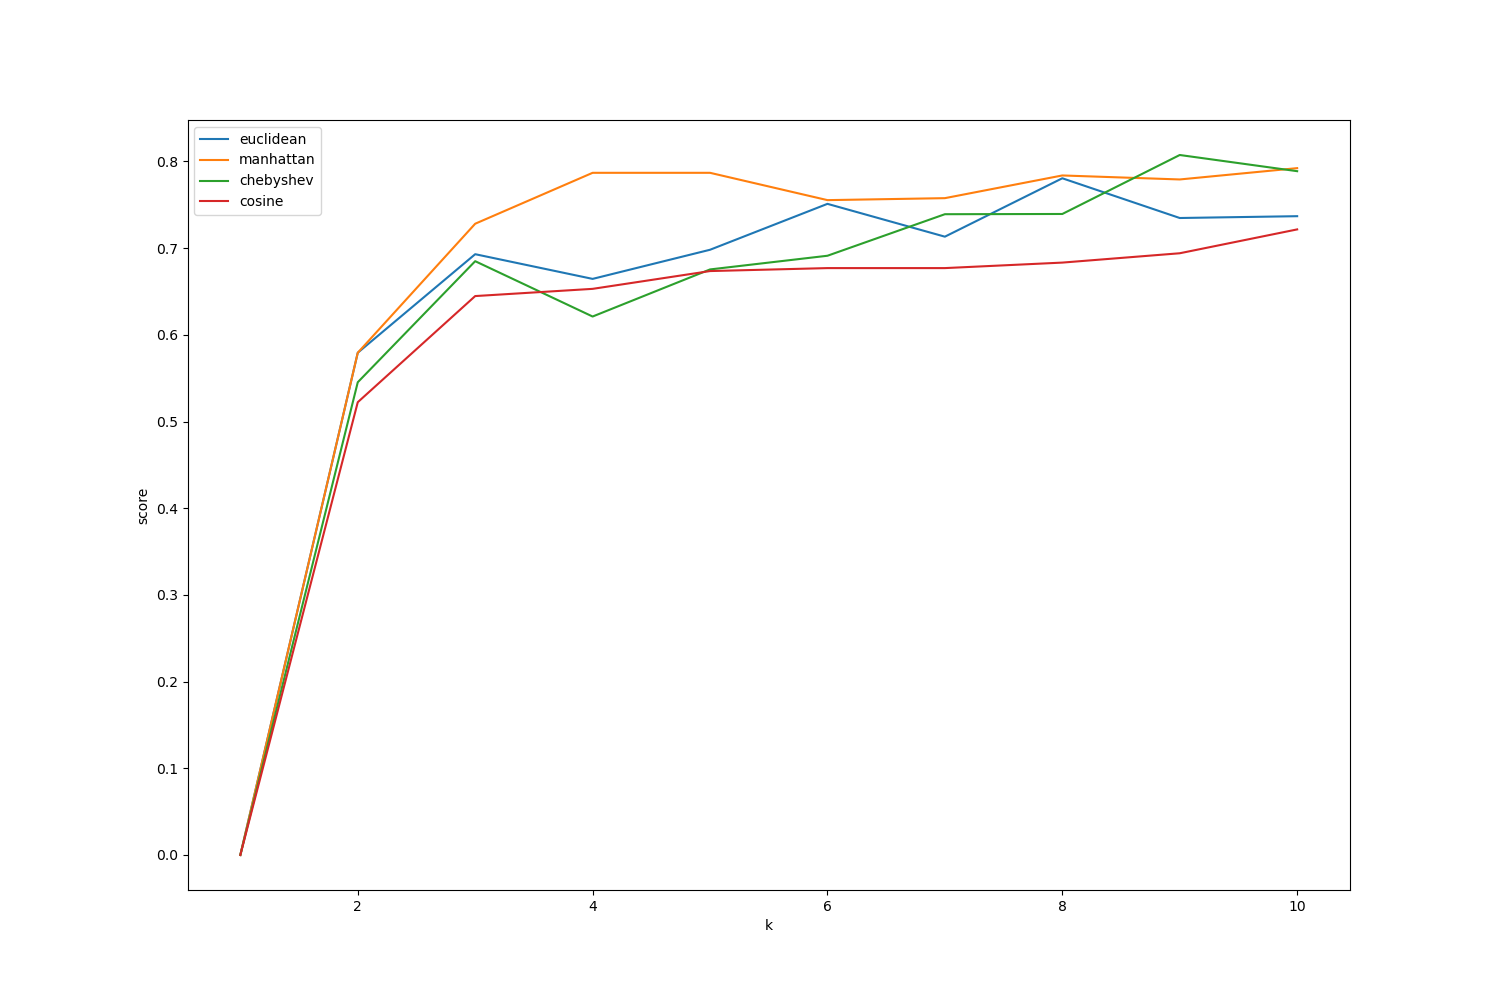
\includegraphics[width=0.45\textwidth]{../plots/iris/kmedians/Homogeneity Score/k_1to10.png} }}%
	\qquad
	\subfloat[Silhouette Score ]{{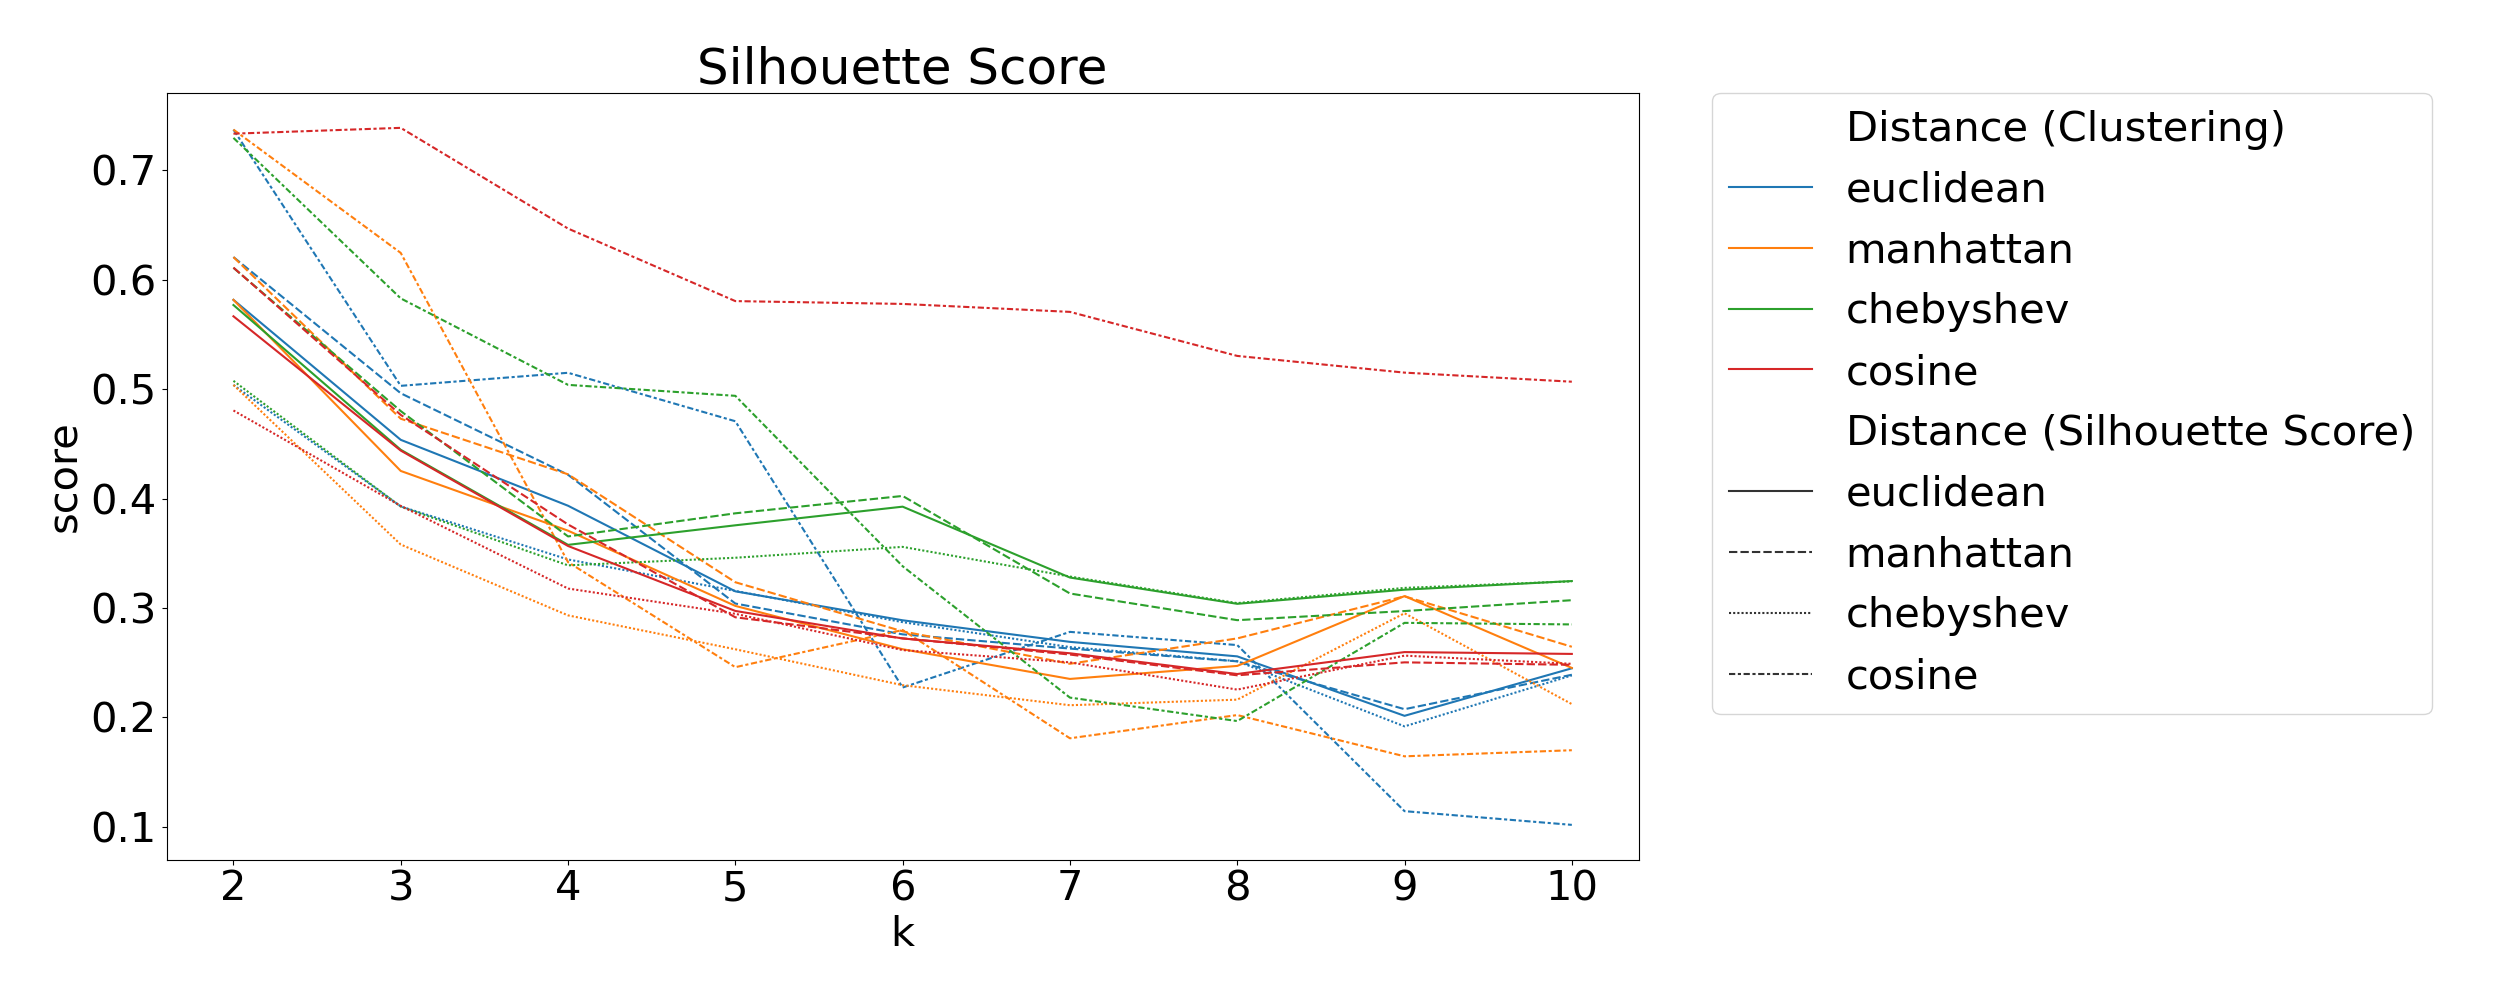
\includegraphics[width=1\textwidth]{../plots/iris/kmedians/Silhouette Score/k_1to10.png} }}%
	
	\caption{Comparison of clustering scores for kmedians-clustering on Iris dataset}%
\end{figure}

\begin{figure}[H]
	\centering
	\subfloat[ARI ]{{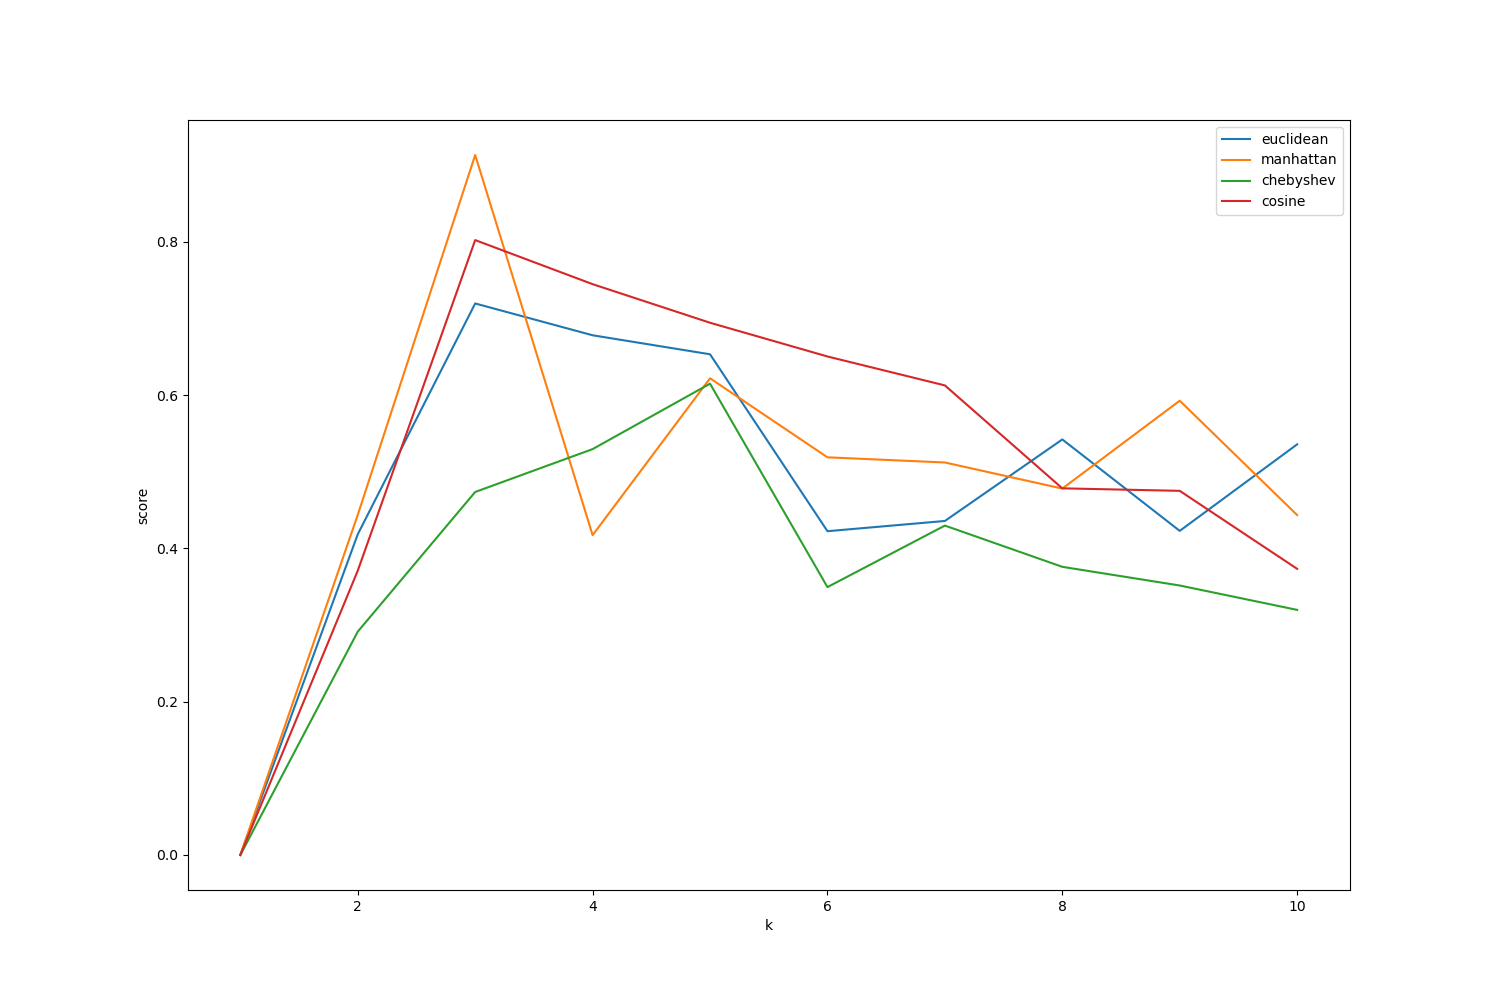
\includegraphics[width=0.45\textwidth]{../plots/wine/kmedians/ARI/k_1to10.png} }}%
	\qquad
	\subfloat[NMI ]{{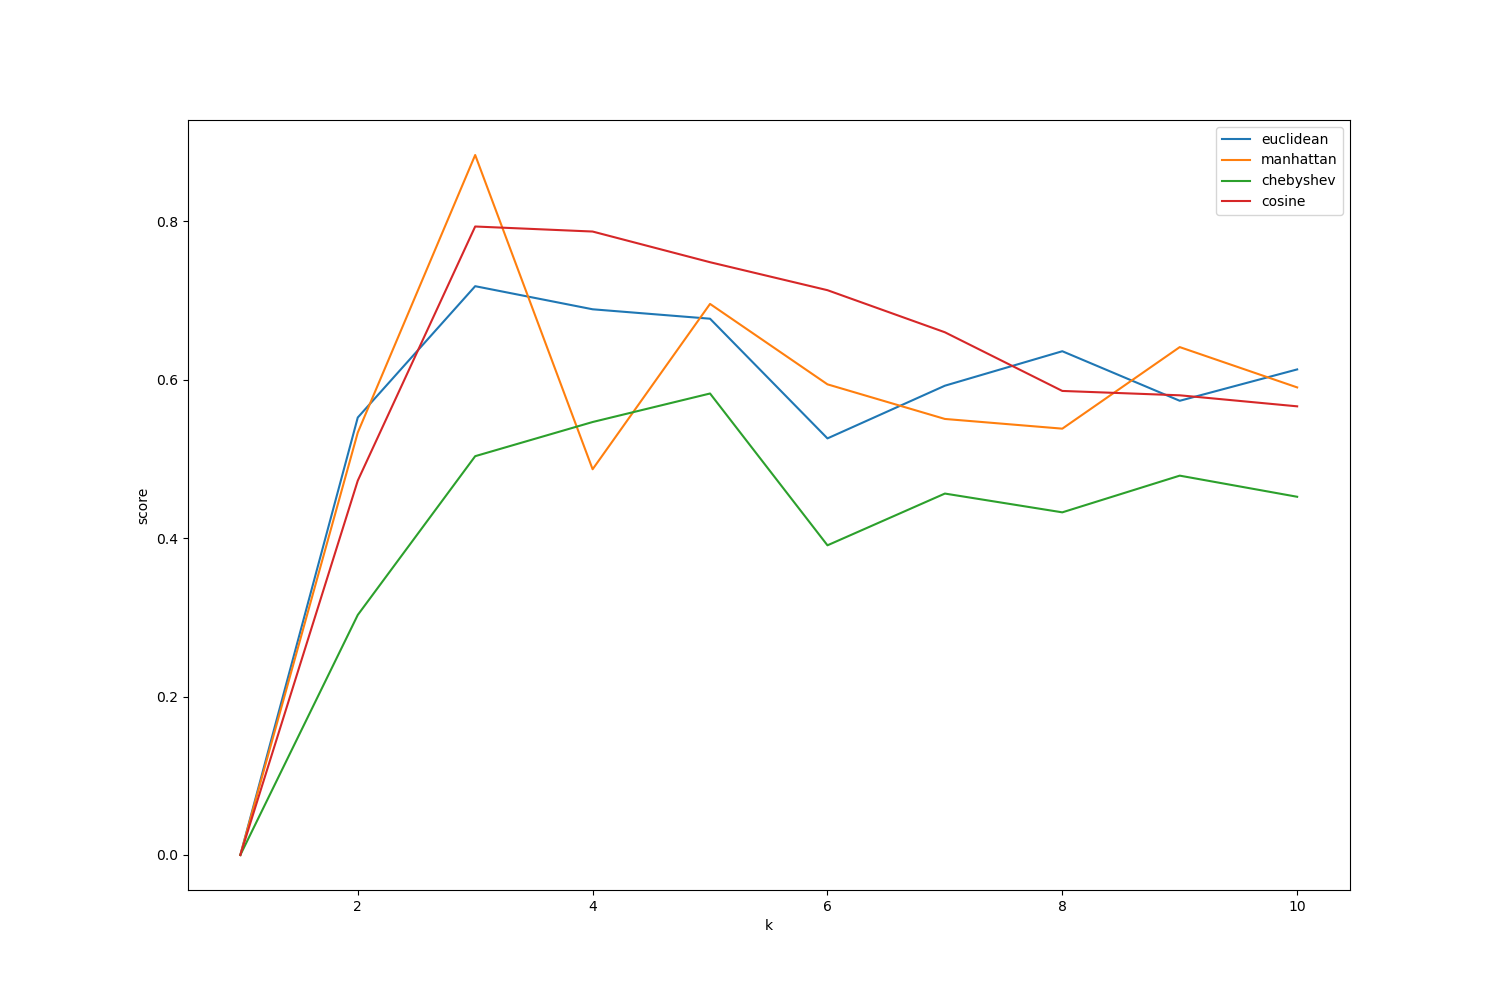
\includegraphics[width=0.45\textwidth]{../plots/wine/kmedians/NMI/k_1to10.png} }}%
	\qquad
	\subfloat[Completeness Score ]{{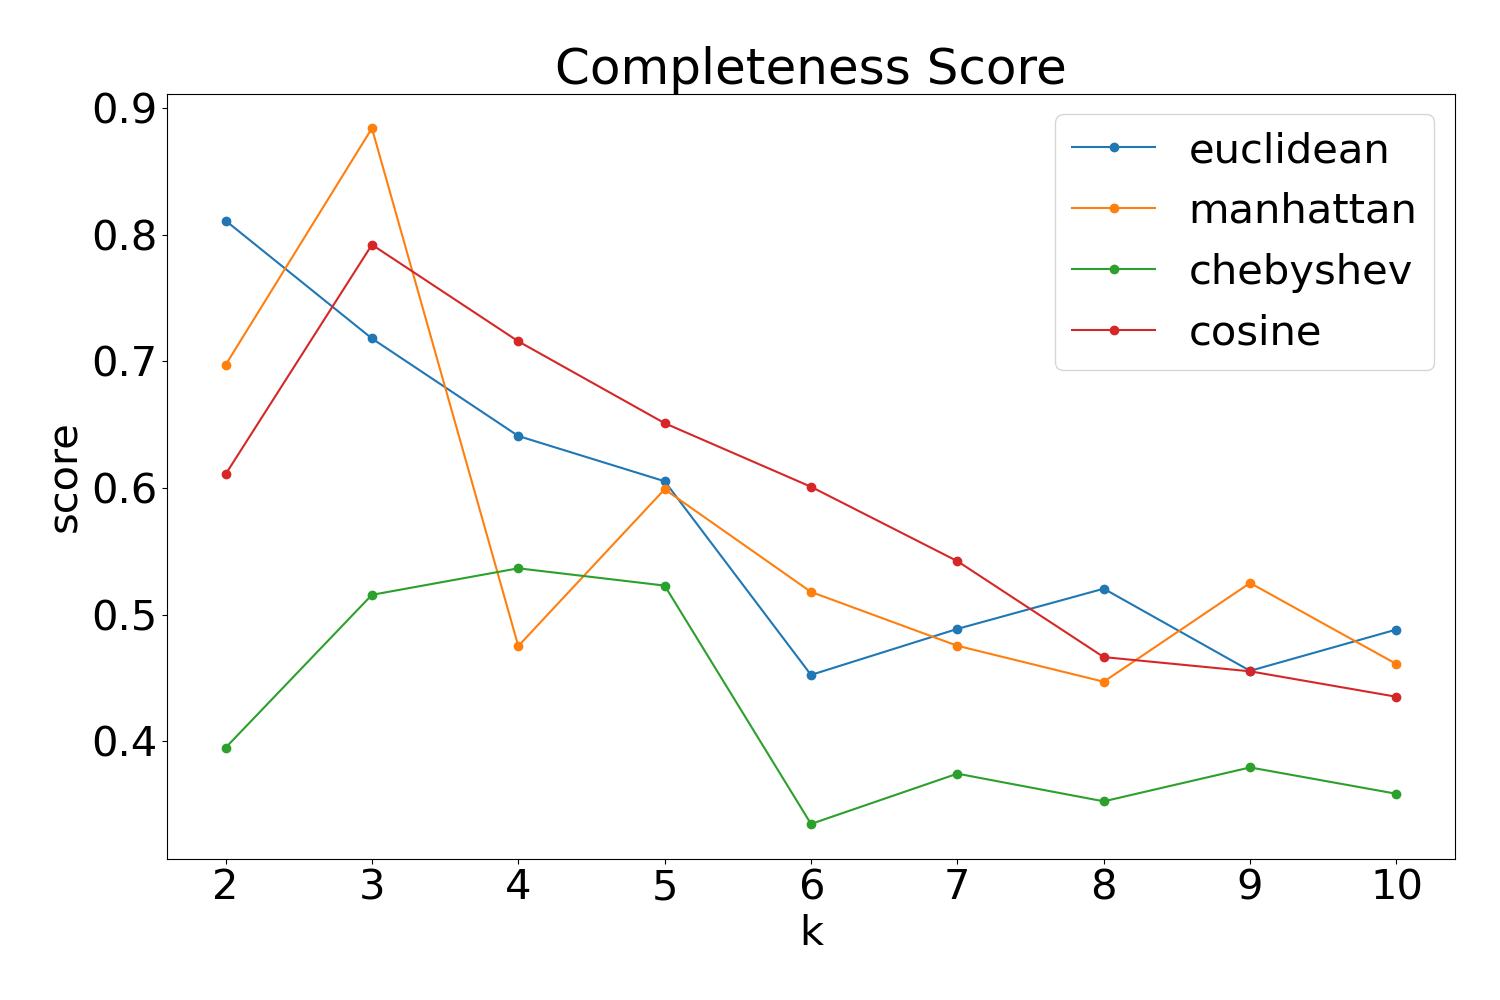
\includegraphics[width=0.45\textwidth]{../plots/wine/kmedians/Completeness Score/k_1to10.png} }}%
	\qquad
	\subfloat[Homogeneity Score ]{{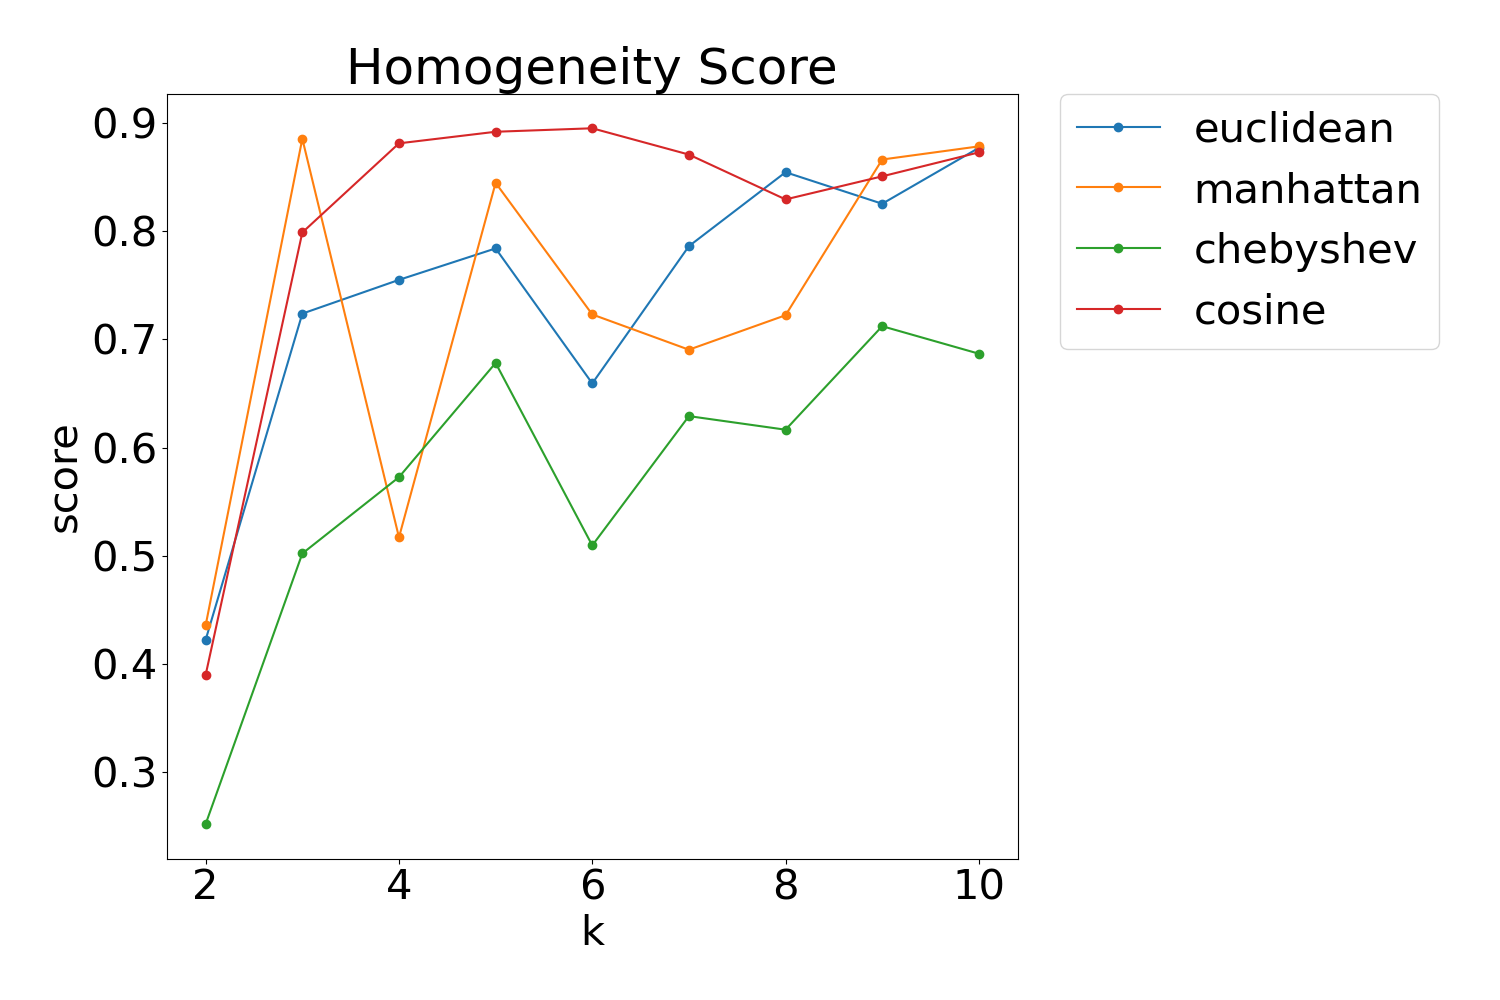
\includegraphics[width=0.45\textwidth]{../plots/wine/kmedians/Homogeneity Score/k_1to10.png} }}%
	\qquad
	\subfloat[Silhouette Score ]{{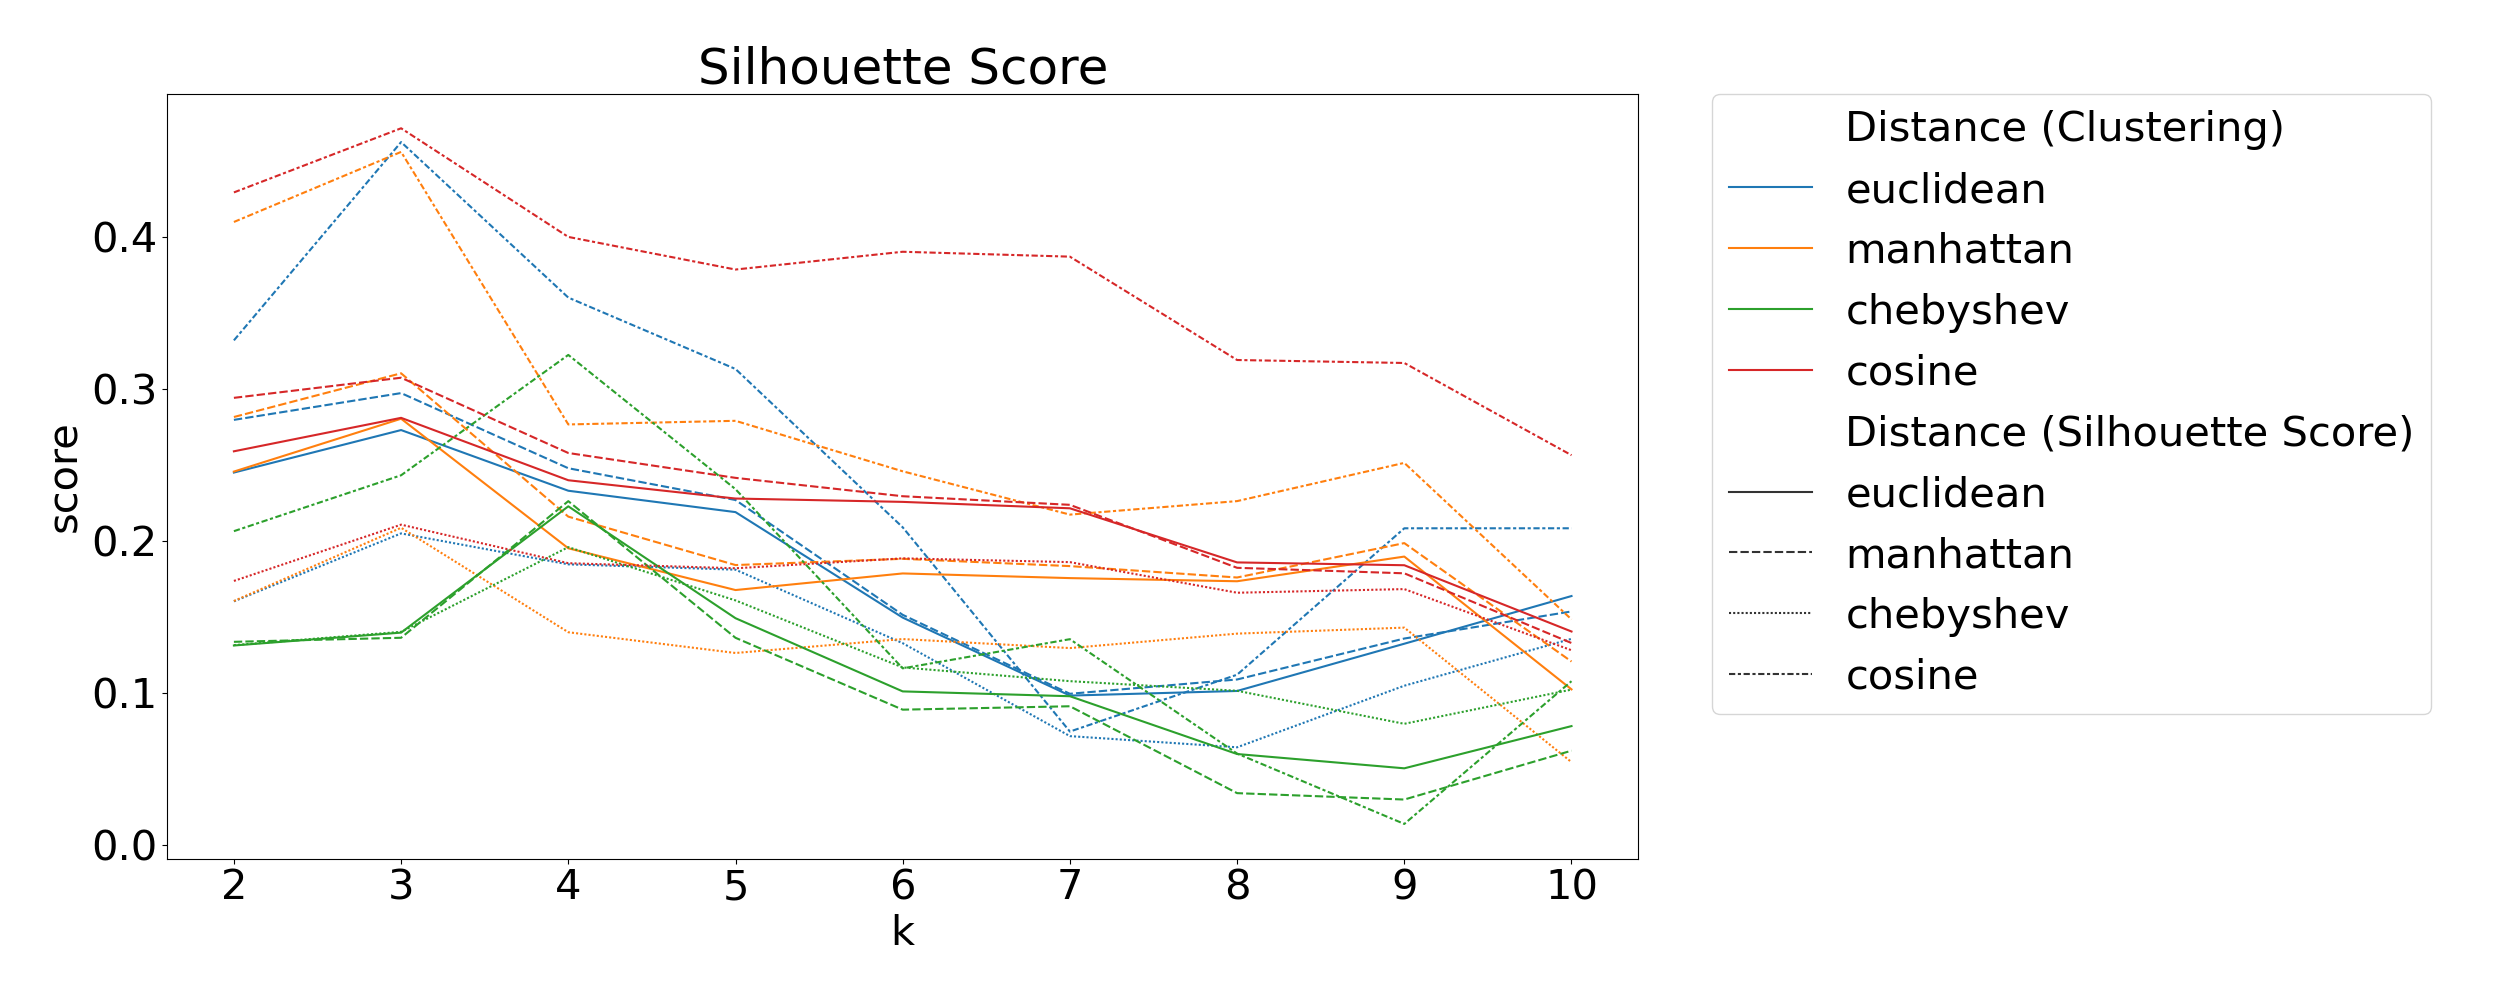
\includegraphics[width=1\textwidth]{../plots/wine/kmedians/Silhouette Score/k_1to10.png} }}%
	
	\caption{Comparison of clustering scores for kmedians-clustering on Wine dataset}%
\end{figure}

\begin{figure}[H]
	\centering
	\subfloat[Silhouette Score ]{{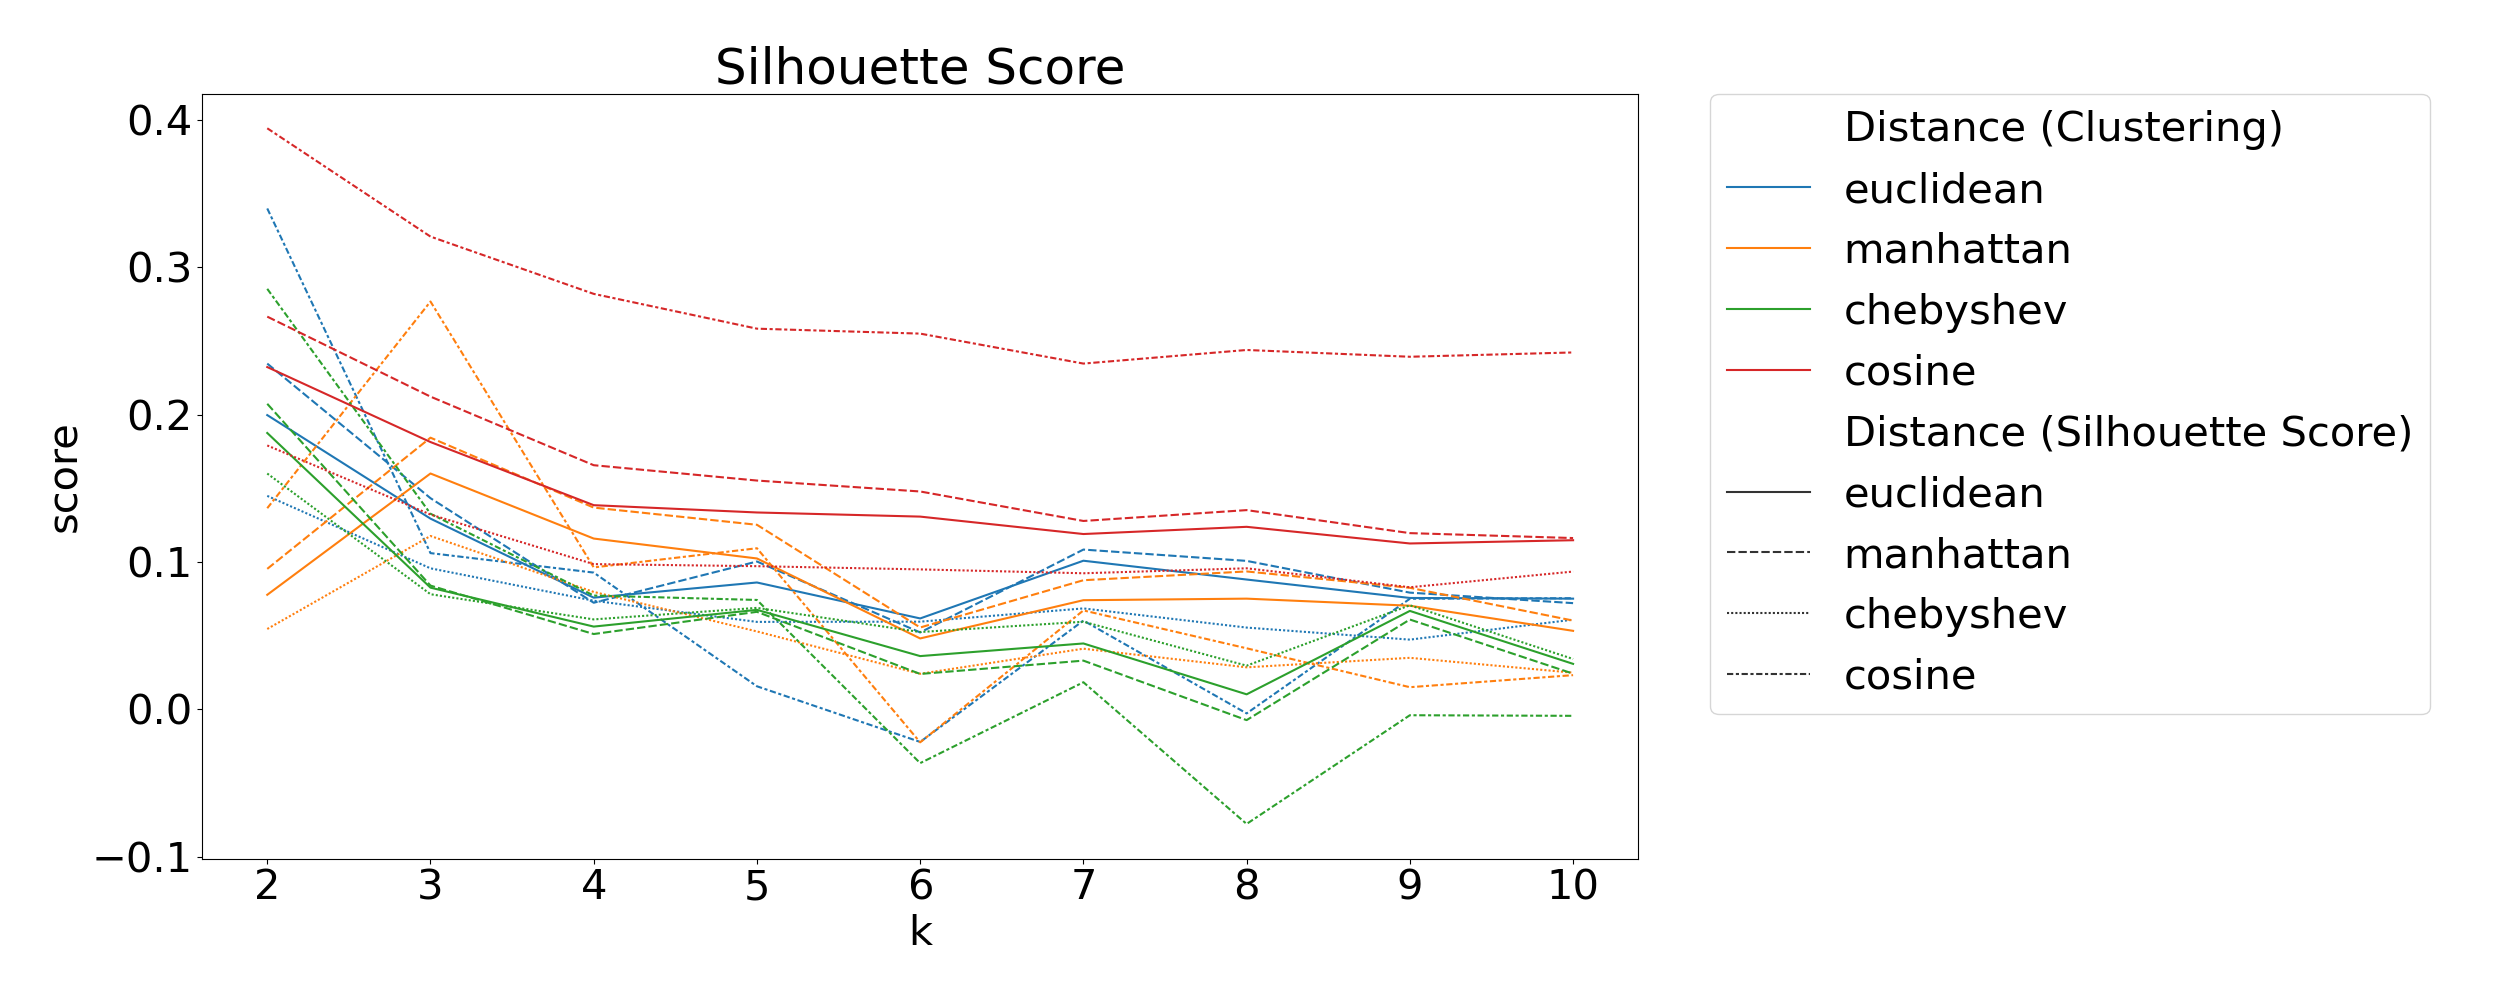
\includegraphics[width=1\textwidth]{../plots/diabetes/kmedians/Silhouette Score/k_1to10.png} }}%
	
	\caption{Comparison of clustering scores for kmedians-clustering on Diabetes dataset}%
\end{figure}

\begin{figure}[H]
	\centering
	\subfloat[ARI ]{{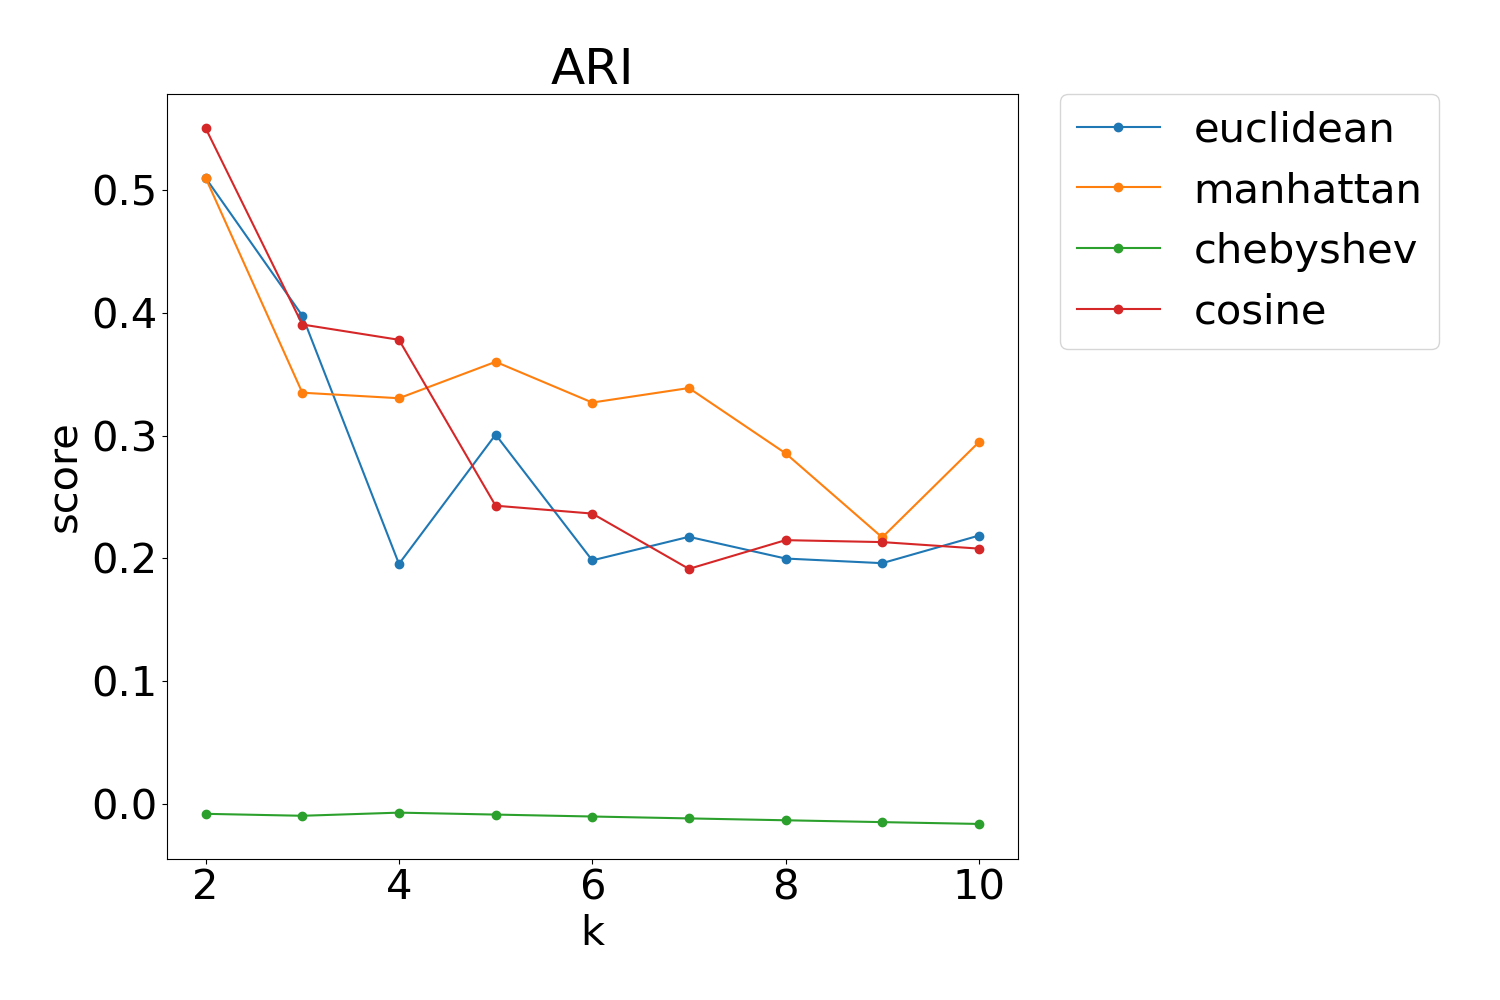
\includegraphics[width=0.45\textwidth]{../plots/housevotes/kmedians/ARI/k_1to10.png} }}%
	\qquad
	\subfloat[NMI ]{{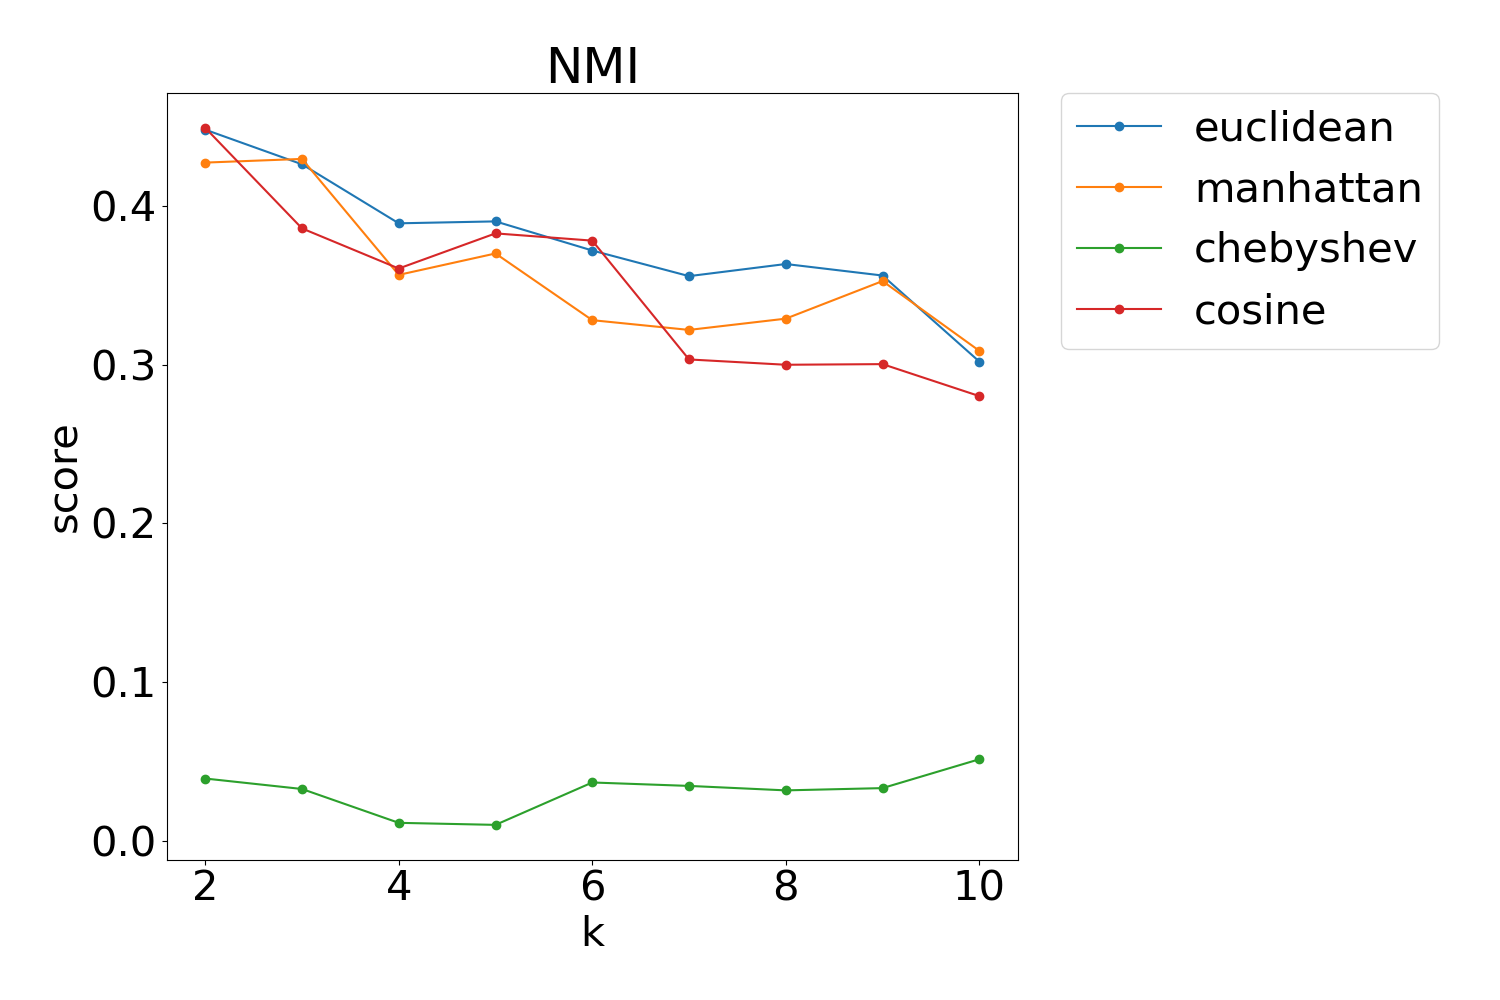
\includegraphics[width=0.45\textwidth]{../plots/housevotes/kmedians/NMI/k_1to10.png} }}%
	\qquad
	\subfloat[Completeness Score ]{{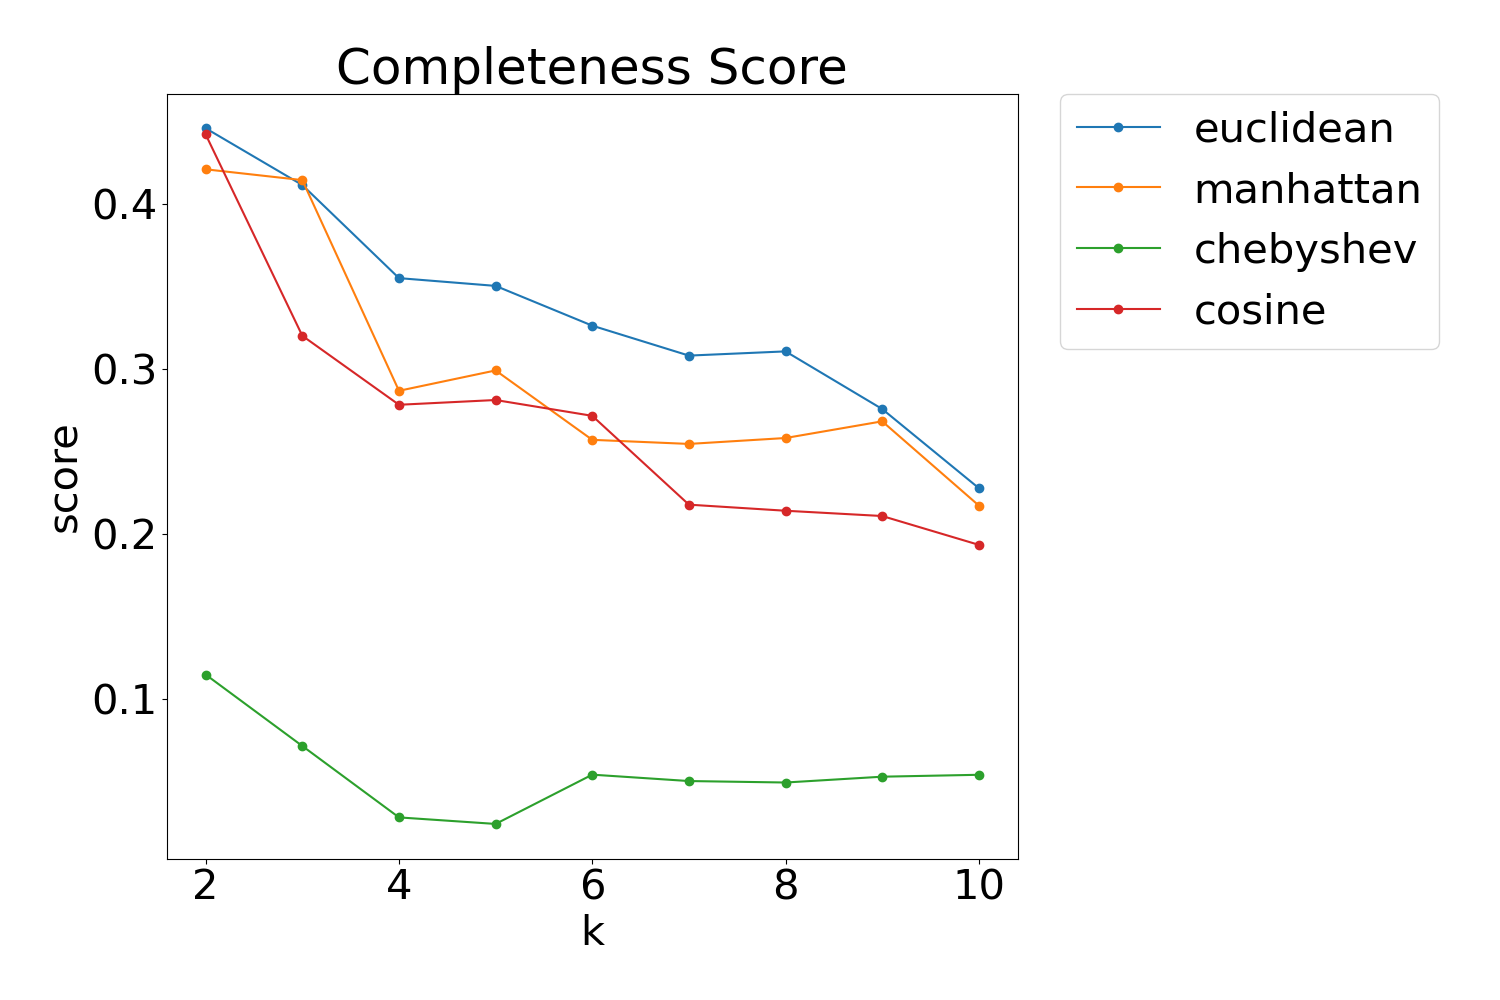
\includegraphics[width=0.45\textwidth]{../plots/housevotes/kmedians/Completeness Score/k_1to10.png} }}%
	\qquad
	\subfloat[Homogeneity Score ]{{\includegraphics[width=0.45\textwidth]{../plots/housevotes/kmedians/Homogeneity Score/k_1to10.png} }}%
	\qquad
	\subfloat[Silhouette Score ]{{\includegraphics[width=1\textwidth]{../plots/housevotes/kmedians/Silhouette Score/k_1to10.png} }}%
	
	\caption{Comparison of clustering scores for kmedians-clustering on Housevotes dataset}%
\end{figure}

\begin{figure}[H]
	\centering
	\subfloat[ARI ]{{\includegraphics[width=0.45\textwidth]{../plots/iris/kmedoids/ARI/k_1to10.png} }}%
	\qquad
	\subfloat[NMI ]{{\includegraphics[width=0.45\textwidth]{../plots/iris/kmedoids/NMI/k_1to10.png} }}%
	\qquad
	\subfloat[Completeness Score ]{{\includegraphics[width=0.45\textwidth]{../plots/iris/kmedoids/Completeness Score/k_1to10.png} }}%
	\qquad
	\subfloat[Homogeneity Score ]{{\includegraphics[width=0.45\textwidth]{../plots/iris/kmedoids/Homogeneity Score/k_1to10.png} }}%
	\qquad
	\subfloat[Silhouette Score ]{{\includegraphics[width=1\textwidth]{../plots/iris/kmedoids/Silhouette Score/k_1to10.png} }}%
	
	\caption{Comparison of clustering scores for kmedoids-clustering on Iris dataset}%
\end{figure}

\begin{figure}[H]
	\centering
	\subfloat[ARI ]{{\includegraphics[width=0.45\textwidth]{../plots/wine/kmedoids/ARI/k_1to10.png} }}%
	\qquad
	\subfloat[NMI ]{{\includegraphics[width=0.45\textwidth]{../plots/wine/kmedoids/NMI/k_1to10.png} }}%
	\qquad
	\subfloat[Completeness Score ]{{\includegraphics[width=0.45\textwidth]{../plots/wine/kmedoids/Completeness Score/k_1to10.png} }}%
	\qquad
	\subfloat[Homogeneity Score ]{{\includegraphics[width=0.45\textwidth]{../plots/wine/kmedoids/Homogeneity Score/k_1to10.png} }}%
	\qquad
	\subfloat[Silhouette Score ]{{\includegraphics[width=1\textwidth]{../plots/wine/kmedoids/Silhouette Score/k_1to10.png} }}%
	
	\caption{Comparison of clustering scores for kmedoids-clustering on Wine dataset}%
\end{figure}

\begin{figure}[H]
	\centering
	\subfloat[Silhouette Score ]{{\includegraphics[width=1\textwidth]{../plots/diabetes/kmedoids/Silhouette Score/k_1to10.png} }}%
	
	\caption{Comparison of clustering scores for kmedoids-clustering on Diabetes dataset}%
\end{figure}

\begin{figure}[H]
	\centering
	\subfloat[ARI ]{{\includegraphics[width=0.45\textwidth]{../plots/housevotes/kmedoids/ARI/k_1to10.png} }}%
	\qquad
	\subfloat[NMI ]{{\includegraphics[width=0.45\textwidth]{../plots/housevotes/kmedoids/NMI/k_1to10.png} }}%
	\qquad
	\subfloat[Completeness Score ]{{\includegraphics[width=0.45\textwidth]{../plots/housevotes/kmedoids/Completeness Score/k_1to10.png} }}%
	\qquad
	\subfloat[Homogeneity Score ]{{\includegraphics[width=0.45\textwidth]{../plots/housevotes/kmedoids/Homogeneity Score/k_1to10.png} }}%
	\qquad
	\subfloat[Silhouette Score ]{{\includegraphics[width=1\textwidth]{../plots/housevotes/kmedoids/Silhouette Score/k_1to10.png} }}%
	
	\caption{Comparison of clustering scores for kmedoids-clustering on Housevotes dataset}%
\end{figure}

